%% bare_jrnl_compsoc.tex
%% V1.4b
%% 2015/08/26
%% by Michael Shell
%% See:
%% http://www.michaelshell.org/
%% for current contact information.
%%
%% This is a skeleton file demonstrating the use of IEEEtran.cls
%% (requires IEEEtran.cls version 1.8b or later) with an IEEE
%% Computer Society journal paper.
%%
%% Support sites:
%% http://www.michaelshell.org/tex/ieeetran/
%% http://www.ctan.org/pkg/ieeetran
%% and
%% http://www.ieee.org/

%%*************************************************************************
%% Legal Notice:
%% This code is offered as-is without any warranty either expressed or
%% implied; without even the implied warranty of MERCHANTABILITY or
%% FITNESS FOR A PARTICULAR PURPOSE! 
%% User assumes all risk.
%% In no event shall the IEEE or any contributor to this code be liable for
%% any damages or losses, including, but not limited to, incidental,
%% consequential, or any other damages, resulting from the use or misuse
%% of any information contained here.
%%
%% All comments are the opinions of their respective authors and are not
%% necessarily endorsed by the IEEE.
%%
%% This work is distributed under the LaTeX Project Public License (LPPL)
%% ( http://www.latex-project.org/ ) version 1.3, and may be freely used,
%% distributed and modified. A copy of the LPPL, version 1.3, is included
%% in the base LaTeX documentation of all distributions of LaTeX released
%% 2003/12/01 or later.
%% Retain all contribution notices and credits.
%% ** Modified files should be clearly indicated as such, including  **
%% ** renaming them and changing author support contact information. **
%%*************************************************************************


% *** Authors should verify (and, if needed, correct) their LaTeX system  ***
% *** with the testflow diagnostic prior to trusting their LaTeX platform ***
% *** with production work. The IEEE's font choices and paper sizes can   ***
% *** trigger bugs that do not appear when using other class files.       ***                          ***
% The testflow support page is at:
% http://www.michaelshell.org/tex/testflow/


\documentclass[10pt,journal,compsoc]{IEEEtran}
%
% If IEEEtran.cls has not been installed into the LaTeX system files,
% manually specify the path to it like:
% \documentclass[10pt,journal,compsoc]{../sty/IEEEtran}





% Some very useful LaTeX packages include:
% (uncomment the ones you want to load)


% *** MISC UTILITY PACKAGES ***
%
%\usepackage{ifpdf}
% Heiko Oberdiek's ifpdf.sty is very useful if you need conditional
% compilation based on whether the output is pdf or dvi.
% usage:
% \ifpdf
%   % pdf code
% \else
%   % dvi code
% \fi
% The latest version of ifpdf.sty can be obtained from:
% http://www.ctan.org/pkg/ifpdf
% Also, note that IEEEtran.cls V1.7 and later provides a builtin
% \ifCLASSINFOpdf conditional that works the same way.
% When switching from latex to pdflatex and vice-versa, the compiler may
% have to be run twice to clear warning/error messages.






% *** CITATION PACKAGES ***
%
\ifCLASSOPTIONcompsoc
  % IEEE Computer Society needs nocompress option
  % requires cite.sty v4.0 or later (November 2003)
  \usepackage[nocompress]{cite}
\else
  % normal IEEE
  \usepackage{cite}
\fi

% cite.sty was written by Donald Arseneau
% V1.6 and later of IEEEtran pre-defines the format of the cite.sty package
% \cite{} output to follow that of the IEEE. Loading the cite package will
% result in citation numbers being automatically sorted and properly
% "compressed/ranged". e.g., [1], [9], [2], [7], [5], [6] without using
% cite.sty will become [1], [2], [5]--[7], [9] using cite.sty. cite.sty's
% \cite will automatically add leading space, if needed. Use cite.sty's
% noadjust option (cite.sty V3.8 and later) if you want to turn this off
% such as if a citation ever needs to be enclosed in parenpaper.
% cite.sty is already installed on most LaTeX systems. Be sure and use
% version 5.0 (2009-03-20) and later if using hyperref.sty.
% The latest version can be obtained at:
% http://www.ctan.org/pkg/cite
% The documentation is contained in the cite.sty file itself.
%
% Note that some packages require special options to format as the Computer
% Society requires. In particular, Computer Society  papers do not use
% compressed citation ranges as is done in typical IEEE papers
% (e.g., [1]-[4]). Instead, they list every citation separately in order
% (e.g., [1], [2], [3], [4]). To get the latter we need to load the cite
% package with the nocompress option which is supported by cite.sty v4.0
% and later. Note also the use of a CLASSOPTION conditional provided by
% IEEEtran.cls V1.7 and later.






% *** GRAPHICS RELATED PACKAGES ***
%
\ifCLASSINFOpdf
   \usepackage[pdftex]{graphicx}
  % declare the path(s) where your graphic files are
  \graphicspath{{figures/}}
    % and their extensions so you won't have to specify these with
  % every instance of \includegraphics
   \DeclareGraphicsExtensions{.pdf,.jpeg,.png}
\else
  % or other class option (dvipsone, dvipdf, if not using dvips). graphicx
  % will default to the driver specified in the system graphics.cfg if no
  % driver is specified.
  % \usepackage[dvips]{graphicx}
  % declare the path(s) where your graphic files are
  % \graphicspath{{../eps/}}
  % and their extensions so you won't have to specify these with
  % every instance of \includegraphics
  % \DeclareGraphicsExtensions{.eps}
\fi
% graphicx was written by David Carlisle and Sebastian Rahtz. It is
% required if you want graphics, photos, etc. graphicx.sty is already
% installed on most LaTeX systems. The latest version and documentation
% can be obtained at: 
% http://www.ctan.org/pkg/graphicx
% Another good source of documentation is "Using Imported Graphics in
% LaTeX2e" by Keith Reckdahl which can be found at:
% http://www.ctan.org/pkg/epslatex
%
% latex, and pdflatex in dvi mode, support graphics in encapsulated
% postscript (.eps) format. pdflatex in pdf mode supports graphics
% in .pdf, .jpeg, .png and .mps (metapost) formats. Users should ensure
% that all non-photo figures use a vector format (.eps, .pdf, .mps) and
% not a bitmapped formats (.jpeg, .png). The IEEE frowns on bitmapped formats
% which can result in "jaggedy"/blurry rendering of lines and letters as
% well as large increases in file sizes.
%
% You can find documentation about the pdfTeX application at:
% http://www.tug.org/applications/pdftex


\usepackage{float}
\usepackage{colortbl}
\usepackage[table*]{xcolor}
\xdefinecolor{gray95}{gray}{0.65}
\xdefinecolor{gray25}{gray}{0.8}
\xdefinecolor{blizzardblue}{rgb}{0.67,0.67,0.67}
%\usepackage{booktabs,siunitx}


% *** MATH PACKAGES ***
%
\usepackage{amsmath}
\usepackage{amsfonts}
% A popular package from the American Mathematical Society that provides
% many useful and powerful commands for dealing with mathematics.
%
% Note that the amsmath package sets \interdisplaylinepenalty to 10000
% thus preventing page breaks from occurring within multiline equations. Use:
%\interdisplaylinepenalty=2500
% after loading amsmath to restore such page breaks as IEEEtran.cls normally
% does. amsmath.sty is already installed on most LaTeX systems. The latest
% version and documentation can be obtained at:
% http://www.ctan.org/pkg/amsmath





% *** SPECIALIZED LIST PACKAGES ***
%

\usepackage{algorithmic}
%\algnewcommand\algorithmicforeach{\textbf{for each}}
%\algdef{S}[FOR]{ForEach}[1]{\algorithmicforeach\ #1\ \algorithmicdo}

% algorithmic.sty was written by Peter Williams and Rogerio Brito.
% This package provides an algorithmic environment fo describing algorithms.
% You can use the algorithmic environment in-text or within a figure
% environment to provide for a floating algorithm. Do NOT use the algorithm
% floating environment provided by algorithm.sty (by the same authors) or
% algorithm2e.sty (by Christophe Fiorio) as the IEEE does not use dedicated
% algorithm float types and packages that provide these will not provide
% correct IEEE style captions. The latest version and documentation of
% algorithmic.sty can be obtained at:
% http://www.ctan.org/pkg/algorithms
% Also of interest may be the (relatively newer and more customizable)
% algorithmicx.sty package by Szasz Janos:
% http://www.ctan.org/pkg/algorithmicx




% *** ALIGNMENT PACKAGES ***
%
\usepackage{array}
% Frank Mittelbach's and David Carlisle's array.sty patches and improves
% the standard LaTeX2e array and tabular environments to provide better
% appearance and additional user controls. As the default LaTeX2e table
% generation code is lacking to the point of almost being broken with
% respect to the quality of the end results, all users are strongly
% advised to use an enhanced (at the very least that provided by array.sty)
% set of table tools. array.sty is already installed on most systems. The
% latest version and documentation can be obtained at:
% http://www.ctan.org/pkg/array


% IEEEtran contains the IEEEeqnarray family of commands that can be used to
% generate multiline equations as well as matrices, tables, etc., of high
% quality.




% *** SUBFIGURE PACKAGES ***
%\ifCLASSOPTIONcompsoc
  \usepackage[caption=false,font=footnotesize,labelfont=sf,textfont=sf]{subfig}
%\else
 % \usepackage[caption=false,font=footnotesize]{subfig}
%\fi
% subfig.sty, written by Steven Douglas Cochran, is the modern replacement
% for subfigure.sty, the latter of which is no longer maintained and is
% incompatible with some LaTeX packages including fixltx2e. However,
% subfig.sty requires and automatically loads Axel Sommerfeldt's caption.sty
% which will override IEEEtran.cls' handling of captions and this will result
% in non-IEEE style figure/table captions. To prevent this problem, be sure
% and invoke subfig.sty's "caption=false" package option (available since
% subfig.sty version 1.3, 2005/06/28) as this is will preserve IEEEtran.cls
% handling of captions.
% Note that the Computer Society format requires a sans serif font rather
% than the serif font used in traditional IEEE formatting and thus the need
% to invoke different subfig.sty package options depending on whether
% compsoc mode has been enabled.
%
% The latest version and documentation of subfig.sty can be obtained at:
% http://www.ctan.org/pkg/subfig




% *** FLOAT PACKAGES ***
%
%\usepackage{fixltx2e}
% fixltx2e, the successor to the earlier fix2col.sty, was written by
% Frank Mittelbach and David Carlisle. This package corrects a few problems
% in the LaTeX2e kernel, the most notable of which is that in current
% LaTeX2e releases, the ordering of single and double column floats is not
% guaranteed to be preserved. Thus, an unpatched LaTeX2e can allow a
% single column figure to be placed prior to an earlier double column
% figure.
% Be aware that LaTeX2e kernels dated 2015 and later have fixltx2e.sty's
% corrections already built into the system in which case a warning will
% be issued if an attempt is made to load fixltx2e.sty as it is no longer
% needed.
% The latest version and documentation can be found at:
% http://www.ctan.org/pkg/fixltx2e


%\usepackage{stfloats}
% stfloats.sty was written by Sigitas Tolusis. This package gives LaTeX2e
% the ability to do double column floats at the bottom of the page as well
% as the top. (e.g., "\begin{figure*}[!b]" is not normally possible in
% LaTeX2e). It also provides a command:
%\fnbelowfloat
% to enable the placement of footnotes below bottom floats (the standard
% LaTeX2e kernel puts them above bottom floats). This is an invasive package
% which rewrites many portions of the LaTeX2e float routines. It may not work
% with other packages that modify the LaTeX2e float routines. The latest
% version and documentation can be obtained at:
% http://www.ctan.org/pkg/stfloats
% Do not use the stfloats baselinefloat ability as the IEEE does not allow
% \baselineskip to stretch. Authors submitting work to the IEEE should note
% that the IEEE rarely uses double column equations and that authors should try
% to avoid such use. Do not be tempted to use the cuted.sty or midfloat.sty
% packages (also by Sigitas Tolusis) as the IEEE does not format its papers in
% such ways.
% Do not attempt to use stfloats with fixltx2e as they are incompatible.
% Instead, use Morten Hogholm'a dblfloatfix which combines the features
% of both fixltx2e and stfloats:
%
% \usepackage{dblfloatfix}
% The laest version can be found at:
% http://www.ctan.org/pkg/dblfloatfix

\usepackage{caption}% http://ctan.org/pkg/caption
\captionsetup[table]{format=plain,labelformat=simple,labelsep=period}%

%\ifCLASSOPTIONcaptionsoff
 % \usepackage[nomarkers]{endfloat}
 %\let\MYoriglatexcaption\caption
 %\renewcommand{\caption}[2][\relax]{\MYoriglatexcaption[#2]{#2}}
%\fi
% endfloat.sty was written by James Darrell McCauley, Jeff Goldberg and 
% Axel Sommerfeldt. This package may be useful when used in conjunction with 
% IEEEtran.cls'  captionsoff option. Some IEEE journals/societies require that
% submissions have lists of figures/tables at the end of the paper and that
% figures/tables without any captions are placed on a page by themselves at
% the end of the document. If needed, the draftcls IEEEtran class option or
% \CLASSINPUTbaselinestretch interface can be used to increase the line
% spacing as well. Be sure and use the nomarkers option of endfloat to
% prevent endfloat from "marking" where the figures would have been placed
% in the text. The two hack lines of code above are a slight modification of
% that suggested by in the endfloat docs (section 8.4.1) to ensure that
% the full captions always appear in the list of figures/tables - even if
% the user used the short optional argument of \caption[]{}.
% IEEE papers do not typically make use of \caption[]'s optional argument,
% so this should not be an issue. A similar trick can be used to disable
% captions of packages such as subfig.sty that lack options to turn off
% the subcaptions:
% For subfig.sty:
% \let\MYorigsubfloat\subfloat
% \renewcommand{\subfloat}[2][\relax]{\MYorigsubfloat[]{#2}}
% However, the above trick will not work if both optional arguments of
% the \subfloat command are used. Furthermore, there needs to be a
% description of each subfigure *somewhere* and endfloat does not add
% subfigure captions to its list of figures. Thus, the best approach is to
% avoid the use of subfigure captions (many IEEE journals avoid them anyway)
% and instead reference/explain all the subfigures within the main caption.
% The latest version of endfloat.sty and its documentation can obtained at:
% http://www.ctan.org/pkg/endfloat
%
% The IEEEtran \ifCLASSOPTIONcaptionsoff conditional can also be used
% later in the document, say, to conditionally put the References on a 
% page by themselves.




% *** PDF, URL AND HYPERLINK PACKAGES ***
%
\usepackage{url}
% url.sty was written by Donald Arseneau. It provides better support for
% handling and breaking URLs. url.sty is already installed on most LaTeX
% systems. The latest version and documentation can be obtained at:
% http://www.ctan.org/pkg/url
% Basically, \url{my_url_here}.





% *** Do not adjust lengths that control margins, column widths, etc. ***
% *** Do not use packages that alter fonts (such as pslatex).         ***
% There should be no need to do such things with IEEEtran.cls V1.6 and later.
% (Unless specifically asked to do so by the journal or conference you plan
% to submit to, of course. )
\newcommand{\Fig}[1]{Fig.~\ref{#1}}
\newcommand{\Figure}[1]{Figure~\ref{#1}}
\newcommand{\Eq}[1]{(\ref{#1})}

% correct bad hyphenation here
\hyphenation{op-tical net-works semi-conduc-tor}


\begin{document}
%
% paper title
% Titles are generally capitalized except for words such as a, an, and, as,
% at, but, by, for, in, nor, of, on, or, the, to and up, which are usually
% not capitalized unless they are the first or last word of the title.
% Linebreaks \\ can be used within to get better formatting as desired.
% Do not put math or special symbols in the title.
\title{Towards a Planning and Design of Fog Networks}
%
%
% author names and IEEE memberships
% note positions of commas and nonbreaking spaces ( ~ ) LaTeX will not break
% a structure at a ~ so this keeps an author's name from being broken across
% two lines.
% use \thanks{} to gain access to the first footnote area
% a separate \thanks must be used for each paragraph as LaTeX2e's \thanks
% was not built to handle multiple paragraphs
%
%
%\IEEEcompsocitemizethanks is a special \thanks that produces the bulleted
% lists the Computer Society journals use for "first footnote" author
% affiliations. Use \IEEEcompsocthanksitem which works much like \item
% for each affiliation group. When not in compsoc mode,
% \IEEEcompsocitemizethanks becomes like \thanks and
% \IEEEcompsocthanksitem becomes a line break with idention. This
% facilitates dual compilation, although admittedly the differences in the
% desired content of \author between the different types of papers makes a
% one-size-fits-all approach a daunting prospect. For instance, compsoc 
% journal papers have the author affiliations above the "Manuscript
% received ..."  text while in non-compsoc journals this is reversed. Sigh.

\author{Decheng~Zhang, %~\IEEEmembership{Member,~IEEE,}
        Faisal~Haider, %~\IEEEmembership{Fellow,~OSA,}
        Marc St-Hilaire %
        and~Christian~Makaya%,~\IEEEmembership{Life~Fellow,~IEEE}% <-this % stops a space
\iffalse
\IEEEcompsocitemizethanks{\IEEEcompsocthanksitem M. Shell was with the Department
of Electrical and Computer Engineering, Georgia Institute of Technology, Atlanta,
GA, 30332.\protect\\
% note need leading \protect in front of \\ to get a newline within \thanks as
% \\ is fragile and will error, could use \hfil\break instead.
E-mail: see http://www.michaelshell.org/contact.html
\IEEEcompsocthanksitem J. Doe and J. Doe are with Anonymous University.}% <-this % stops an unwanted space
\thanks{Manuscript received April 19, 2005; revised August 26, 2015.}
\fi
}

% note the % following the last \IEEEmembership and also \thanks - 
% these prevent an unwanted space from occurring between the last author name
% and the end of the author line. i.e., if you had this:
% 
% \author{....lastname \thanks{...} \thanks{...} }
%                     ^------------^------------^----Do not want these spaces!
%
% a space would be appended to the last name and could cause every name on that
% line to be shifted left slightly. This is one of those "LaTeX things". For
% instance, "\textbf{A} \textbf{B}" will typeset as "A B" not "AB". To get
% "AB" then you have to do: "\textbf{A}\textbf{B}"
% \thanks is no different in this regard, so shield the last } of each \thanks
% that ends a line with a % and do not let a space in before the next \thanks.
% Spaces after \IEEEmembership other than the last one are OK (and needed) as
% you are supposed to have spaces between the names. For what it is worth,
% this is a minor point as most people would not even notice if the said evil
% space somehow managed to creep in.



% The paper headers
\markboth{Journal of \LaTeX\ Class Files,~Vol.~14, No.~8, August~2015}%
{Shell \MakeLowercase{\textit{et al.}}: Bare Demo of IEEEtran.cls for Computer Society Journals}
% The only time the second header will appear is for the odd numbered pages
% after the title page when using the twoside option.
% 
% *** Note that you probably will NOT want to include the author's ***
% *** name in the headers of peer review papers.                   ***
% You can use \ifCLASSOPTIONpeerreview for conditional compilation here if
% you desire.



% The publisher's ID mark at the bottom of the page is less important with
% Computer Society journal papers as those publications place the marks
% outside of the main text columns and, therefore, unlike regular IEEE
% journals, the available text space is not reduced by their presence.
% If you want to put a publisher's ID mark on the page you can do it like
% this:
%\IEEEpubid{0000--0000/00\$00.00~\copyright~2015 IEEE}
% or like this to get the Computer Society new two part style.
%\IEEEpubid{\makebox[\columnwidth]{\hfill 0000--0000/00/\$00.00~\copyright~2015 IEEE}%
%\hspace{\columnsep}\makebox[\columnwidth]{Published by the IEEE Computer Society\hfill}}
% Remember, if you use this you must call \IEEEpubidadjcol in the second
% column for its text to clear the IEEEpubid mark (Computer Society jorunal
% papers don't need this extra clearance.)



% use for special paper notices
%\IEEEspecialpapernotice{(Invited Paper)}



% for Computer Society papers, we must declare the abstract and index terms
% PRIOR to the title within the \IEEEtitleabstractindextext IEEEtran
% command as these need to go into the title area created by \maketitle.
% As a general rule, do not put math, special symbols or citations
% in the abstract or keywords.
\IEEEtitleabstractindextext{%
\begin{abstract}
As a promising computing architecture, fog computing has attracted lots of attention from industry and research communities in recent years. With the huge number of heterogeneous and distributed devices performing computational and storage tasks between the cloud and users, fog computing can be an answer to the surging challenges in today's networks. However, due to the decentralized and heterogeneous nature of fog networks, planning a fog network can be a complicated and challenging task. To deal with this problem, we first propose a multi-objective mathematical model that simultaneously deals with the fog node placement, fog node dimensioning and demand routing. The model optimizes the tradeoff front (Pareto front) between capital expenditure and network delay in dual objective functions. Then, we analyze the performance of an exact algorithm (branch and bound) and two evolutionary algorithms (genetic algorithm and particle swarm algorithm) on this problem, showing that the evolutionary algorithms offer a good balance between the Pareto optimality and computation time efficiency. Inspired by the existing evolutionary algorithms, we proposed a new evolutionary algorithm, named PSONSGA, which combines the convergence efficiency from NSGA-II and the searching efficiency from SMPSO.  
The results demonstrate that the evolutionary algorithms are highly efficient compared to the exact algorithm. Among the three evolutionary algorithms, the algorithm we proposed (PSONSGA) gives the best Pareto front solutions which shows the good convergence to the true optimal front and the evenly distribution character. The proposed algorithm can be a valuable planning tool for real-world fog network planning.
\end{abstract}

% Note that keywords are not normally used for peerreview papers.
\begin{IEEEkeywords}
Fog Computing, Network Planning, Multi-Objective, Modular Facility Location, Heuristic.
\end{IEEEkeywords}}


% make the title area
\maketitle


% To allow for easy dual compilation without having to reenter the
% abstract/keywords data, the \IEEEtitleabstractindextext text will
% not be used in maketitle, but will appear (i.e., to be "transported")
% here as \IEEEdisplaynontitleabstractindextext when the compsoc 
% or transmag modes are not selected <OR> if conference mode is selected 
% - because all conference papers position the abstract like regular
% papers do.
\IEEEdisplaynontitleabstractindextext
% \IEEEdisplaynontitleabstractindextext has no effect when using
% compsoc or transmag under a non-conference mode.



% For peer review papers, you can put extra information on the cover
% page as needed:
% \ifCLASSOPTIONpeerreview
% \begin{center} \bfseries EDICS Category: 3-BBND \end{center}
% \fi
%
% For peerreview papers, this IEEEtran command inserts a page break and
% creates the second title. It will be ignored for other modes.
\IEEEpeerreviewmaketitle



\IEEEraisesectionheading{\section{Introduction}\label{sec:introduction}}
% Computer Society journal (but not conference!) papers do something unusual
% with the very first section heading (almost always called "Introduction").
% They place it ABOVE the main text! IEEEtran.cls does not automatically do
% this for you, but you can achieve this effect with the provided
% \IEEEraisesectionheading{} command. Note the need to keep any \label that
% is to refer to the section immediately after \section in the above as
% \IEEEraisesectionheading puts \section within a raised box.




% The very first letter is a 2 line initial drop letter followed
% by the rest of the first word in caps (small caps for compsoc).
% 
% form to use if the first word consists of a single letter:
% \IEEEPARstart{A}{demo} file is ....
% 
% form to use if you need the single drop letter followed by
% normal text (unknown if ever used by the IEEE):
% \IEEEPARstart{A}{}demo file is ....
% 
% Some journals put the first two words in caps:
% \IEEEPARstart{T}{his demo} file is ....
% 
% Here we have the typical use of a "T" for an initial drop letter
% and "HIS" in caps to complete the first word.
\IEEEPARstart{T}{he} conventional cloud computing paradigm has been applied as a solution for delivering a diverse range of services; however, the long network distance between edge devices and remote datacenter hinders the service quality of the application, resulting in high latency, high bandwidth consumption and unreliable connectivity\cite{Vaquero:2014:FYW:2677046.2677052}. 
\iffalse
These issues may lead to performance degradation in video streaming, online gaming, and augmented reality applications, since these applications are very sensitive to latency variation. 
\fi
Even worse is the challenges posed by the Internet of things (IoT) applications. For instance, IoT applications usually require mobility support, geo-distribution, location-awareness and low latency \cite{bonomi2014fog}. The traditional cloud system can hardly provide these supports and have problems unsolved in service management, connectivity and security challenges\cite{yi2015survey}. 

To address the aforementioned challenges, Cisco proposed the potential solution of fog computing. The idea of fog computing is to bring the computation, communication and storage closer to the end-users \cite{yi2015survey}. In this platform, applications and workloads are run over a local micro-datacenters (named Fog), instead of connecting to the remote cloud. Since the service are hosted on the mini-cloud facility in the vicinity of end users, the dispensable network hops can be eliminated thus minimizing the response time for applications. In addition, fog computing can alleviate the traffic congestion in the internet backbone, since in fog computing network, the huge amount of traffic generated by end devices can be locally handled by fog servers. Typically, the fog architecture can be described as shown in \Fig{foggg}. The fog architecture is deployed as a large number of micro-datacenters, which are often distributed over a geographical region of interest. These fog nodes connect to access networks and remote clouds to provide storage and computing services without the intervention of third-parties \cite{chiang2016fog}.


%Different from traditional cloud, Applications will run in a sandboxed environment onto the universal Fog hardware.
\begin{figure}[h]
\centerline{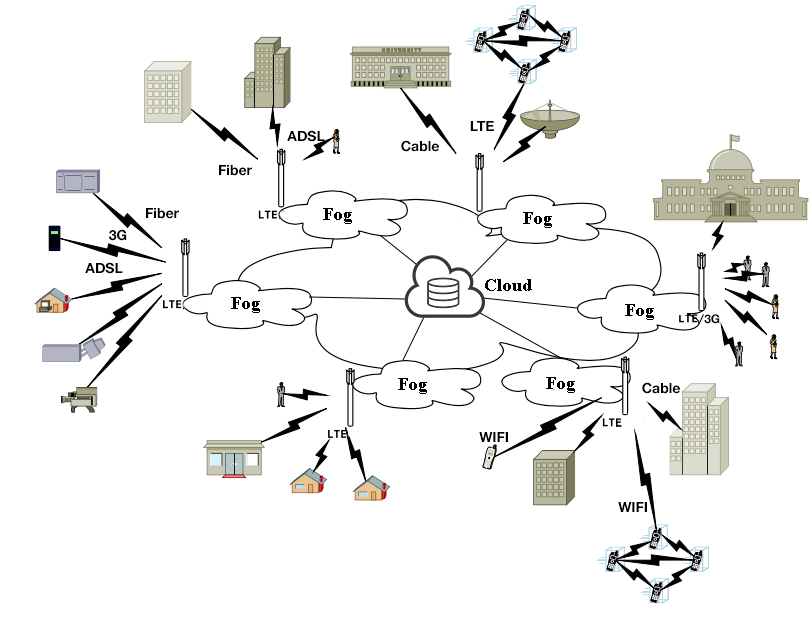
\includegraphics[width=3.5in]{fog-g.png}}
\caption{Typical fog network architecture} 
\label{foggg}
\end{figure}
%

%As shown in \Fig{foggg}, 
%Although, cloud and fog share the same compute, storage and networking techniques, 

%However, planning fog networks can be a complicated task due to the following reasons: %behind fog network planning including but not limited to:
%However, a number of characteristics make the planning of fog networks a non-trivial task.


%However, %Fog Network vendor will then lease their fog infrastructure to different services providers. 
The proximity offered by fog networks addresses the challenges facing today's cloud centre, and enables low-latency IoT applications.
However, when it comes to the planning of fog network, considering the decentralized nature of the fog network combined with a vast number of edge devices, obtaining the optimal network design can be challenging. 
Several factors have to be taken into consideration as follow.
%For instance:
\begin{itemize}
\item Fog facilities need to be highly decentralized.
\item The fog architecture needs to take into account heteromerous hardware requirements.
\item User demands need to be distributed across multiple facilities.
\item The center cloud needs to be able to connect and cooperate with the fog facilities.
\end{itemize}

Unfortunately, a comprehensive survey in the state-of-the-art fog research has noted that the planning and design of fog system deployment has not received any attention so far \cite{mouradian2017comprehensive}. To deal with this problem and provide high-performance fog system design, we propose a mathematical model in this paper, which simultaneously determines the optimal location, the capacity and the number of fog node(s) as well as the interconnection between the installed fog nodes and the cloud. The goal of the model is to minimize the network latency and capital expenditure. To address the multi-objective functions in the problem, one exact algorithm and three approximation algorithms are used and compared in terms of the delay, CPU time and multi-objective quality indicators. 

%With the difficulties mentioned above and the complexity of future networks, service providers need efficient planning tools to implement fog computing networks. 

Essentially, the fog planning problem constitutes two problems, each of them has been proven to be NP-hard:
\begin{itemize}
\item Modular facility location problem
\item Resource allocation problem
\end{itemize}
In addition, from the operator point of view, the objectives of fog planning can be targeted to two conflicting objectives:
\begin{itemize}
\item Minimize capital expenditure
\item Minimize network delay
\end{itemize}

Single-objective optimization is a traditional way of solution in network planning. The designing process is essentially an allocation problem which maximizing the network utility function over a fixed capital expenditure constraint. 
However, in single-objective solution, network designer must use a form of trail and error to try different budget options. The inability to derive an analytically perspective of the problem requires the network designer to execute the single-objective optimization multiple times, thus increasing the computational overhead. 
As opposed to single-objective optimization, multi-objective optimization, we adopt in this work, is more desirable for a network design, due to two major reasons. First, multi-objective optimization techniques attempt to find multiple non-dominated and isolated solutions in a single simulation by emphasizing multiple solutions towards Pareto-front; therefore, speeding up the optimizing process. 
\iffalse
can offer a set of trade-off solutions which are equally optimal, providing sufficient options towards the informed choice that balances all the important objectives. \fi
Second, in network planning, it may be possible, to greatly improve the network performance whilst incurring a very small increase in capital expenditure. Such compromise solutions can be easily missed using single objective method. Therefore, we employ multi-objective optimization in this work to find the optimal set of trade-off solutions and take all the objectives into considerations.
\iffalse
Different multi-objective algorithms have been proposed by previous researchers. For example, the multi-objective fog planning problem can be solved by a linear combination of different objective functions to form a single objective function (weighted sum method) using a commercial solver such as cplex. However, it cannot be solved within a reasonable amount of time due to the NP-hardness.

The multi-objective fog planning problem can be solved by the Evolutionary Multi-objective Optimizations (EMOs)\cite{Deb:2002:FEM:2221359.2221582,smpso}. Since EMOs are heuristic-based algorithms, there is no guarantee in finding Pareto-optimal points \cite{Deb:2001:MOU:559152}. However, EMOs have effective operators to evolve the solution points towards the optimal frontier. For example, in \cite{ITOR:ITOR12294}, the EMO algorithm was proposed to solve the demand scheduling problem, while in \cite{HARRIS20141} the EMO was applied to solve the facility location problem. Therefore, it is interesting to investigate how they perform on the fog network planning problem.
\fi
\iffalse
\section{Background and Motivation}
%\subsection{Fog Related Work}
%Since Cisco[2011] invented the concept of Fog computing (FC). FC has constantly attracted a large number of publications. Researchers started to explore the potential power, services and technologies on fog computing.
Fog computing has been an active area of research due to its potential usage in various scenarios. The characteristics of fog computing have been presented and the characteristics making it the appropriate platform for Internet of Things (IoT) services and applications were discussed \cite{Bonomi:2012:FCR:2342509.2342513, momentum}. The advantage of fog computing over cloud computing, from system perspective, in various IoT and SDN scenario is presented in \cite{fcp}. Fog computing is seen has an horizontal architecture that distributes resources and services of computing, storage, control and networking anywhere along the continuum from Cloud to Things \cite{openfog}. %\cite{momentum} gives a summary of essential features in FC network: wide-spread and geographically available in large numbers, supporting mobility devices and IoT context specialized services. \cite{Vaquero:2014:FYW:2677046.2677052} and \cite{fsurvey} gives comparisons based on different parameters between Cloud Computing (CC) and Fog Computing (FC). 
%\cite{DBLP:journals/corr/Chiang16} discussed seven FC use cases examples: from network content provisioning to client-based HetNets, from shared bandwidth to smart traffic control. 
%\cite{Bonomi:2012:FCR:2342509.2342513} pay attention to how FC add a new dimension to Big Data and Analytics with massively distributed number sources at the edge. \cite{fcsmartcity} envisions the FC in future smart cities and presenting a hierarchical distributed FC architecture to support the massive number of infrastructure and monitoring services

%In \cite{5gcran}, the authors illustrate an analogy technique in 5G with respect to FC: the Cloud RAN technology (CRAN). And authors in \cite{7000980} extend this concept further to Heterogeneous Cloud Radio Access Networks (H-CRAN). See \cite{Peng:2016:FRA:3029494.3029575}, for a complete overview of the concept of this Fog-computing-based RAN.

A Policy-based management of resources in fog computing, which expands the support of secure collaboration and interoperability between different resources is proposed in \cite{secme}. In \cite{fcworkload}, the trade-off between power consumption and transmission delay in the fog computing system has been investigated. The workload allocation problem that aims at minimal power consumption with respect to the constrained service delay has been formulated. \cite{SUN2017687} proposes a fog computing structure to integrate spare resources in the network applying a crowd-funding algorithm.

At the best of our knowledge, the design and planning of fog network has attracted less research activities. The main goal of this paper to fill this gap. We define the Fog Planning Problem (FPP) as a multi-objective problem, where the objective is to minimize the building cost for multiple fog sites and optimize local network performance (e.g., bandwidth and latency) for a given set of constraints (defined in later sections).
%
%\subsection{Single-Objective Optimization Related to Fog Planning Problem}
%The Fog Planning Problem (FPP) is a multi-objective problem. Its objective is to minimize the building cost for multiply fog sites and optimize local network performance (bandwidth and latency). 
%
\iffalse
Intuitively, there are two approaches to model FPP in single objective setting:
\begin{itemize}
\item Minimize the network latency and impose budget constraint (monetary budget, USD). This problem can be modeled as K-median problem.
\item Minimize the building cost of fog infrastructure and impose network latency constraint. This problem can be modeled as Facility Location Problem (FLP)
\end{itemize}
%The first one can be modeled as K-median problem. And the second one can be modeled as Facility Location Problem (FLP).
Though it is tempting to 
Both problem have been deeply researched: K-Median aims to minimize the total distance of each facility and clients with an upper bound on the number of fogs ($K$) that can be opened. Several algorithms have been proposed to solve these problems \cite{Bartal:1996:PAM:874062.875536, Charikar:1999:CAA:301250.301257, Arya:2001:LSH:380752.380755}.

%We use current best Arya et al's local search algorithm as one of comparison. And also there are various heuristic algorithm like: K-means, Spring algorithm and Hot-Spot Greedy algorithm. We also include these algorithm as the comparison. The objective in K-Median is to minimize the total distance of each facility and clients connection. 

Different from K-Median, FLP includes the facility opening and connecting costs into the objective function. Therefore, it reflects the total building budget. The facility location problem has been studied since the 1960s (e.g., Stollsteimer\cite{doi:10.2307/1235442}. It's wide application concerning selecting and placing certain facilities to serve given demand, has always put this problem in a central place in operations research. The first approximation algorithm for the metric incapacitated facility location problem, due to Hochbaum\cite{Hochbaum1982}, achieve $O(\log{}n)$. The first constant factor approximation, 3.16-approximation guarantee was due to Shmoys, Tardos, and Aardal \cite{Shmoys:1997} based on LP-rounding. The current best algorithm, achieving 1.61 guarantee, is due to Jain, Mahdian, and Saberi \cite{Jain:2002}which based on greedy Primal-Dual. What worth mention is, Guha and Khuller \cite{1.43} proved that it is impossible to get an approximation guarantee of 1.463 for the metric facility location problem, unless $NP \subseteq DTIME[n^{O(log{}log{}n)}]$. 
%same reason as before

We use current best Jain et al's algorithm as one of comparison in our simulation and evaluation in following chapter.


\subsection{Multi-Objective Background}
%starting from here
FPP is multi-objective problem (MOP) and solving it requires to optimize two contradictory objectives: minimize total building cost and minimize regional network delay. Different from a single-objective optimization, the main task of MOP is to obtain the Pareto optimal front {\bf{GIVE A REFERENCE}}. 

Suppose, without loss of generality, there are $k$ minimization function $\vec{f}(\vec{x}) = \Big[ f_1(\vec{x}),f_2(\vec{x}), ... , f_k(\vec{x} \Big]^T$ with respect to $m$ constraints $g_i(\vec{x}) \geq 0, i=1,2,..., m$. We need to look for a decision vector $\vec{x} = [x_1, x_2, ..., x_n]$ satisfying all constraints and cannot be improved in any of the objectives without degrading at least one of the other objectives. The set of all these solutions is Pareto optimal.\\

\textbf{Pareto dominance}: A vector $\vec{x^\ast} = (x_1^\ast, ... ,x_n^\ast)$ dominates $\vec{x} (\vec{x^\ast} \succeq \vec{x})$ if and only if $x^\ast$ is not worse than $x$ in all k objectives $(f_i(x^\ast ) \le f_i(x)\ \forall i = 1,..., n)$ and $x^\ast$ is strictly better than x in at least one objective $(f_i(x^\ast ) < f_i(x),\ i = 1,..., n )$.\\

\textbf{Pareto-optimal front} is the set $X$ consisting all non-dominated solutions $x^\ast$ in the search space. Therefore, a solution $x^\ast \in X $, if there is no solution $x \in S$ that dominates $x^\ast$. We call a set of non-dominated solutions that  approximates the Pareto optimal front a Pareto front or known Pareto front.

Theoretically, a Pareto front could contain a large number of points. In practice, a usable solution front only needs to include a limited number of representative points. But they should be as close as possible to the exact Pareto front (convergence) and uniformly spread (diversity) {\bf{GIVE A REFERENCE}}. Because, closeness to the Pareto front ensures that we are dealing with optimal solutions, while a uniform spread of the solutions means that we have made a good exploration of whole search space. Therefore, this Pareto front lets decision maker makes the decision with confidence that no better solution can be achieved without compromise either of objectives. 
%The pursued optimum is a set of solutions known as the Pareto optimal set. 
The Pareto front output is then given to the decision maker, who will choose the best solution according to the real world preferences (like company operational cost or policy requirement).

In FPP, The solutions (Pareto front) should optimize the network delay and building cost simultaneously as in \Fig{plan1}. Each solution should also output the optimal customer allocation respectively as in \Fig{plan1}.
\begin{figure}[h]
\centerline{\includegraphics[width=3.5in]{ttttttttttttt.png}}
\caption{FPP Pareto Front Solution Set} 
\label{plan1}
\end{figure}

As a common sense, a tight budget will affect the network performance. In other words, tight budget building plan, although will still optimize the local service performance, cannot achieve the best network efficiency as ample budget plan, due to limited resources. 

The fog facilities is considered as an abstraction of the machine servers deployed in the network. As can be seen in \Fig{rack}, we can abstract different fog types as each possess different computation resources and capacity to accommodate the user's demands. In real world planning, the number of fog types ($k$) and different fog's profiles can be changed to adequate numbers.
\fi
\subsection{Multi-Objective Combinatorial Optimization Related Work}
The fundamental difference between the multi-objective  and single-objective optimization problems is that, it always aims at optimizing sets of non-dominated solution set, rather than a single optimum \cite{deb2001multi}. The non-dominated means there is no better value improvement that can be made with regard to this objective without degrading another objective. That is to say, these solutions are strictly better in one dimension while no worse than any other dimension. The solution set consisted with all the non-dominated solution holds the most representative within feasible solution space. Evolutionary algorithm (EAs), or more specific, Multi-Objective Evolutionary Algorithms (MOEAs) are ideally suited to multi-objective problems because they produce solutions in parallel through imitating of a natural evolutionary progression (\cite{Deb:2001:MOU:559152}).

The research related to multi-objective optimization can be classified into:
\begin{enumerate}
\item Classical preference-based procedure 
\item Multi-objective evolutionary procedure
\end{enumerate}
In former procedure, it converts a multi-objective problem into a single objective formulation. such as weighted sum approach, compromised approach and rotated weighted metric method\cite{classic}. Or reformulated some objectives as constraints like, $\epsilon$-Constraint method and analytic hierarchy process \cite{MEADE1998201}. Also , there are Benson's method \cite{Benson1998} that drives the solution point to Pareto front through maximizing the difference between solution point and reference point. And Value Function Method that using utility function to guide the search process to preferred objective values. There are also problem oriented algorithm\cite{gen2000genetic} has been proposed. However, their problem-oriented nature, means they cannot be extended to other problems. 

In latter procedure, multi-objective genetic algorithm was used to perform Pareto search\cite{DING2006609} \cite{Bachlaus2008} \cite{cheshmehgaz2013flexible}. Authors in \cite{Villegas2006} presents three algorithms (NSGA-I, PAES and MPEA) to minimize cost and maximize UFLP coverage. Authors in \cite{Deb:2001:MOU:559152} presents a detail description of various MOEAs, and proposed Non-Dominated Sorting Genetic Algorithm II which implement fast ranking function to sped up the search process. We will present a detailed account of evolutionary MO algorithm in section \ref{sec:approximate}
\section{Method for FPP}
The proposed framework solves two kinds of planning scenario: green field scenario (no other facility except cloud) and service expansion scenario (adding regional facilities for increasing demands). The difference is, in former, only cloud is considered as existing facility, but in latter, all existing facility (fogs and cloud) will be labeled as existing before running optimization planning for current phase. In either situation, there will be three steps as can be seen in Fig. \ref{fpphase}. 
\begin{enumerate}
\item Collecting user profile, network status, output user-fog connection matrix.
\item Preprocessing the result from step 1, label unfitted user-fog connection based on policy/environment restriction.
\item Running multi-objective optimizing for fog planning based on user-fog connection matrix, with regarding to cost and network performance objectives 
\end{enumerate}
\begin{figure}[t]
\centerline{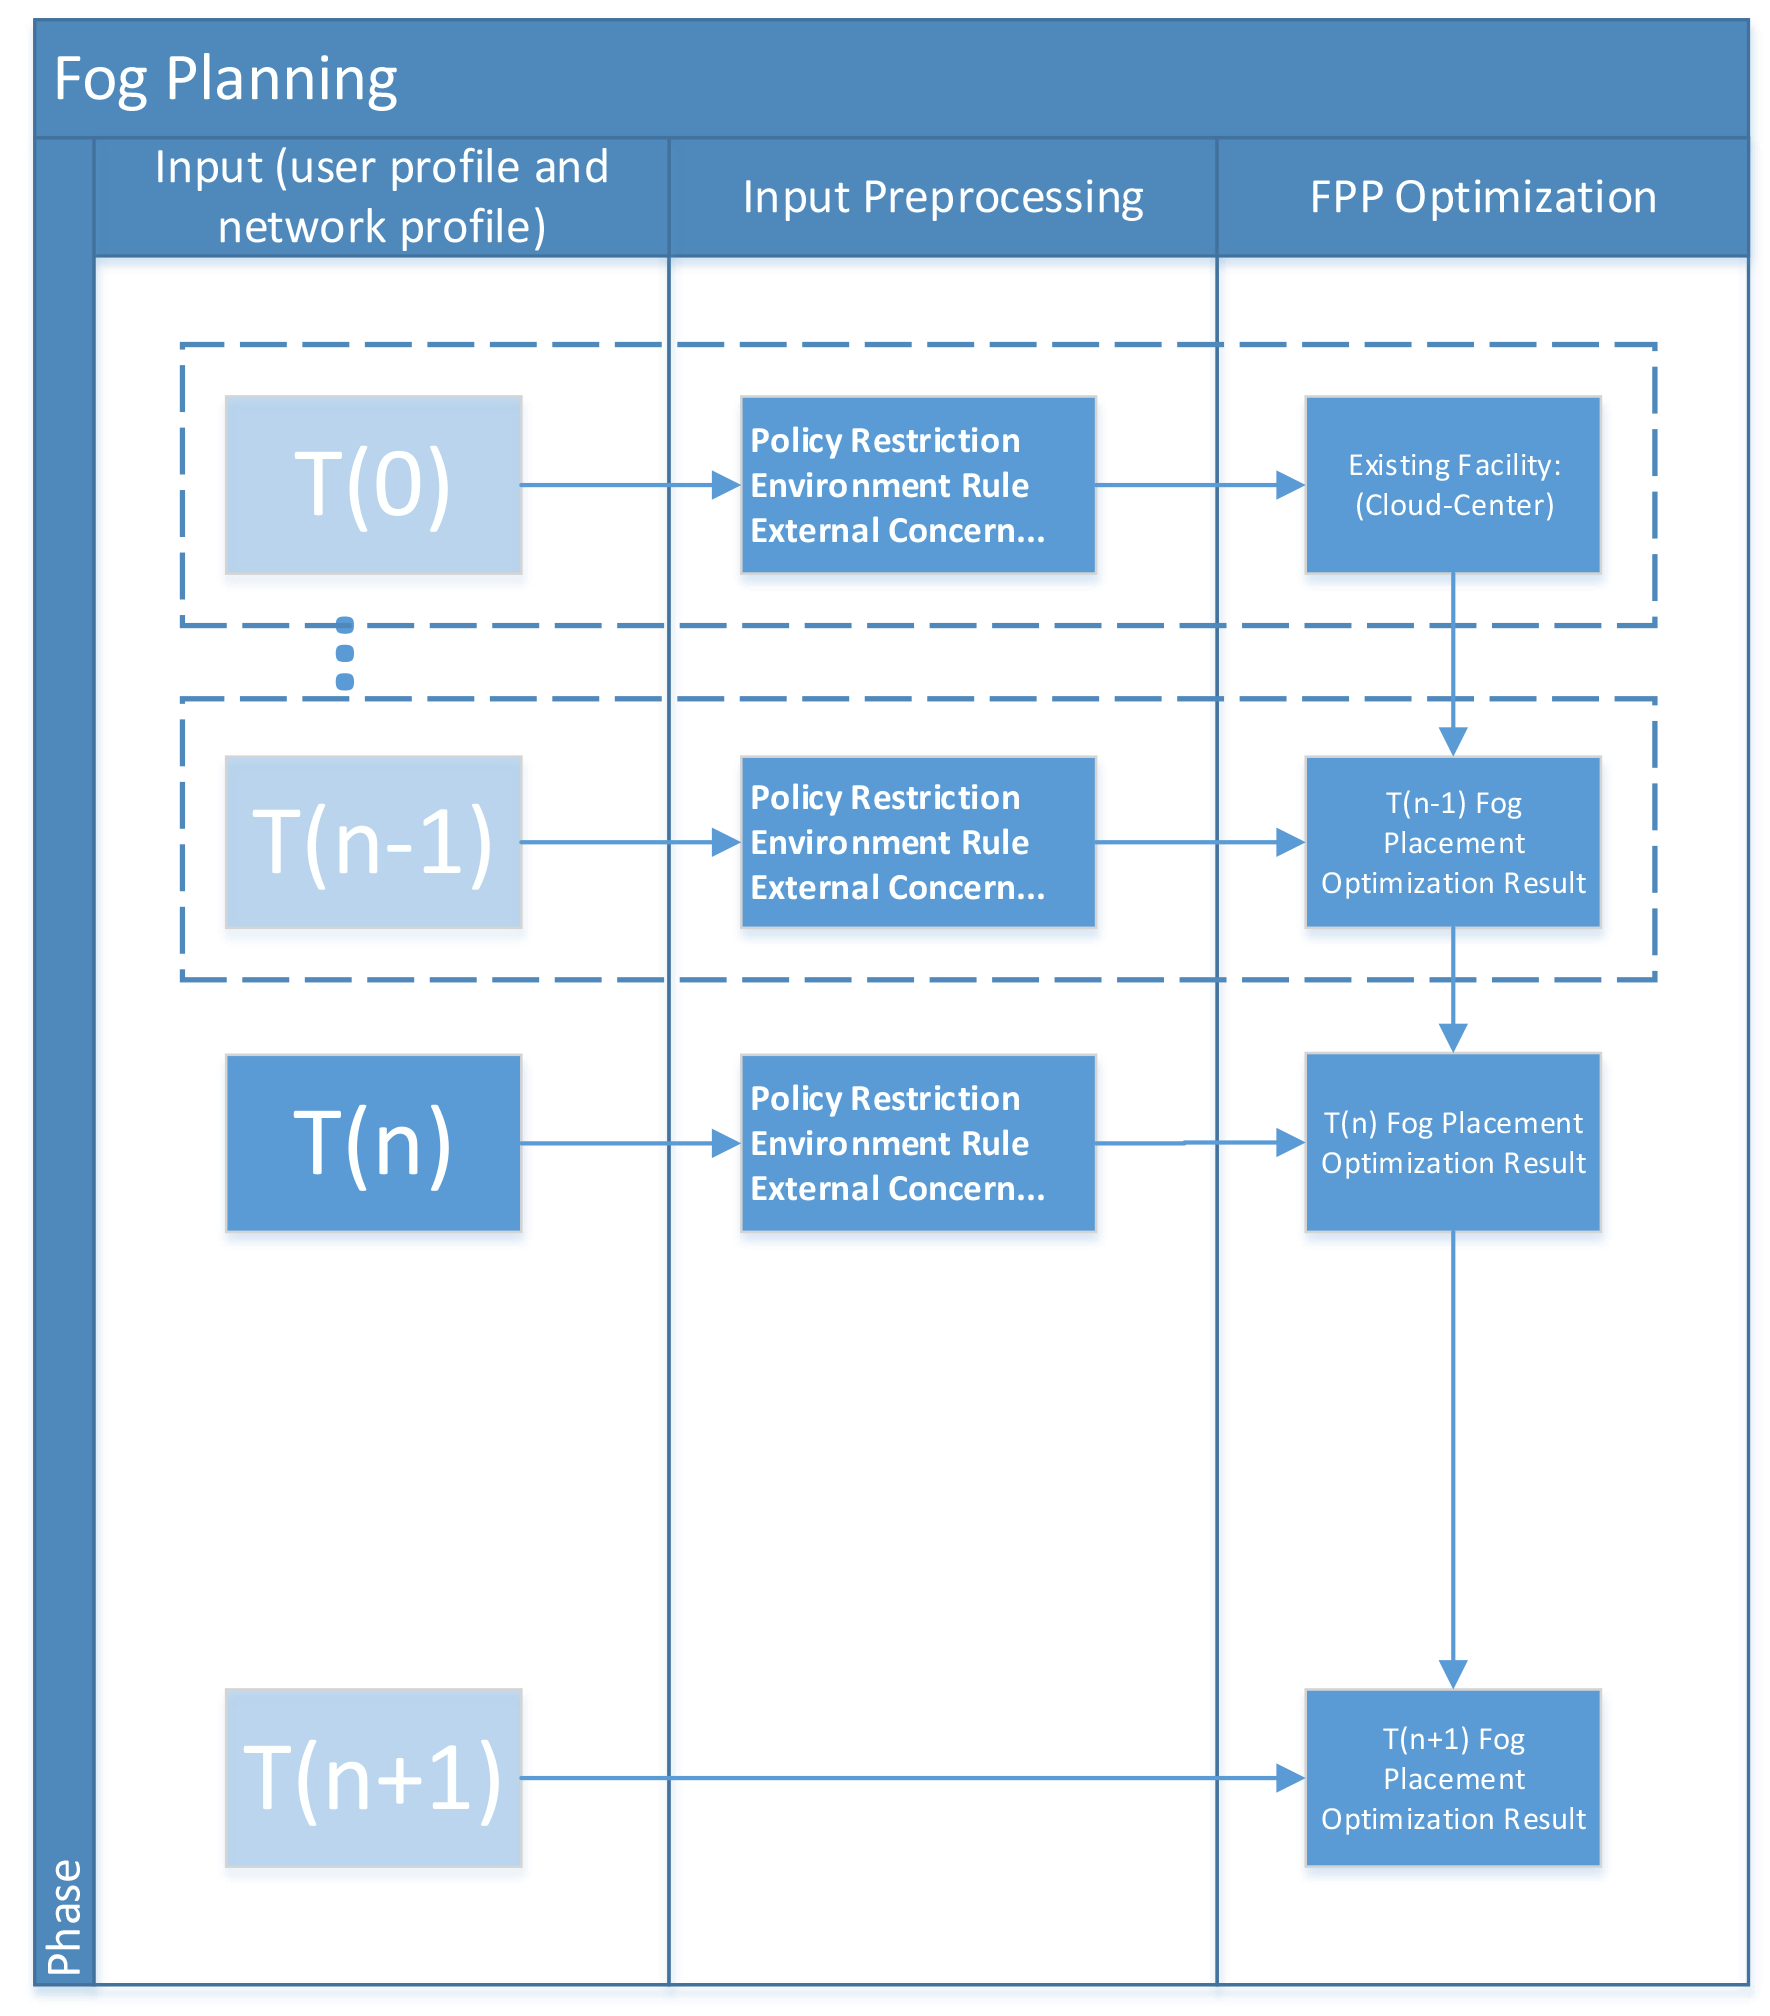
\includegraphics[width=3.0in]{Fogplanningmethod.png}}
\caption{Fog Planning Phases} 
\label{fpphase}
\end{figure}
The optimization in this paper build on the multi-objective work carried out in NSGAII\cite{Deb:2002:FEM:2221359.2221582} and SMPSO \cite{smpso}. The integrated characteristic of multi-objective implies that facility location and user-allocation were combined together. A typical trade-off front solution is illustrated in Fig. \ref{tradeofffront}. The integer string shows which location will be installed with which kind of fog (where 1 represents installing fog type 1, 2 represent type 2, etc. and 0 a closed location). Not only multi-objective model is more straightforward in formulation, but also, we can impose extra constraints based on decision maker's preference and still produce valid solutions with regard to objectives. A common circumstance is, we want to reduce the number of fog installed in this region for management cause, we can easily increase the rental fee or impose a factor $\lambda$, ($ \lambda \geq 1$) on rent. In this way, we increase the proportion of rent cost in associated objective. Therefore, the multi-objective will give solutions with less location open but each open location with much powerful machine. We can observe in Fig. \ref{tradeofffront}, imposing cost factor reduces the total number of fog opened. 
The purpose of this paper is to present a method for exploring trade-off settings in Fog planning. With regard to different network performance, the setting includes fog location, capacity provisioning and user allocation. The decision maker can then use this well-informed and flexible trade-off solutions to make planning decision with confidence no better facility location option left out.
\begin{figure}
\centerline{\includegraphics[width=3.5in]{nov1-fpp.png}}
\caption{Pareto Front Solutions} 
\label{tradeofffront}
\end{figure}
\fi

The remainder of the paper is organized as follows. In Section \ref{probfor}, the Fog Planning Problem (FPP) formulation with dual objective functions is presented. In Section \ref{nphard}, the NP-hardness of the Fog Planning model is analyzed. Section \ref{alfpp} presents a comprehensive explanation of the multi-objective algorithms and optimization procedures. The multi-objective algorithms include the weighted sum method, NSGA-II algorithm, SMPSO algorithm and proposed PSONSGA algorithm. Numerical results are presented in Section \ref{express}, including the evaluation and comparison in terms of the solution quality and computation time. In Section \ref{relwork}, we overview some related works in the area of fog computing and distributed-cloud planning. Finally, conclusions are drawn in Section \ref{conclu}.
\section{Problem Formulation}\label{probfor}
To help understand the problem modelling, we first introduce the following basic concepts.

%\subsection{Basic Concepts}
%\textbf{Fog placement} is the process of selecting a subset of potential locations from a given candidate set and placing fog facilities at these locations.% in order to serve the requests of edge-clusters.

%\textbf{Fog dimensioning} is the process of selecting the capacity levels of fog devices and link types for each candidate site. This selection depends on the node cost, link cost and requirements of edge-clusters' demands.

\textbf{Resource demand: }In this paper, two types of resources are considered at the fog nodes: vCPU cores and memory. 
%For each fog nodes, let $C_{f_i}$ and $ M_{f_i}$ denotes the aggregate request of CPU and memory respectively. It is assumed that fog nodes are provisioned with these two type of resources. 
However, other resources can be included such as the storage and GPU units. This can be achieved by increasing the dimension of the fog profile. For any single period of time, each user-cluster generates a request consisting of vCPU, memory, and bandwidth demands. If a request can be routed to a fog node in such a way that the required vCPU, memory and link bandwidth can be satisfied, then the request is served; otherwise, the request is dropped and sent to the cloud. 

%Given the bipartite graph $G(I, J)$, the objective of the FPP is to, according to the aggregate $C_{f_i}, M_{f_i}$ (CPU demands and memory demands), choose the modular $K$ for each fog centre f and choose the link type $l, (l \in L)$ for each link. Also, each edge cluster $j \ (j \in J) $ should be served by either the fog or the cloud in a sense that the total network usage is minimized. The network usage here can be defined as end-to-end delay or weighted traffic and latency values.
\textbf{Fog type: }The fog type we talk about here is an abstraction of the real-world machine server. Different fog types are associated with different computation resources. In real-world planning, the number of fog types and fog profiles can be changed to adequate types or amounts.

\textbf{Link type: }Similarly, different link types between the fog nodes and the  cloud are considered. Each link is associated with a bandwidth capacity. These links carry the traffic flow between the fog nodes and the cloud for back-end services such as data synchronizations and application management.

\textbf{Edge-cluster: }Edge-cluster is the notion we used to represent an agglomeration of user requests. Typically, several users are using the cloud at the same time from a common geographical region sharing a unique IP prefix. Instead of modelling them individually, we aggregate them together as a ``edge-cluster". However, in optimization research, the request unit is named as ``user". In this paper, the terms ``user'' and ``edge-cluster" have the same meaning.

%\textbf{Edge-cluster routing} can be modelled as an assignment problem. After fog placement and dimensioning decisions are made, an assignment problem must be solved to optimally match edge-clusters with fog facilities.


\subsection{Assumption}\label{assumption}
This section describes the assumptions used in this paper.  
To formulate the fog planning model, we assume the following information is known:  
\begin{itemize}
\item The locations of all the edge devices and the possible locations of all the fog nodes (i.e., $x$ and $y$ coordinates). For each edge device, the generated traffic is known.
\item The characteristics, i.e., memory, virtual Central Processing Unit (vCPU) of different types of fogs that may be installed in the network.
\item The bandwidth availability and the cost of each link type. The link is installed between the fog nodes and the cloud.
\item The cloud has unlimited memory and vCPU. We also assume that the cloud is located in a remote location and if a user cannot be served by the fog, it will be routed to the cloud.
%\item We model the existing computing infrastructures as a set of special fog nodes. These special fog nodes have zero cost and their capacity (memory or vCPU) equals to their available resource capacity. Cloud can be seen as a fog node with zero cost and unlimited capacity. In this way, planning from a green field scenario and expansion scenario can be combined into the same model.
%\item The location of the cloud. We assume that the cloud is located in a remote location and if a user cannot be served by the fog, it will be routed to the cloud.
\item The fog nodes send a fix ratio $\tau$ of their total traffic to the cloud. The $\tau$ here is a tunable parameter. Different applications will have a different value of $\tau$ which captures the amount of traffic that needs to be sent from the fog nodes to the cloud. The possible components of this traffic include database synchronization, data uploading, service management, etc.
\end{itemize}
\iffalse
\begin{figure}
\centerline{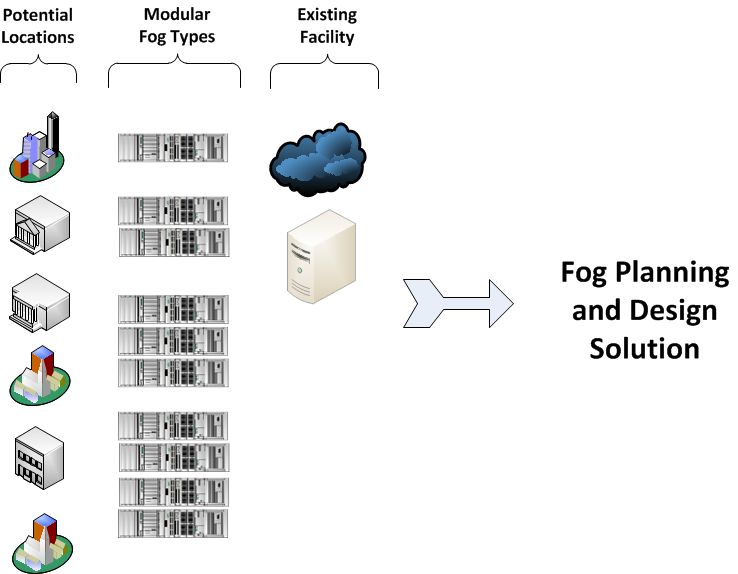
\includegraphics[width=4.5in]{existset.png}}
\caption{Potential Locations, Modular Fog types and Existing Computation Facility} 
\label{exist}
\end{figure}
\fi

%\section{FPP Formulation} \label{sec:fppf}
%In this section, we formulate the fog planning problem as the bi-objective combinatorial optimization problem. Since the building cost and total network delay are equally essential in decision making, defining a bi-objective formula and solving this model in the later chapter is a better option. The bi-objective problem defined here makes sure we have a complete idea of the whole search space of this problem. Therefore, no better option will be left out.




\subsection{Notation}

The following notation is defined based upon the information mentioned above.

\begin{enumerate}
\item Sets
\begin{itemize}
\item $ \textit{I} = \{ 1,...,i,...,m \} $ set of potential location sites. The location $m$ represents the remote cloud-centre.
\item $\textit{J}$, set of edge device clusters that must be served by the fog nodes or the cloud. Each edge-cluster has an aggregated memory, vCPU and traffic demands.
\begin{itemize}
\item $\eta_j$, the total number of vCPU required by an edge-cluster $j \in J$.
\item $\zeta_j$, the total amount of memory required by an edge-cluster $j \in J$.
%\item $\theta_j$, the number of packets requested to the fog nodes or the cloud by a cluster of edge devices $j \in J$
\item $T_j$, the total traffic generated by an edge-cluster $j \in J$.
\item $\kappa_j$, the link speed of an edge-cluster $j \in J$.
\end{itemize}

\item $K$, set of fog types (or capacity level) that can be installed at different locations. Different fog types $k \in K$ have different amount of vCPU, memory.
\begin{itemize}
\item $\alpha^k$ the total number of vCPU available for the fog of type $k \in K$.
\item $\lambda^k$, the total amount of memory available for the fog of type $k \in K$.
\item $c_k^{Fog}$, the cost for a fog of type $k \in K$.
\end{itemize} 
%, different location can have different set of fog type, according to localized space, electricity level and policy restriction.
\item $L$, set of link types that can be installed at different locations to maintain connections to cloud datacenters. Different link types $l \in L$ have different bandwidth capacities. 
\begin{itemize}
\item $\beta^l$, the egress bandwidth upper limit for link type $l \in L$.
\item $c_l^{Link}$, the cost (\$/meter) for a link of type $l \in L$.
\end{itemize}
\item $c_i^{Rent}$, the renting cost for each potential location $i \in I$.
\end{itemize}


%\item $\beta^n$, the number of nodes available for a fog of type $n \in N$


%\item L, set of possible link types that can be used to connect fog nodes and cloud, $L = \left\{l_1, l_2, ...\right\}$  
%\begin{itemize}
%\item $\omega^l$, the bandwidth in Gbps of link type $ l \in L$
%\item $\xi^l$, the price (in dollars per meter) of a link of type $l \in L$  
%\end{itemize}
\iffalse
\item Constants
\begin{itemize}
\item $\sigma$, average packet size (in bytes) sent by the edge devices.
%\item $\tau$, maximum budget (in dollars) allowed for the deployment of the fog.
\item \textit{t}, speed of light (in meters per second).
\item \textit{h}, average number of hops packets take from fog nodes to edge devices.
\item \textit{k}, average processing delay (in seconds) per hop.
\end{itemize}
\fi
\item Functions
\begin{itemize}
\item $d_{ab} = Distance (\textit{a}, \textit{b})$. The euclidean distance between points \textit{a} and \textit{b}. The values of points \textit{a} and \textit{b} are the \textit{x}, \textit{y} coordinates.
\item $\gamma$, processing delay. Each router or switch in the data path adds a finite amount of delay as the packet is received, processed, and then forwarded. This includes the time taken at each layer of the Transmission Control Protocol/Internet Protocol (TCP/IP) down to the bit level layer. The processing delay depends on the hop count between user's connection to fog or cloud. The processing delay is calculated as: 
\begin{align}
\text{Processing Delay} (\gamma) = 
r \cdot h
\end{align}
where $r$ is the mean processing delay for each hop (switch or router) and $h$ represents the hop count.
\item $\psi$, transmission delay. The time taken for a process to send the information to the transmission medium (finer or wire). The transmission delay depends on the link speed that is used and the packet size that is to be sent. The transmission delay is calculated as: 
\begin{align}
\text{Transmission Delay} (\psi) =\sigma / \kappa
\end{align}
where $\sigma$ is the packet size (bytes) and $\kappa$ represents the link speed (bytes/sec).
\item  $\mu$, propagation delay. It equals to the time taken to transmit a signal from the source to the destination. The propagation delay depends on the medium used. For copper wires, the speed can be approximated to 0.59 speed of light. In this paper, we use 0.59 speed of light for the speed of copper wire. The propagation delay is calculated as:  
\begin{align}
\text{Propagation Delay} (\mu) = \frac{d_{ab}}{(0.59 \cdot Light\ Speed)}
\end{align}
where $d_{ab}$ is the euclidean distance between Edge-cluster $a$ and Fog $b$ ($km$). 

\item$D(d_{ab})$. The function $D(x)$ is the network usage descriptor. The network usage function $D(x)$ is an abstraction of the network usage between each user and fog facilities, which could represent the network latency experienced by users or the traffic sending to the cloud. This function is transparent to the optimization algorithm. %We could model users with different classes: guaranteed bit rate (GBR) or best effort (BE). For example, GBR users could be real-time application or latency-sensitive devices, and BE users could be FTP/HTTP download application or periodic synchronization devices which have bandwidth requirement. 
%We use the weighted metric method:
%\begin{align}
%D(x) = (w_1 | f_{delay}(x) - z_{delay}^*|^p + w_2 | f_{traffic}(x) - z_{traffic}^*|^p)^{\frac{1}{p}}
%\end{align}
%The $z^*_{traffic/delay}$ here is the utopia point of traffic or delay value.
%w is non-negative weight. $p \in [1, \infty]$. %The advantage of this method is adjustable w here, can be adjusted to fit customer's preference. z* is the utopian objective value. The distance to utopian points must be normalize before applying $l_p$ norm, which requires knowledge of the minimum and maximum values of traffic/delay\\
In real life planning, latency is arguably the most important performance metric. A small increase in the latency can cause substantial service level degradation \cite{7833029,6678113}. Therefore, in our experiment, the network usage function $D(x)$ is modelled as the point to point delay. 


%The model solution gives the Pareto front of minimal building cost and minimal network delay. If the function $D(x)$ equals to users' outbound traffic to remote cloud. The model gives the Pareto front of minimal building cost and minimal traffic. We can even add different objective function to each Network Usage $D_1(x), D_2(x),...$ for each class of users. In this work, without loss of generality, we model a single Network Usage Objective: end-to-end delay.
%Instead, we use network usage to optimize these two elements together. Therefore, the best total latency and best outbound traffic solution regarding to different cost objective was solved. Next section gives detail on this descriptor.
%\item f(\textit{a},\textit{ b}) is a function that takes the input parameter \textit{a} as the number of packets per second, \textit{b} the packet length in bytes and converts to bytes per second.
%\item g(\textit{a}) is a function that converts a value from Mbps to bytes per second.
\end{itemize}
\item Decision Variables
\begin{itemize}
\item $x_{ij}$,  a 0-1 variable such that $x_{ij} = 1$ if and only if the edge device cluster $j \in J$ is connected to location $i\in I $;
\item $y_{ik}$, a 0-1 variable such that $y_{ik} = 1$ if and only if the fog type $k \in K_i$ is installed at location $i \in I$;
\item $z_{il}$, a 0-1 variable such that $z_{l}=1$ if and only if the link type $l \in L$ is installed at location $i \in I $. 
%\item $v_{uc}$, a 0-1 variable such that $v_{uc} = 1$ if and only if the edge device cluster $u \in U$ is connected to the cloud;
%\item $b_{nl}$, a 0-1 variable such that $b_{nl} = 1$ if and only if the fog node $n \in N$ is connected to the cloud with a link of type $l \in L$;
\end{itemize}
\end{enumerate}
\subsection{Mathematical Model}\label{obj}
Based on the notation presented in the previous section, we can now formulate the Fog Planning Problem, denoted FPP, as follows:

Minimize Cost
\begin{align}\label{obj1}
\textit{Minimize}\bigg[\sum_{i=1}^{m}\sum_{k\in K} y_{ik}c^{Rent}_i +\sum_{i=1}^{m}\sum_{k\in K}  y_{ik} c^{Fog}_k +\\
\sum_{i=1}^m \sum_{l\in L} z_{il} c^{Link}_l d_{i,cloud}\bigg]
\end{align}

Minimize Delay 
\begin{align}\label{obj2}
\textit{Minimize} \bigg[\sum_{i=1}^m\sum_{j\in J} D(d_{ij}) x_{ij}\bigg]
\end{align}
$$
D(d_{ab})  = 
	\begin{cases}
	\begin{aligned}
	&\psi^{ToFog} + \mu^{ToFog} + \gamma^{ToFog}&\sum_{i \in I  \setminus m}x_{ij} =1\\
	 &\textbf{ (connect to the fog)}\\
	&\psi^{ToCloud} + \mu^{ToCloud} + \gamma^{ToCloud}&x_{mj} = 1\\
	& \textbf{ (connect to the cloud)}\\
	\end{aligned}
	\end{cases}
$$
As shown above, to achieve the maximum network performance and cost efficiency, the model simultaneously minimizes the total network delay and the total capital expenditure required to deploy the fog network.  %and the amount of traffic sent to the cloud..\\

Both Equation \Eq{obj1} and Equation \Eq{obj2} are subject to following constraints:
\begin{align}
&\sum_{i=1}^m x_{ij} =1\quad  (\forall j \in J )\label{st1}
\end{align}
Constraints \Eq{st1} are the single source constraints. They ensure that each user connects to exactly one fog or cloud. \\
\begin{align}
&\sum_{k\in K} y_{ik} \leq1 \quad(\forall i \in I )\label{st2}
\end{align}
Constraints \Eq{st2} are the uniqueness constraints. They enforce that at most one fog node is installed at a given location.  In practice, we can install multiple servers in each location, and each server can have different hardware configurations (memory sticks, CPU, hard disk drive, GPU, etc.) To reduce the complexity, we generalize different server types and hardware combinations to a fix number of fog types. Under this assumption, each potential location can select an appropriate fog type to accommodate the workload demands. In other words, we cannot install two or more fog nodes at the same location. If the left side of Equation \Eq{st2} equals to zero, it means that the corresponding location is not selected; no fog facility will be installed at this location.\\
\begin{align}
&\sum_{l\in L} z_{il} \leq1\quad(\forall i \in I) \label{st22}
\end{align}
Similar to Constraints \Eq{st2}, Constraints \Eq{st22} are the link uniqueness constraints. They enforce that at most one link type can be installed at each location. If Equation \Eq{st2} equals to zero, the corresponding location is not open and therefore, no link will be installed at this location.\\
\begin{align}
& x_{ij} - \sum_{k\in K} y_{ik}\leq0  \quad(\forall i \in I,\forall j \in J)\label{st3}
\end{align}
Constraints \Eq{st3} : Openness constraints. These constraints ensure that users can only connect to a fog that is opened.\\
\begin{align}
&\sum_{l\in L} z_{il} \leq \sum_{k\in K} y_{ik} \quad (\forall i \in I) \label{st23}
\end{align}
Constraints \Eq{st23} make sure that each installed fog node at location $i$ will be connected to the cloud.\\
\begin{align}
&\sum_{j\in J} \eta_j x_{ij} \leq \sum_{k\in K} y_{ik}\alpha^k \quad(\forall i \in I)\label{st4}
\end{align}
\begin{align}
&\sum_{j\in J} \zeta_j x_{ij} \leq \sum_{k\in K} y_{ik}\lambda^k \quad(\forall i \in I)\label{st41}
\end{align}
Constraints \Eq{st4} and \Eq{st41} are the capacity constraints. They are the capacity constraints for vCPU, memory at the node level. They ensure that the total resource demand does not exceed each fog node's hardware capacity. %Noticeably, since the demands and capacity parameters can only be positive. Constraints \Eq{st4} render the Constraints \Eq{st3} to be unnecessary. So we omit the Constraints \Eq{st3} in following formulations and experiments.\\
\begin{align}
&\sum_{j\in J} x_{ij} T_j \cdot \tau \leq \sum_{l\in L} z_{il} \beta^l\quad(\forall i \in I) \label{stl}
\end{align}
Constraints \Eq{stl} are the link capacity constraints. They state that the total bandwidth from fog site to cloud cannot exceed the egress link bandwidth upper bound.\\
\begin{align}
&x_{ij} \in \{0,1\} \quad (\forall i \in I, \forall j \in J)\label{st5}\\
& y_{ik} \in \{0,1\} \quad (\forall i \in I, \forall k \in K)\label{st6}\\
& z_{ik} \in \{0,1\} \quad (\forall i \in I, \forall k \in K)\label{st7}
\end{align}
Finally, Constraints \Eq{st5}, \Eq{st6} and \Eq{st7} define the decision variables as binary.
\section{NP-Hardness}\label{nphard}
This section establishes the NP-hardness of the FPP.
The FPP has two objective functions that need to be minimized: building cost and network delay. The decision variables consist of the placement and assignment decisions. % such as where to install fog facility, which type of fog should be installed, which type of link should be installed and which facility should serve a particular customer. 

Essentially, this problem is a multi-objective combinatorial problem. If we relax certain conditions, there are related single-objective optimization problems that we can gain insight from.
Suppose that we know that certain number of fog facilities will be opened and that we relax the capacity constraint at each location. Then the problem of assigning edge-clusters to open facilities while minimizing the total delay can be reduced to the K-median clustering problem.

\textbf{K-median clustering problem}: Suppose there exists a bipartite graph with a bi-partition (F, C), where F is a set of facilities and C is a set of clients, and let $k$ be a positive integer specifying the number of facilities allowed to be opened. Let $c_{ij}$ be the cost of connecting client $j$ to facility $i$. The objectives are to find a subset $I \subseteq F, |I| \leq k$ of facilities that should be opened and a function $\phi: C \to I$ assigning clients to open facilities that minimize the total connecting costs \cite{Vazirani:2001:AA:500776}.

The NP-hardness of the K-median clustering problem was proved in 1984 by Megiddo and Supowit \cite{1984}. 
%The current best approximation algorithm is due to Arya et al. \cite{Arya:2001:LSH:380752.380755}, which is a local search algorithm.
However, even if we can solve this problem using an approximation algorithm, we still have to decide a reasonable $k$ regarding to the total budget. %Moreover, there is no capacitated constraint on each fog site, which makes this model an oversimplification of the FPP model.

From another perspective, suppose we combine the building cost and network delay into a single objective function. The objective function becomes:
\begin{align}
\textit{Minimize}: \ \alpha\cdot\overset{opened\ fog}{\sum} \textit{fog building cost} + \\
\beta \cdot \overset{all\ users}{\sum}\textit{network delay}
\end{align}
where $\alpha$ and $\beta$ are the normalizing constants.
%Since in our problem, each fog site has a capacity upper limit. 
Problems of this form are referred to as the capacitated facility location problem.\\


\textbf{Capacitated Facility Location 
Problem (CFLP)}: Suppose there exists a bipartite graph with a bi-partition (F, C), where F is a set of facilities and C is a set of clients. A fixed cost $f_i \geq 0 $ for opening each facility $i \in F$; a capacity $u_i \geq 0 $ for each facility $i \in F$; a demand $d_j \geq 0$ for each client $j \in C$. The problem is to find a subset $I \subseteq F$, of facilities to opened as well as a assignment function $\phi: C \to I $ that assigns clients to open facilities. The objective is to minimize the total connecting cost without violating each facility's capacity constraint: $\sum_{j \in C} x_{ij} d_j \leq u_i,  \forall i \in F$ \cite{Vazirani:2001:AA:500776}. 

Megiddo and Supowit  \cite{1984} proved that exact solution of CFLP is NP-hard. Fowler el al. \cite{FOWLER1981133} proved that when the error is small, even a approximation to this problem is NP-hard.
%Most known approximation algorithms for CFL are based on local search techniques since the standard LP relaxation has an unbounded integrality gap for the general case. The current best approximate method due to Bansal et al \cite{Bansal:2012:CFL:2404160.2404173}, which achieve approximate ratio of 5.

Specifically, our problem needs to add a single source constraint. The reason is each users can only go to one single fog; in this regard, the problem becomes the Single-Source Capacitated Facility Location Problem (SSCFLP). In SSCFLP, deciding whether a feasible solution exists at all is NP-complete \cite{bonn}.
Moreover, our problem has a modular facility cost model, which provides several capacity levels of the fog facility. This transfers the model to a single-source modular capacitated facility location problem, which is a more complicated version of CFLP \cite{bonn}.

As discussed above, the single objective model of this problem is extremely complicated and computational complex. Therefore, in the following sections, we will introduce methods to solve this planning problem from the multi-objective perspective.

\section{Algorithm for FPP}\label{alfpp}


\subsection{Exact Algorithm for FPP}
To solve the multi-objective problem. The directed thinking approach is to combine multiple objectives into one single objective. The Weighted Sum Method applied to this ideology.
\subsubsection{Weighted Sum Method}
The weighted sum approach combines multiple objective functions into a single objective function. In this combination, different objectives are given a certain weight between 0 and 1. The multi-objective problem can be combined by using the Formula \Eq{wsequation}.
\begin{align}%\label{ws}
&min\ or\ max \bigg\{\sum_{j=1}^Q \lambda_j z^j (x) : x \in X \bigg\}\label{wsequation}\\
&0\leq \lambda_j \leq 1\\
&\sum_{j=1}^Q \lambda_j = 1
\end{align}
where $\lambda_j$ is the weight parameter assigned to each objective to capture the relative importance on a given objective. Assigning a higher (lower) weight places more (less) emphasis on this objective.
\subsection{Approximate Algorithm for FPP}\label{sec:approximate}
In this paper, the Evolutionary Multi-objective Optimization (EMO) is applied to solve the fog planning problem. EMO is based on heuristic multi-objective optimization techniques that imitate the principles of natural selection and survival of the fittest to find near-optimal solutions [23]. In EMO, multiple Pareto-optimal solutions are found in a single simulation by emphasizing multiple non-dominated and isolated solutions [23].
The experiment result shows that neither NSGAII nor SMPSO is capable to produce solid result with strict convergence and rich coverage. Therefore, we propose PSONSGA algorithm to overcome the drawbacks of either these algorithm. The experiment in next section shows our algorithm outperforms NSGAII and SMPSO in coverage and convergence respectively.

\subsubsection{Non-dominated Sorting Genetic Algorithm II}
NSGA-II follows the same steps as the classical GA. The classical GA first initializes a population of \textit{N} individuals, then it generates offsprings by applying the crossover and mutation operations, and finally evaluates and selects the fittest solutions as output solutions. What differentiates NSGA-II from previous algorithms (such as VEGA and HLGA) is an intuitive invention of the fast elitist ranking procedure (Non-dominated Sorting). Using this fast ranking procedure, NSGA-II always preserves the best (higher rank in non-dominated rank and larger crowding distance) solutions inside the latest population. 
The pseudocode of the NSGA-II algorithm is presented in Fig \ref{nsga2}.
\begin{figure}[h]
\caption{NSGA-II Algorithm}
\indent\fbox{%
\begin{minipage}{\dimexpr\linewidth-2\fboxsep-2\fboxrule\relax}
\quad
\begin{algorithmic}[1]
%\Procedure{MyProcedure}{}

\STATE Initialize a population of $N$ individuals as the ``parent population" P 
\WHILE{\texttt{Iteration $<$ MaxIteration}}
	\STATE \textit{C} $\gets$ Empty\ child\ population
	\WHILE{\texttt{the number of individuals \textit{C} in <  $N$}}
	\STATE Select\ parent1 (by\ tournament\ selection)
	\STATE Select\ parent2 (by\ tournament\ selection)
	\STATE Get child1, child2 through the Binary Crossover (parent1,\ parent2)
	\STATE Polynomial\ Mutation (child1, child2)
	\STATE Evaluate\ child1, child2\ for their fitness values
	\STATE Insert\ child1,\ child2\ into\ \textit{C}
	\ENDWHILE
	\STATE \textit{U} $\gets$ Combine\ \textit{P}\ and\ \textit{C}\ to\ get\ \textit{2N}\ individuals
	\STATE Rank\ the\ union\ set\ \textit{U}\ using\  the non\-dominated\ sorting. %(As\ explained\ in\ \ref{nds})
	\STATE \textit{P} $\gets$ \textit{N}\ front\ individuals\ in\ \textit{U}\ by\ the crowded\ comparison\ selector. %(As\ explained\ in\ \ref{cdc})
\ENDWHILE
\STATE Return the set of feasible non-dominated solutions in the latest population.
%\EndProcedure
\end{algorithmic}
\label{nsga2}
\end{minipage}% 
}
\end{figure}

\iffalse
\begin{figure}[h]
\caption{NSGA-II Algorithm}
\noindent\fbox{%
\begin{minipage}{\dimexpr\linewidth-2\fboxsep-2\fboxrule\relax}
\quad
\begin{algorithmic}[1]
%
%\Procedure{MyProcedure}{}
\STATE $\textit{n} \gets \text{Population size}$
\STATE $P \gets$ Initialized parent population by randomly 
creating n individuals
\WHILE{\texttt{Iteration $<$ MaxIteration}}
	\STATE C $\gets$ Empty\ child\ population
	\WHILE{\texttt{not enough individuals in C}}
	\STATE Select\ parent1 (by\ tournament\ selection)
	\STATE Select\ parent2 (by\ tournament\ selection)
	\STATE Getting child1, child2 through Simulated Binary Crossover(parent1,\ parent2)
	\STATE Polynomial\ Mutate (child1, child2)
	\STATE Evaluate\ child1, child2\ for\ fitness
	\STATE Insert\ child1,\ child2\ into\ C
	\ENDWHILE
	\STATE U $\gets$ Combine\ P\ and\ C\ to\ get\ 2n\ new\ individuals
	\STATE Rank\ the\ union\ set\ U\ by\ non\-dominated\ sorting.
	\STATE P $\gets$ n\ front\ individuals\ in\ U\ by\ crowded\ comparison\ selector. 
\ENDWHILE
\STATE Return the set of feasible non-dominated solutions in the latest population.
%\EndProcedure
\end{algorithmic}
\label{nsga2}
\end{minipage}% 
}
\end{figure}
\fi

\subsubsection{Speed-Constrained Multi-Objective Particle Swarm Optimization}
Particle Swarm Optimization (proposed by J. Kennedy and R. Eberhart in \cite{poli2017}) models the social behaviour of biological creatures through the mathematical approach.

The pseudocode of the SMPSO algorithm is presented in Algorithm \ref{SMPSO}.
Similar to the classical PSO algorithm, SMPSO first randomly generates a set of \textit{N} initial solutions, then iteratively updates the ``solution positions" in the searching space \cite{smpso}.
In each iteration, every particle adjusts its velocity to follow the local and global best solutions. We assume that each particle $i$ is randomly assigned a position $\vec{x}_i\ (i=1, 2, ..., N)$ and a velocity $\vec{v}_i\ (i=1,2,...,N)$. The algorithm updates the particle's position by:
\begin{equation}\label{psoposition}
\vec{x}_i(t) = \vec{x}_i(t-1) + \vec{v}_i(t)
\end{equation}
The velocity function $\vec{v}_i(t)$ is given by:
\begin{equation}\label{psospeed}
\vec{v}_i(t) = w \cdot \vec{v}_i(t-1) + C_1 \cdot r_1 \cdot (\vec{x}_{p_i}- \vec{x}_i)+ C_2 \cdot r_2 \cdot (\vec{x}_{g_i} - \vec{x}_i)
\end{equation}
where $\vec{x}_i(t)$ and $\vec{v}_i(t)$ are the location and velocity of particle \textit{i} at time \textit{t}. 
The $\vec{x}_{p_i}$ and $\vec{x}_{g_i}$ are respectively, the historical best and the global best points.
$w$ is the inertia weight of the particle, which controls the trade-off between the global and local experience.
$C_1$ and $C_2$ are learning factors which control the effect of the local and global best particle.
$r_1$ and $r_2 $ add randomness between the global and local searching direction.
%Instead of putting all solution within same ``swarm population", SMPSO maintains another ``elite archive", in which only stores non-dominated solution with highest crowding distance. 
%Different from genetic algorithm, all the global points in speed computing process are selected from this ``archive population". SMPSO also applies mutation operation upon part of the swarm population in order to diversify the swarm solutions.

\begin{figure}[h]
\caption{SMPSO Algorithm}
\indent\fbox{%
\begin{minipage}{\dimexpr\linewidth-2\fboxsep-2\fboxrule\relax}
\quad
\begin{algorithmic}[1]%\Procedure{MyProcedure}{}
\STATE Initialize a population of \textit{N} individuals as ``swarm population" \textit{S} 
\STATE Evaluate the solutions in the ``swarm population"
\STATE Put non-dominated solutions into an empty ``elite archive" \textit{A} 
\WHILE{\texttt{Iteration $<$ MaxIteration}}
	\FOR{$s \in S$}
		\STATE Use constrained binary tournament to select a solution from the elite archive
		\STATE Use the solution from last step as the global best particle
		\STATE Compute the speed of \textit{s} according to the speed formula \Eq{psospeed}
		\STATE Update the position of \textit{s} according to the speed calculated in the last step
	\ENDFOR
	\STATE Apply the polynomial mutation to $\tau \%$ of the population
	\STATE Evaluate the solutions in the swarm population 
	\STATE Insert the non-dominated solutions from $S$ to $A$.
\ENDWHILE
\STATE Return the set of feasible non-dominated solutions in the elite archive ($A$).
%\EndProcedure
\end{algorithmic}
\label{SMPSO}
\end{minipage}% 
}
\end{figure}



\subsection{Proposed EMO Algorithm (PSONSGA)}
Previous studies in NSGA-II and SMPSO mainly focus on applying these algorithms on continuous problems. 
However, for discrete problems, such as the combinatorial problem we are dealing with, the preliminary results of our experiment reveal that these two heuristic algorithms hold different characteristics.% compared to their counterparts in continuous domain.

As shown in \Fig{nsgalabel}, the NSGA-II performs efficiently regarding the convergence to the Pareto front, however, its solution points are unevenly distributed in the search space.  Even if we change the mutation index or the crossover index settings, no obvious improvement can be perceived. The researchers in 
\cite{doi:10.1163/156939308784160703}, have observed the same disadvantage in continuous NSGA-II applications. This disadvantage stems from the NSGA-II's sorting process. The concentrated effect in the non-dominated sorting harms the diversity in NSGA-II solutions. % as can be seen in \Fig{nsgauneven}.
\iffalse\begin{figure}[H]
\centerline{\includegraphics[page=1,width=5.in]{nsgauneven.png}}
\caption{The diversity is influenced by the concentrated sorting process \cite{doi:10.1163/156939308784160703}} 
\label{nsgauneven}
\end{figure} 
\fi
The researchers in \cite{doi:10.1163/156939308784160703} proposed an elitism strategy to overcome this shortcoming. However, the time-complexity involved in evaluating the elitism sets is high, and can be a huge issue for large scale problems.
\begin{figure}[h]
\centerline{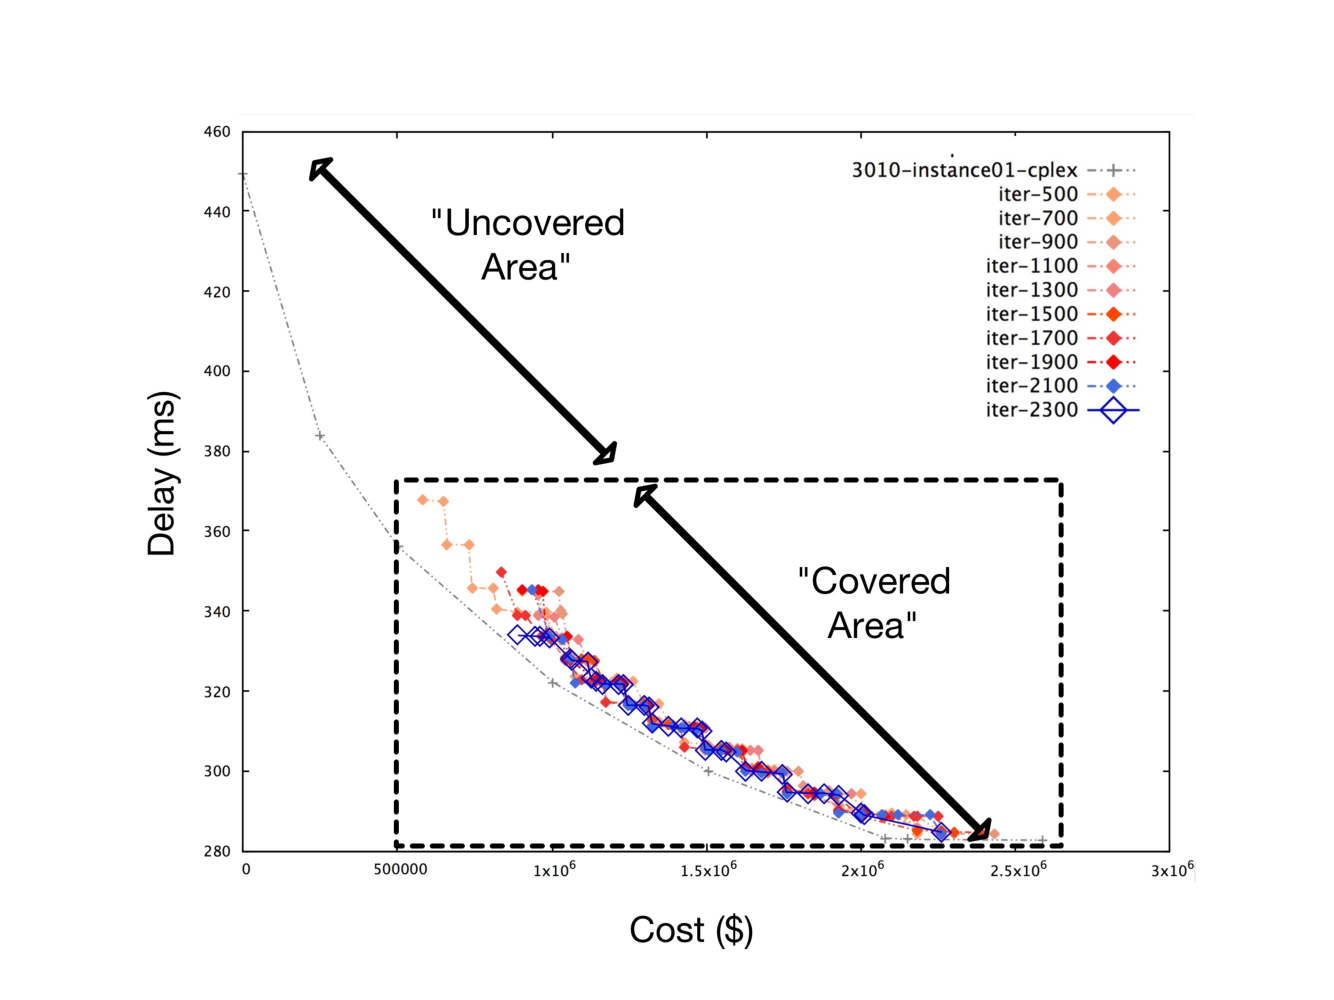
\includegraphics[page=1,width=3.5in]{nsgaitertest_label.pdf}}
\caption{NSGA-II algorithm struggles to cover the whole Pareto front} 
\label{nsgalabel}
\end{figure} 
%, the reason behind this, is how genetic algorithm work. Even though some mutation individual may goes to the uncharted area in middle of iteration, this aspiration point at infant statues will give worse objective function value compare to main-stream points. The Genetic algorithm will only keep certain amount of good result to new round of iteration. It will be difficult for these special points to survive.

On the other hand, SMPSO shows different characteristics. The preliminary experiment demonstrates that SMPSO performs efficiently on exploring the whole front. It preserves the diversity in the solutions set and always produces evenly distributed Pareto frontiers. However, after a given number of iterations, SMPSO struggles to push the solution set to converge to the true optimal front. 
The preliminary results are shown in \Fig{smpsolabel}.
%The reason is the way SMPSO search scheme works seems has trouble go to the global optimal. My analogy is that ant search for food. They good at find new search direction, but not good at converge to the global best route.
\begin{figure}[H]
\centerline{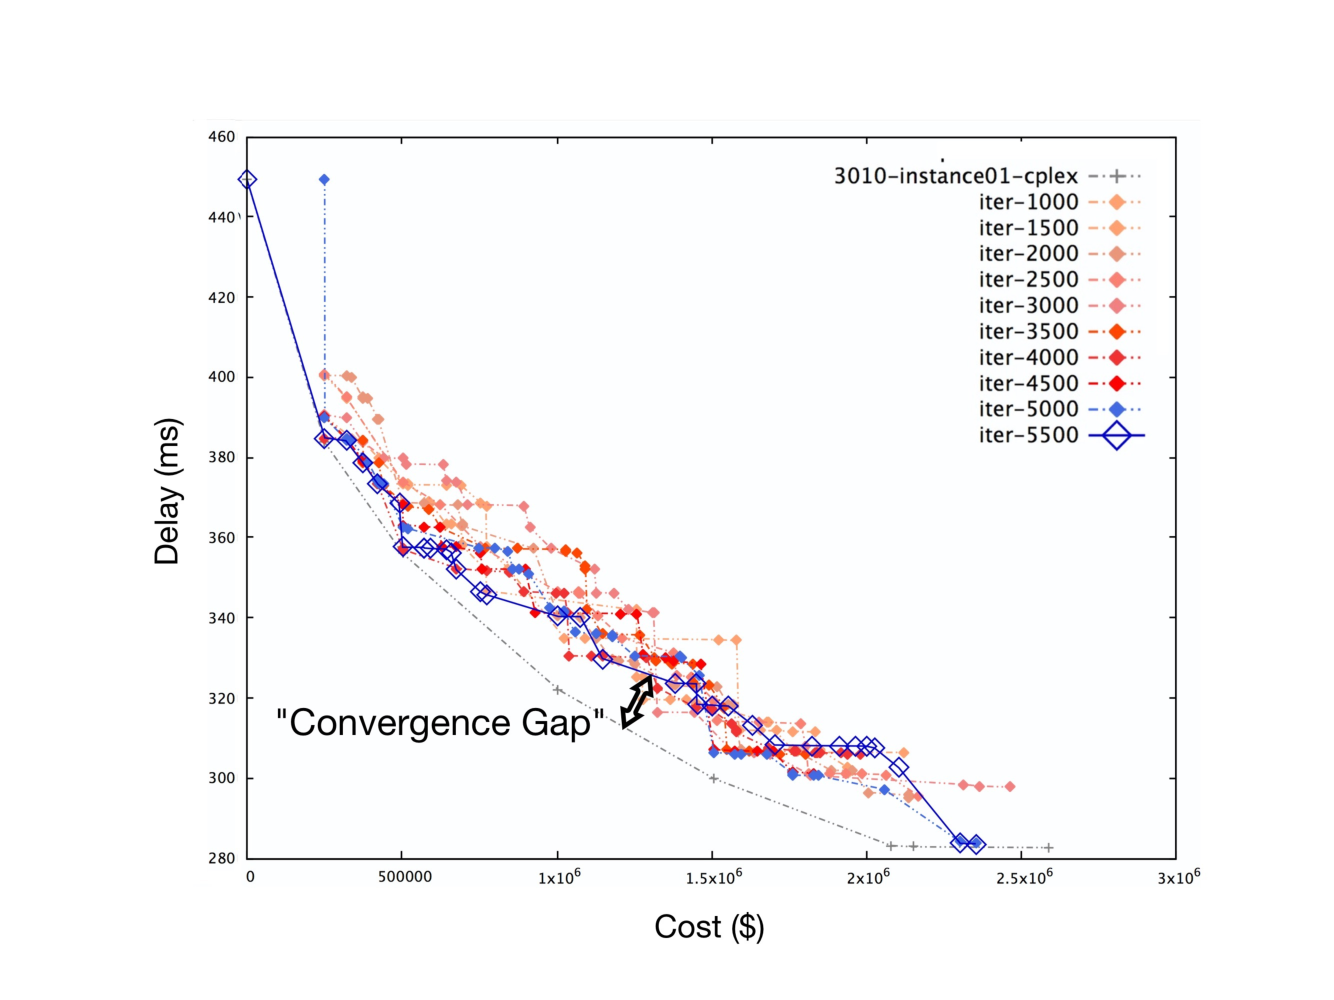
\includegraphics[page=1,width=3.5in]{SMPSO_iterationtest_label.pdf}}
\caption{SMPSO algorithm struggles to converge to true pareto front} 
\label{smpsolabel}
\end{figure}

Motivated by the disadvantages in NSGA-II and SMPSO algorithms, we propose a new version of NSGA-II. The algorithm developed is named Particle Swarm Optimized Non-dominated Sorting Genetic Algorithm (PSONSGA). The PSONSGA is designed specifically to exploit the searching efficiency of PSO-based algorithms.
 %Instead of introducing extra time-complexity, like the elitism strategy or other enforcement fitness function or evaluation function in \cite{Fortin:2013:RNC:2463372.2463456}. 
%In this paper, we employ the SMPSO preprocess procedure in our PSONSGA algorithm%.
%Therefore, we propose PSONSGA algorithm to solve the FPP. 
Particle Swarm Optimized Non-dominated Sorting Genetic Algorithm~(PSONSGA) is a variation of NSGA-II based on the idea of employing particle swarm optimization before proceeding to the NSGA-II's procedure. Following the similar two-phase methodologies in \cite{magnier2008multiobjective,onut2008two,sabri2000multi}, PSONSGA consists two optimizing phases: the PSO phase and the NSGA-II phase. The purpose of the PSO phase is to explore the decision space and preserve the diversity in the solution population. In the NSGA-II phase, the non-dominated sorting emphasizes the effort to converge the solutions towards the optimal front. Furthermore, in the NSGA-II phase, an enforced selection process is introduced to increase the fitness pressure on the population.
The pseudocode of PSONSGA is presented in Algorithm~\ref{PSONSGA}. 
PSONSGA uses the same behaviour as in the SMPSO for the first 50\% of the run. In the last 50\% of the run, a variant of NSGA-II with an aggressive selection is executed.
The aggressive selection enforces the convergence of solutions and the extension of the solution front. The population is expected to get closer to the optimal solutions.
%\textbf{rewrote}
% The main idea of PSONSGA algorithm is to first using PSO algorithm to search the whole area, and then feed this mid-term solution into NSGA-II runner. Then let NSGA-II evolve this point to Pareto Front. 
 \subsubsection{Procedures of PSONSGA}
\textbf{PSO procedure}
In the first 50\% of the PSONSGA iterations, the PSO procedure is employed to explore the decision space, and to test different search directions (see rows 3-12). The position and velocity updating mechanism in PSO, speeds up this searching process. The diversity in population is preserved before proceeding to the next phases. 
\textbf{NSGA-II procedure}
In the last 50\% of the run of PSONSGA, the population is expected to be evenly diversified and relatively close to the Pareto front. The main goal is not to explore the searching space anymore but to increase the closeness to the optimal solutions (see rows 17-27) \cite{concordia}. The NSGA-II procedure, including non-dominated sorting, is executed to concentrate the solutions towards the true optimal front. Also, we employ an aggressive selection process as proposed in \cite{concordia} (see row 24).
\begin{figure}[h]
\caption{PSONSGA Algorithm}
\indent\fbox{%
\begin{minipage}{\dimexpr\linewidth-2\fboxsep-2\fboxrule\relax}
\quad
\begin{algorithmic}[1]

\STATE Initialize a population of \textit{N} individuals as ``swarm population" $S$
\STATE Evaluate the solutions in the $S$
\STATE Put non-dominated solutions into an empty ``elite archive" \textit{A} 
%\While{\texttt{Iteration $<$ MaxIteration\_Alpha}}
%\Do
\WHILE{\texttt{iteration $\le$ 50\% Maximum iteration}}
	\STATE \textbf{PSO procedure:}
	\FORALL{$s\in S$}
	\STATE Use constrained binary tournament to select a solution from elite archive
	\STATE Use the solution from last step as the global best particle
	\STATE Compute the speed of $s$ according to the speed equation shown in \Eq{psospeed}
	\STATE Update the position of \textit{s} by the speed calculated in the previous step
	\ENDFOR
	\STATE Apply the polynomial mutation to 15\% of the population
	\STATE Evaluate the solutions in the swarm population 
	\STATE Update the elite archive: insert the non-dominated solution from swarm to archive 
\ENDWHILE

\STATE \textit{M} $\gets$ Elite solutions in SMPSO's elite archive $A$
\STATE \textit{C} $\gets$ \textit{M} (Use the solutions in \textit{M} as initial population for NSGA-II)
\WHILE{\texttt{Iteration $\le$ MaxIteration}}

	\STATE \textbf{NSGA-II procedure:}
	\STATE \textit{D} $\gets$ Empty\ child\ population
	\STATE Use constrained binary tournament to select parents in \textit{C}.
	\WHILE{\texttt{not enough individuals in \textit{D}}}
	\STATE Select\ parent1 (by\ tournament\ selection)
	\STATE Select\ parent2 (by\ tournament\ selection)
	\STATE Getting child1, child2 through Binary Crossover (parent1,\ parent2)
	\STATE Polynomial\ Mutation (child1, child2)
	\STATE Evaluate\ child1 and child2\ for\ their fitness values
	\STATE \textbf{PSONSGA's Aggressive Selection Process}
	\STATE Insert\ the child(ren)\ into\ \textit{D}
	\ENDWHILE
	\STATE Execute the non-dominated-sorting over ``preprocessed population" \textit{C} and offsprings population \textit{D}.
	\STATE Select individuals for the next generation.
\ENDWHILE
\STATE Return the set of feasible non-dominated solutions in population \textit{C}
%\EndProcedure
\end{algorithmic}
\label{PSONSGA}

\end{minipage}% 
}
\end{figure}

\section{Experiment Results}\label{express}
\subsection{Experiment Input}
In this paper, we define a edge-cluster to be an group of co-located clients sharing a unique IP prefix, as is often done in practice to reduce complexity \cite{nygren2010akamai}. Each edge-cluster has its own number of users, and for each user, the demand will be generated according to the parameters presented in Table~\ref{usr-input}. This includes the vCPU, memory and bandwidth demands. All these demands are generated following the uniform distribution. Also, each edge-cluster has a coordinate (x, y) which is randomly generated in the area. The euclidean distance between the edge-cluster and the fog is used to calculate the propagation delay.
\begin{table}[h]
\centering
\caption{Edge cluster demands}
\label{usr-input}
\resizebox{\columnwidth}{!}{
\begin{tabular}{ |l|l|r| }
  \hline
  \textbf{For each edge-cluster: }&  \\
  \hline
  \textbf{Number of users within the cluster} & U(10-150) \\
  \textbf{Coordinates of the edge-cluster} &  (x, y) (within 100 x 100 $km^2$)  \\
  \hline
   \textbf{For each user inside an edge-cluster: }&  \\
   \hline
   \textbf{Number of vCPU core} & U(1-4) \\
   \textbf{Memory} & U(1-40) GB\\
   \textbf{Number of packets sent per second} & U(1-64)\\
   \textbf{Network access bandwidth} & U(20-70) Mbps \\
   \hline
\end{tabular}}

\end{table}

Four instances of 26 different problem sizes are generated within a $100 km \times 100 km$ area. Table \ref{problemsizes} shows the 26 different problem sizes. The first column in the table represents the problem number. Column 2 shows the problem name. Finally, the last two columns present the number of edge-clusters that need to be served and the number of potential fog locations respectively. 

\begin{table}
\caption{Problem sizes}
\label{problemsizes}
\centering
\resizebox{\columnwidth}{!}{
\begin{tabular}{ |l|l|l|l|}
\hline
\textbf{Problem}&\textbf{FPP} & \textbf{Number of} & \textbf{Number of }\\
\textbf{Index}&\textbf{Names} &\textbf{Edge-Clusters} &\textbf{Potential Locations}\\
\hline
1&FPP0505 & 5 & 5  \\
2&FPP1005 & 10& 5 \\
3&FPP1505 & 15& 5 \\
4&FPP2005 & 20& 5 \\
5&FPP2505 & 25& 5 \\
6&FPP3005 & 30& 5 \\
7&FPP3505 & 35& 5 \\
8&FPP4005 & 40& 5 \\
9&FPP4505 & 45& 5 \\
10&FPP5005 & 50& 5 \\
11&FPP5505 & 55& 5 \\
12&FPP6005 & 60& 5 \\
\hline
13&FPP3010 & 30& 10\\
14&FPP3510 & 35& 10\\
15&FPP4010 & 40& 10\\
16&FPP4510 & 45& 10\\
17&FPP5010 & 50& 10\\
18&FPP5510 & 55& 10\\
19&FPP6010 & 60& 10\\
20&FPP6510 & 65& 10\\
21&FPP7010 & 70& 10\\
22&FPP7510 & 75& 10\\
23&FPP8010 & 80& 10\\
24&FPP8510 & 85& 10\\
25&FPP9010 & 90& 10\\
26&FPP9510 & 95& 10\\
\hline\iffalse
27&FPP10010&  100& 10\\
28&FPP20010&  200& 10\\
29&FPP30010&  300& 10\\
30&FPP40010&  400& 10\\
31&FPP50010&  500& 10\\
\hline\fi
\end{tabular}}
\end{table}
 

\subsection{Experiment Environment}
All the experiments were run on a HP workstation with a Quad core processor, 2.66GHz internal clock and 4GB of memory.  
%Then, the obtained results are used to evaluate the performance of NSGA-II, SMPSO, PSONSGA heuristic algorithms. 

We apply different algorithm on the same instance (same users, same requirement, same potential location), to analysis the performance and efficiency of various algorithms.

By running multiple instances for same problem size,. We average the randomness of each instance, therefore, obtain a better view of each algorithm.
\iffalse
\begin{table}
\renewcommand{\arraystretch}{0.7 }
% if using array.sty, it might be a good idea to tweak the value of
% \extrarowheight as needed to properly center the text within the cells
\caption{User Profile}
\label{userProfile}
\centering
\resizebox{\linewidth}{!}{%
\begin{tabular}{ l r r l }
  \toprule
  For each user-group & & \\
  \midrule
  \# of Users & U(10-150) \\
  Coordination of this user-group &  (x, y) (within 100 x 100 $KM^2$)  \\
  \bottomrule
   For each user inside user-group & & \\
   \# of CPU core & U(1-4) \\
   Mem & U(1-40) MB\\
   \# fo Packets sent per second & U(1-64)\\
   Traffic & \#of Packets*1500 Bytes\\
   Network Access Bandwidth & U(20-70) Mbps \\
   \midrule
   
\end{tabular}}
\end{table}

The total traffic equals to the total packets count multiplied by the uniform packet size (1500 Bytes). We are aware that packet size can be different between different users. But users? traffic here is correlated to packets count which is also generated by same distribution. So the packets size variants between different users is insignificant to FPP simulation.
The table y shows characteristics of users, which belong to their user-group. The total CPU, memory, and traffic will be summed up for each user-group individually.

In our simulation, one user-group represents a bunch of computation request and task from same customer zone.  Therefore, their total network access bandwidth equals to the accumulative portion of company's ingress (or egress) bandwidth assigned to them. Most company is using 200+ Mbps cable, even 1-10 Gbps fiber connection. 

It is worth noting that, user-group here can represents a dynamic group of people who gather for big events, like music festival or football match. In this situation, although their individual access bandwidth may be vary, due to different mobile devices or LTE signal strength. Their total bandwidth depends on data carrying capacity of cell tower serving these request. According to \cite{dataspeed}, most carriers are designing 200-400 mbps to 4G towers. 
\fi
For each potential location, four different types can be installed. 
\iffalse
In real life deployment, fog type 1 can be analogy of one full rack of servers, fog type 2 can be two racks of servers, and type 3...etc.
\begin{figure}[H]
\centerline{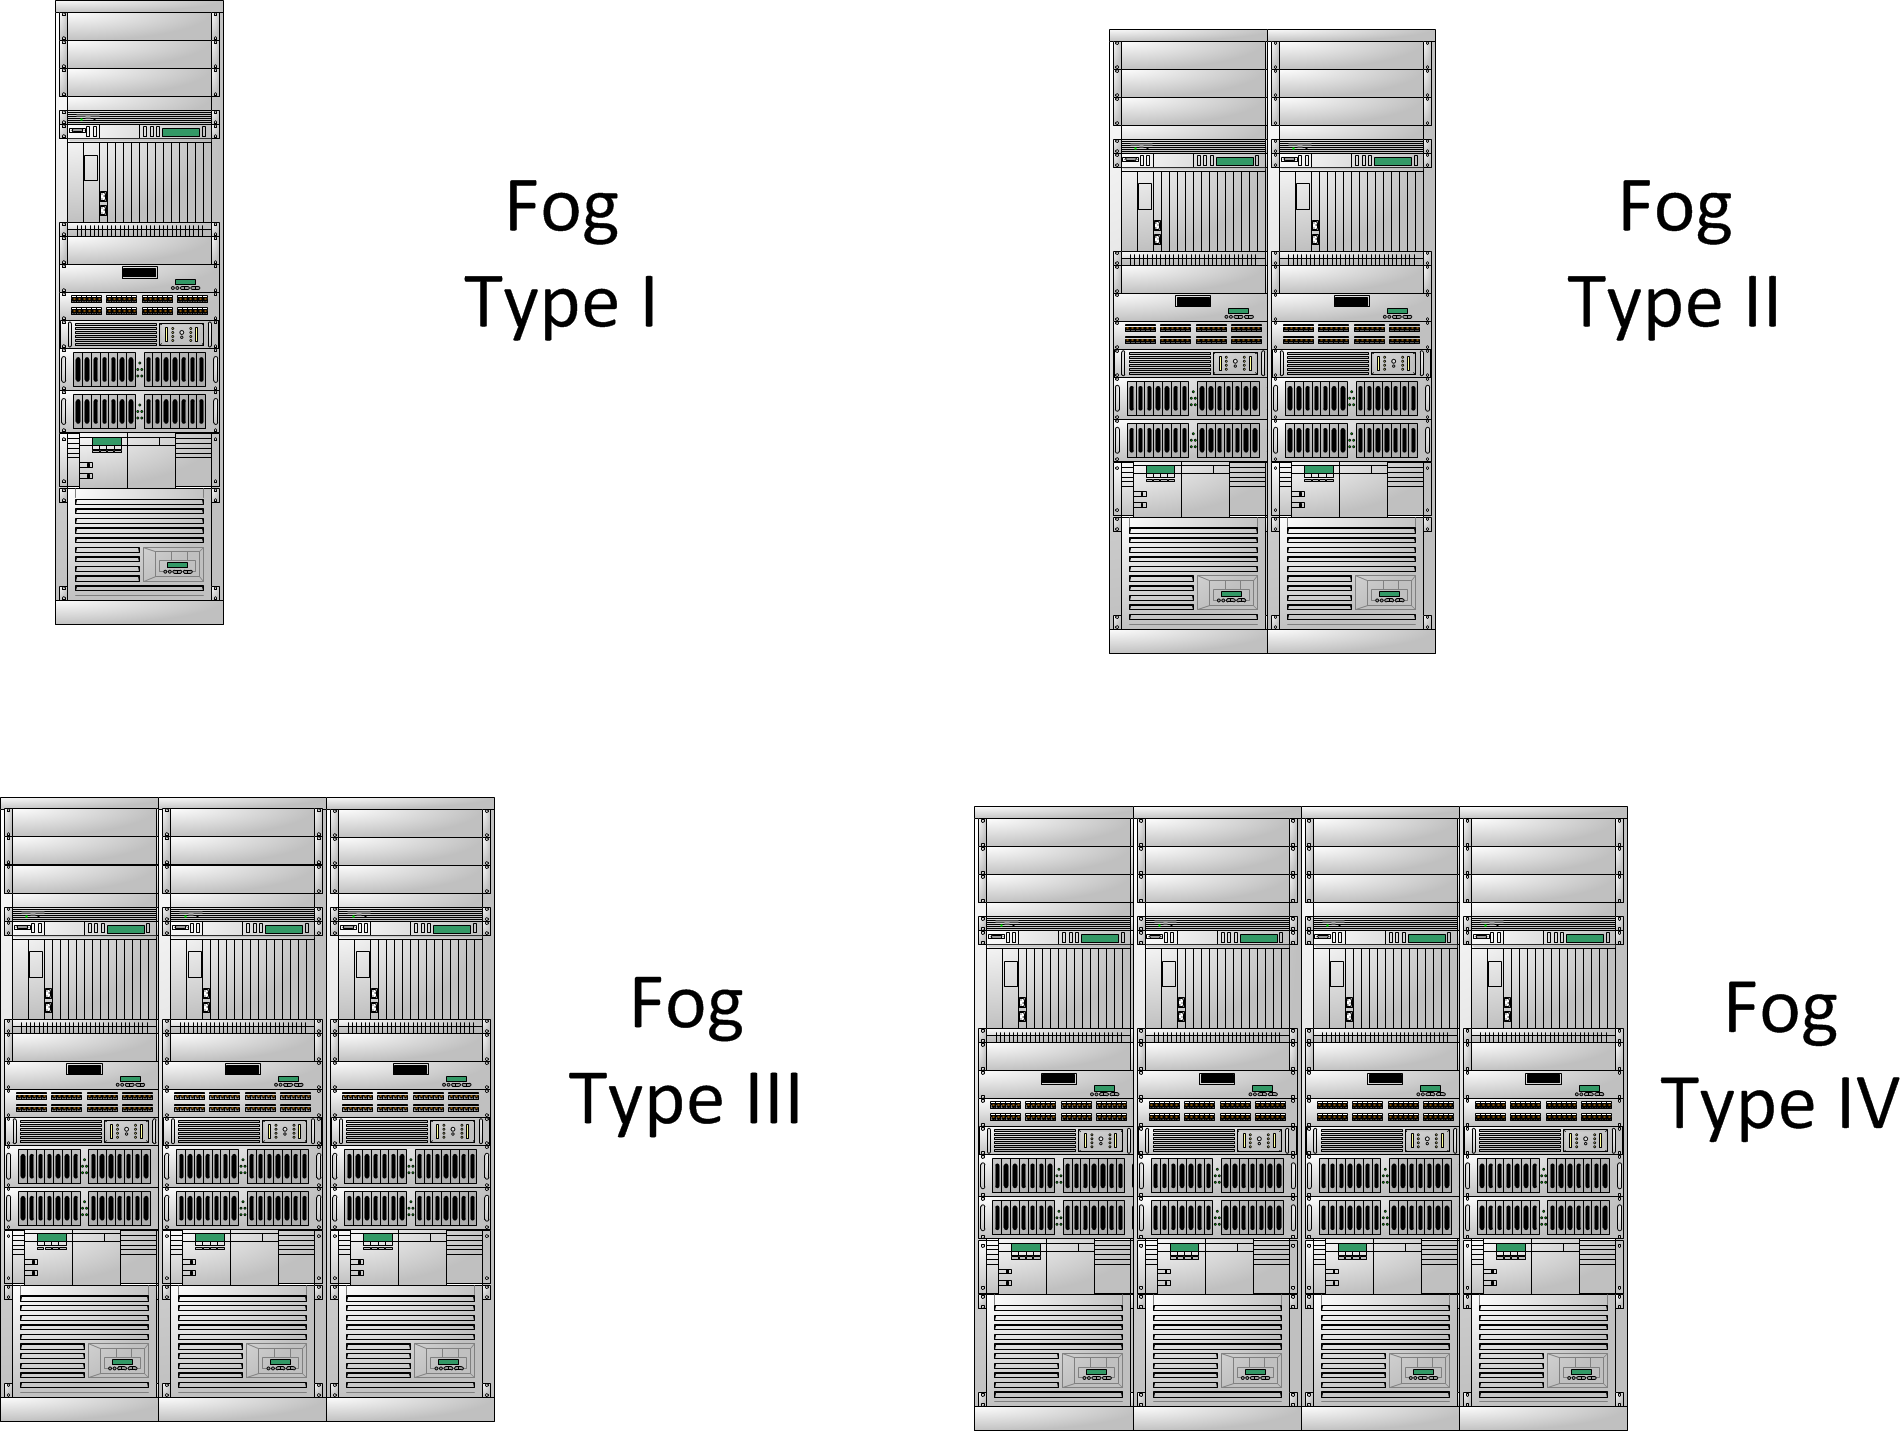
\includegraphics[width=3.in]{Drawing1.png}}
\caption{Fog Type} 
\label{rack}
\end{figure}
\fi
And their capacities and costs are described as Table \ref{fogprofiles1}.
\begin{table}[H]
\caption{Fog Profiles}
\label{fogprofiles1}

\resizebox{0.9\linewidth}{!}{%
\begin{tabular}{ | r| r | r | r | r | }
\hline
	Fog Type  & \# of CPU & Memory(MB) & NIC(Mbps) & Cost(USD) \\ \hline
	1 & 90 & 480 & 360 & 67200 \\ \hline
	2 & 180 & 800 & 1024 & 120000 \\ \hline
	3 & 360 & 1600 & 1024 & 170000 \\ \hline
	4 & 720 & 3200 & 10240 & 250000 \\ \hline
\end{tabular}}\\

\end{table}
\iffalse
\subsubsection{Point to Point delay as Network Usage}
Since the network usage function is transparent to optimization model, without loss generality, we use point to point delay to calculate network usage. In other words, our experiment try to find the trade-off Pareto front with regard to cost objective and delay objective.
$$
D(d_{ab})  = 
	\begin{cases}
	\begin{aligned}
	&\psi^{ToFog} + \mu^{ToFog} + \gamma^{ToFog} \\
	&\quad\quad(\sum_{i \in I  \setminus m}x_{ij} =1, \textit{(connect to fog)})\\
	
	&\psi^{ToCloud} + \mu^{ToCloud} + \gamma^{ToCloud} \\
	&  \quad\quad\quad  ( x_{mj} = 1, \textit{(connect to cloud)})
	\end{aligned}
	\end{cases}
$$


\subsubsection{Simulation Environment}
All the simulation runs on a HP workstation with Quad core processor, 2.66GHz internal clock and 4.00GB memory. The MIP optimizer CPLEX 12.07 was used in Weighted Sum Method, and the obtained results were used to evaluate the quality of NSGAII, SMPSO, PSONSGA heuristic algorithm. The input files, problem formation were modeled in JAVA language. NSGAII, SMPSO source code due to JMETAL framework\cite{Durillo2011} . PSONSGA was also implement in JAVA language.

\subsection{Weighted Sum Method on FPP with CPLEX}
We first apply the weighted sum method to solve the problem. To produce the Pareto front of each \# - \#problem instance, we use 11 pairs of weights to generate the weighted single objective functions. Solving each of these single objective functions by CPLEX can hopefully gives our N points Pareto front solution \Fig{espf}. ($N < 11$, because different weight pairs may converge to same point).
For each weight pair running, the CPLEX solver time limit was set to 2h. And the total running for single Pareto front solve time limit equals to (2 x 11)h. 
\fi
\iffalse
\begin{table}[H]
\caption{Weights Table}
\label{weightpair}
\centering
\begin{tabular}{ | l | l | l | l | }
\hline
	0 & 1 & $\Longrightarrow$ & 0 *OBJ1+1 *OBJ2 \\ \hline
	0.1 & 0.9 & $\Longrightarrow$ & 0.1 *OB+0.9 *OBJ2 \\ \hline
	0.2 & 0.8 & $\Longrightarrow$ & 0.2 *OBJ1+0.8 *OBJ2 \\ \hline
	0.3 & 0.7 & $\Longrightarrow$ & 0.3 *OBJ1+0.7 *OBJ2 \\ \hline
	0.4 & 0.6 & $\Longrightarrow$ & 0.4 *OBJ1+0.6 *OBJ2 \\ \hline
	0.5 & 0.5 & $\Longrightarrow$ & 0.5 *OBJ1+0.5 *OBJ2 \\ \hline
	0.6 & 0.4 & $\Longrightarrow$ & 0.6 *OBJ1+0.4 *OBJ2 \\ \hline
	0.7 & 0.3 & $\Longrightarrow$ & 0.7 *OBJ1+0.3 *OBJ2 \\ \hline
	0.8 & 0.2 & $\Longrightarrow$ & 0.8 *OBJ1+0.2 *OBJ2 \\ \hline
	0.9 & 0.1& $\Longrightarrow$ & 0.9 *OBJ1+0.1 *OBJ2 \\ \hline
	1 & 0 & $\Longrightarrow$ & 1 *OBJ1+0 *OBJ2 \\ \hline
\end{tabular}
\end{table}

\begin{figure}[H]
\centerline{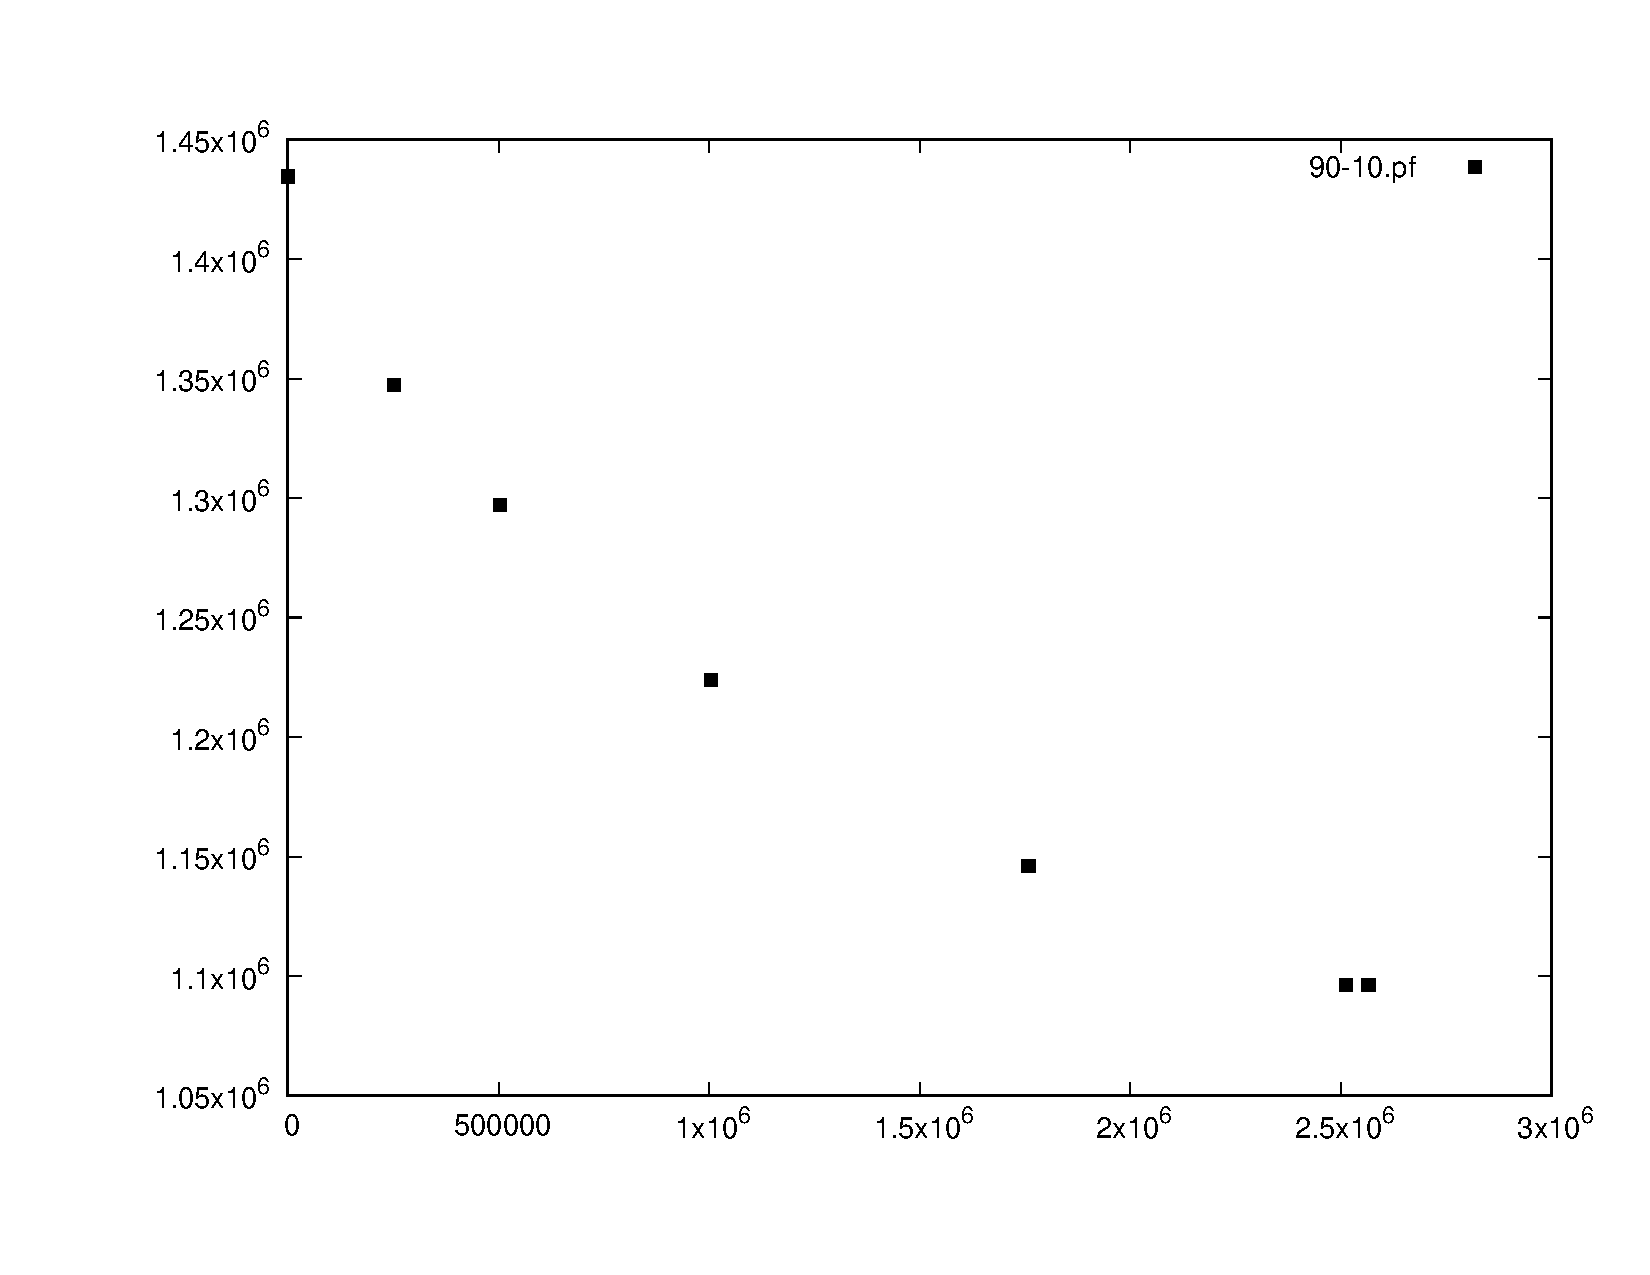
\includegraphics[width=3.5in]{9010pf.pdf}}
\caption{Exact Solution Pareto Front} 
\label{espf}
\end{figure}
Since each "InstanceBundle" has different size of FPP problems. Executing same procedure upon different problems give us a general picture of the computation efficiency and solution quality of weighted sum method.
As can be seen in \Fig{cplex-compu}, the computation time increased exponentially as the problem size increased. 
For a 90-10 problem (90 users, 10 potential location), it will take 7.061 hour ( 25421955 ms) to give out a 10\% gap  solution. 

%\begin{figure*}[!t]
%\centering
%\subfloat[Case I]{\includegraphics[width=2.5in]{box}%
%\label{fig_first_case}}
%\hfil
%\subfloat[Case II]{\includegraphics[width=2.5in]{box}%
%\label{fig_second_case}}
%\caption{Simulation results for the network.}
%\label{fig_sim}
%\end{figure*}
\begin{figure*}[!t]
\centering
\subfloat[CPLEX Pareto Front]{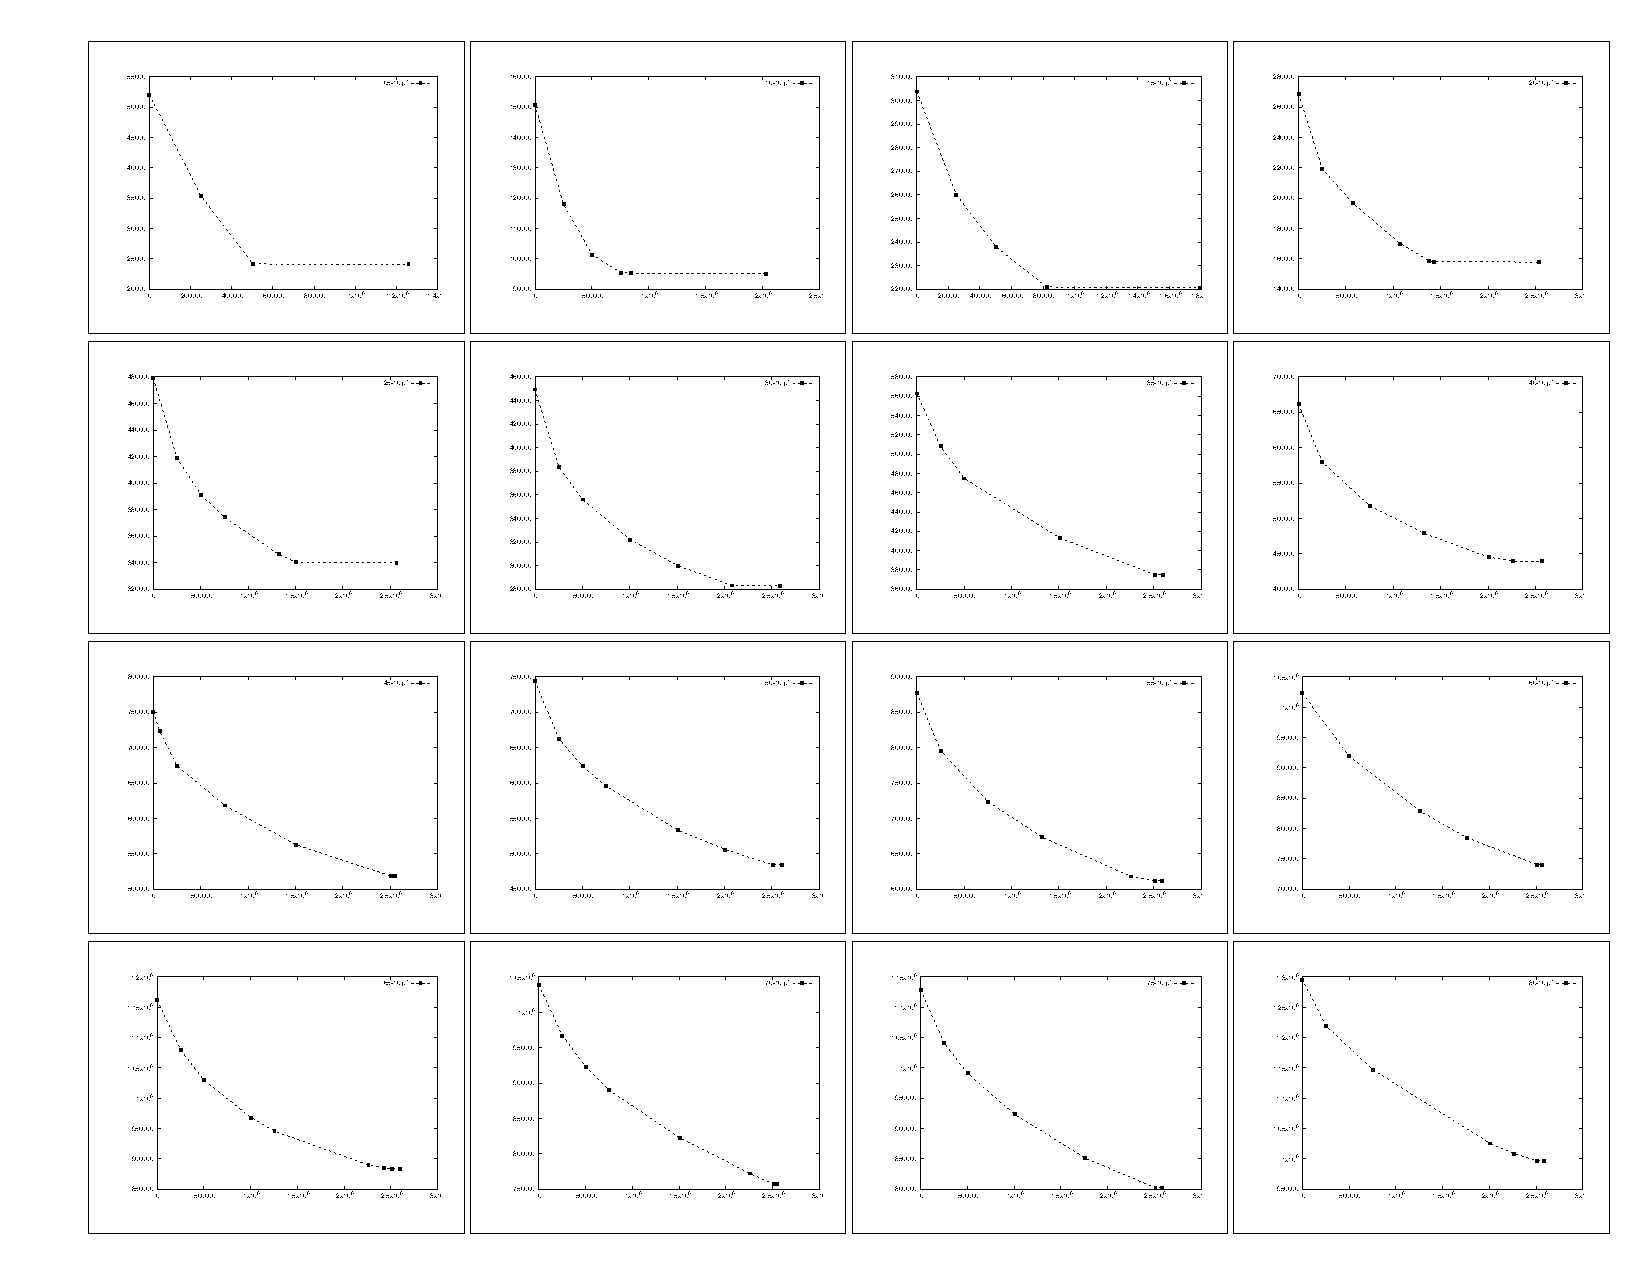
\includegraphics[width=3.5in]{cplexTotal.pdf}%
\label{cplexTo}}
\hfil
\subfloat[CPLEX Execution Time and Computation Gap]{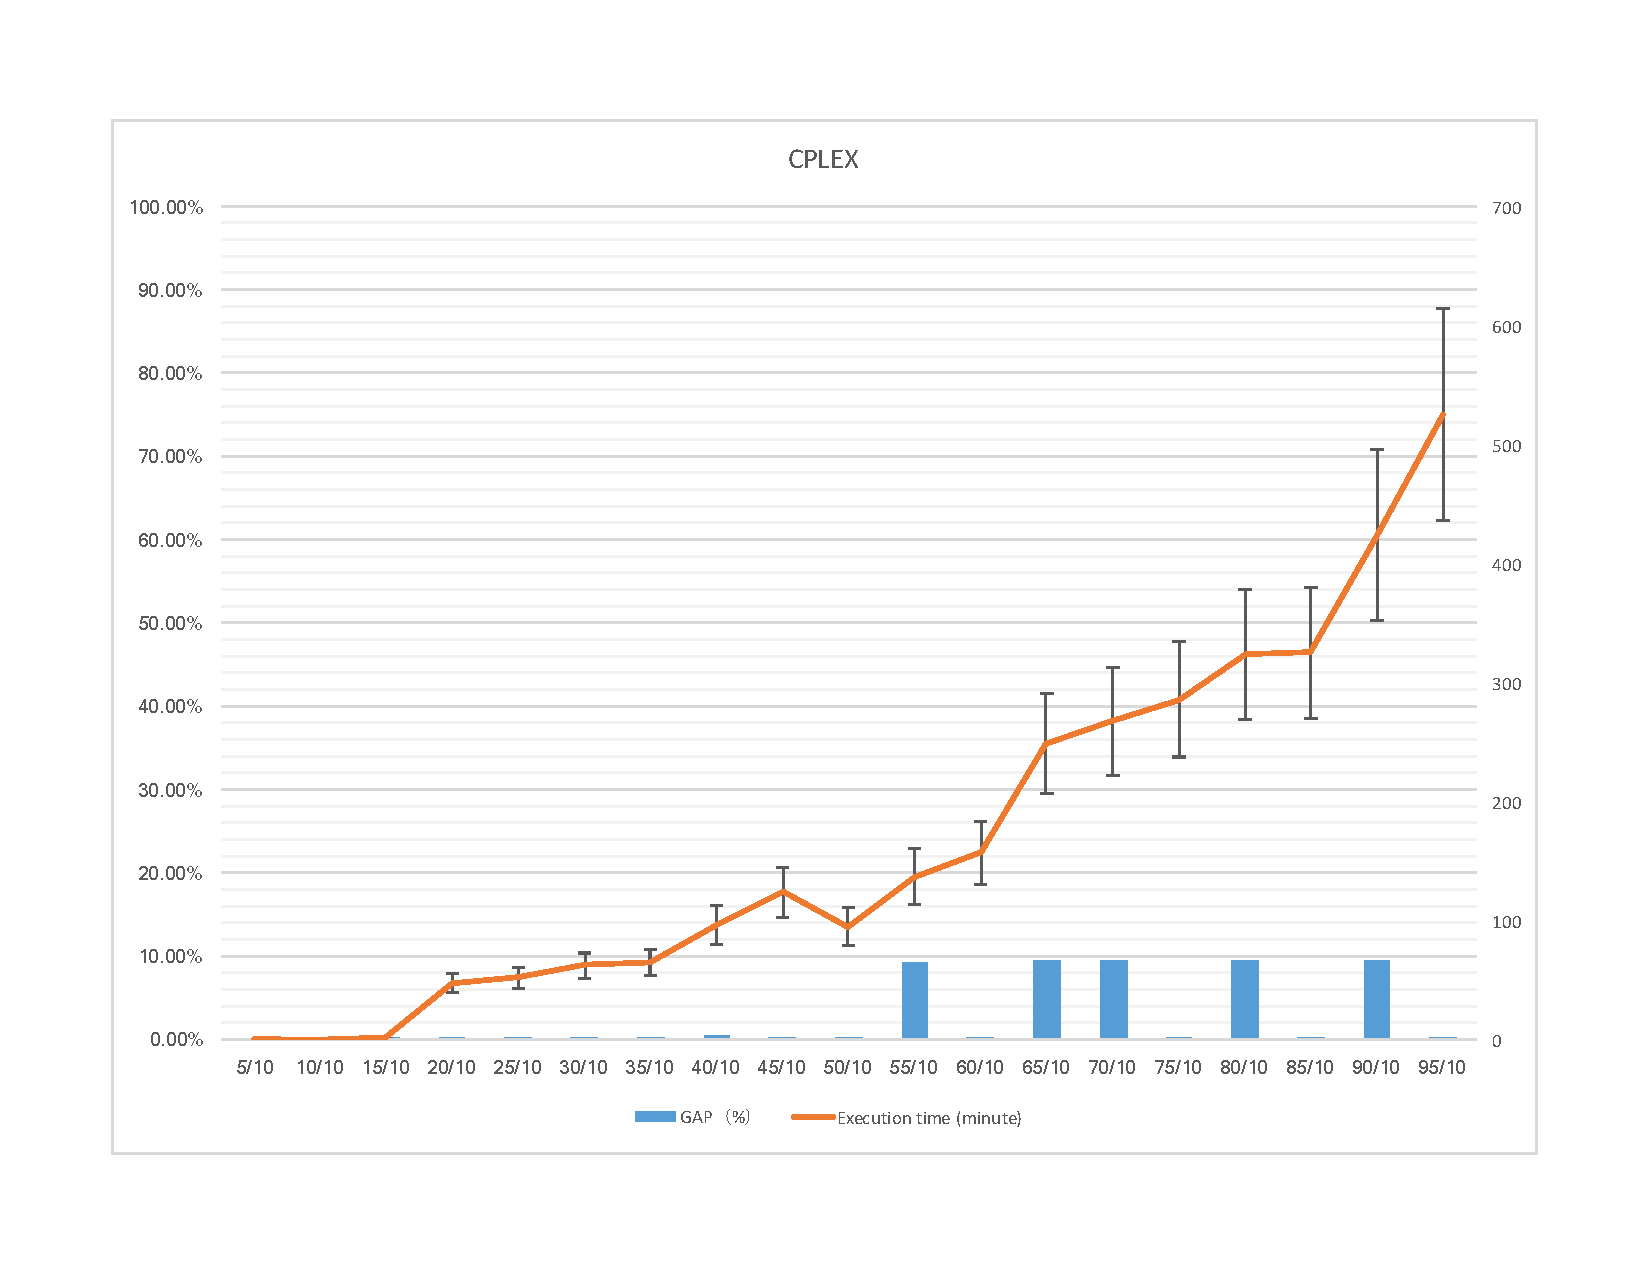
\includegraphics[width=3.5in]{cplex-computation-time.pdf}%
\label{cplex-compu}}
\caption{CPLEX Result} 
\label{cplex-compose}
\end{figure*}
Noticeably, even if we run 11 single-objective optimizations. We cannot expect to get 11 point solutions (11 different non-dominated solution forming Pareto Front). Because, two different weight settings may converge to same planning result; therefore, gives same objective function values. And we can not know they will give same result before CPLEX execution finished. Also, to produce a Pareto front with higher granularity, the only option is to increase the weight pair number. For small size problem, this may be a valid approach. Whereas, for big size problem, for example 90-10 FPP, the long computation time of MIP solver makes this approach less effective.
\fi
\subsection{Detailed Example}
In this section, a detailed example is presented to explain the FPP planning results. The first instance of FPP3010 is solved with the weighted sum method, NSGA-II, SMPSO and PSONSGA algorithms. The FPP3010 assumes that one needs to plan and design a brand new fog network to accommodate 30 edge-clusters. To achieve this, we need to find the optimal number, location and capacity of fog nodes. \Fig{nettopology} shows the initial planning area with 30 edge-clusters and 10 potential locations that are uniformly distributed in a $100km \times 100km$ area. 
Each edge-cluster has resource demands which need to be accommodated. 
\begin{figure}[H]
\centerline{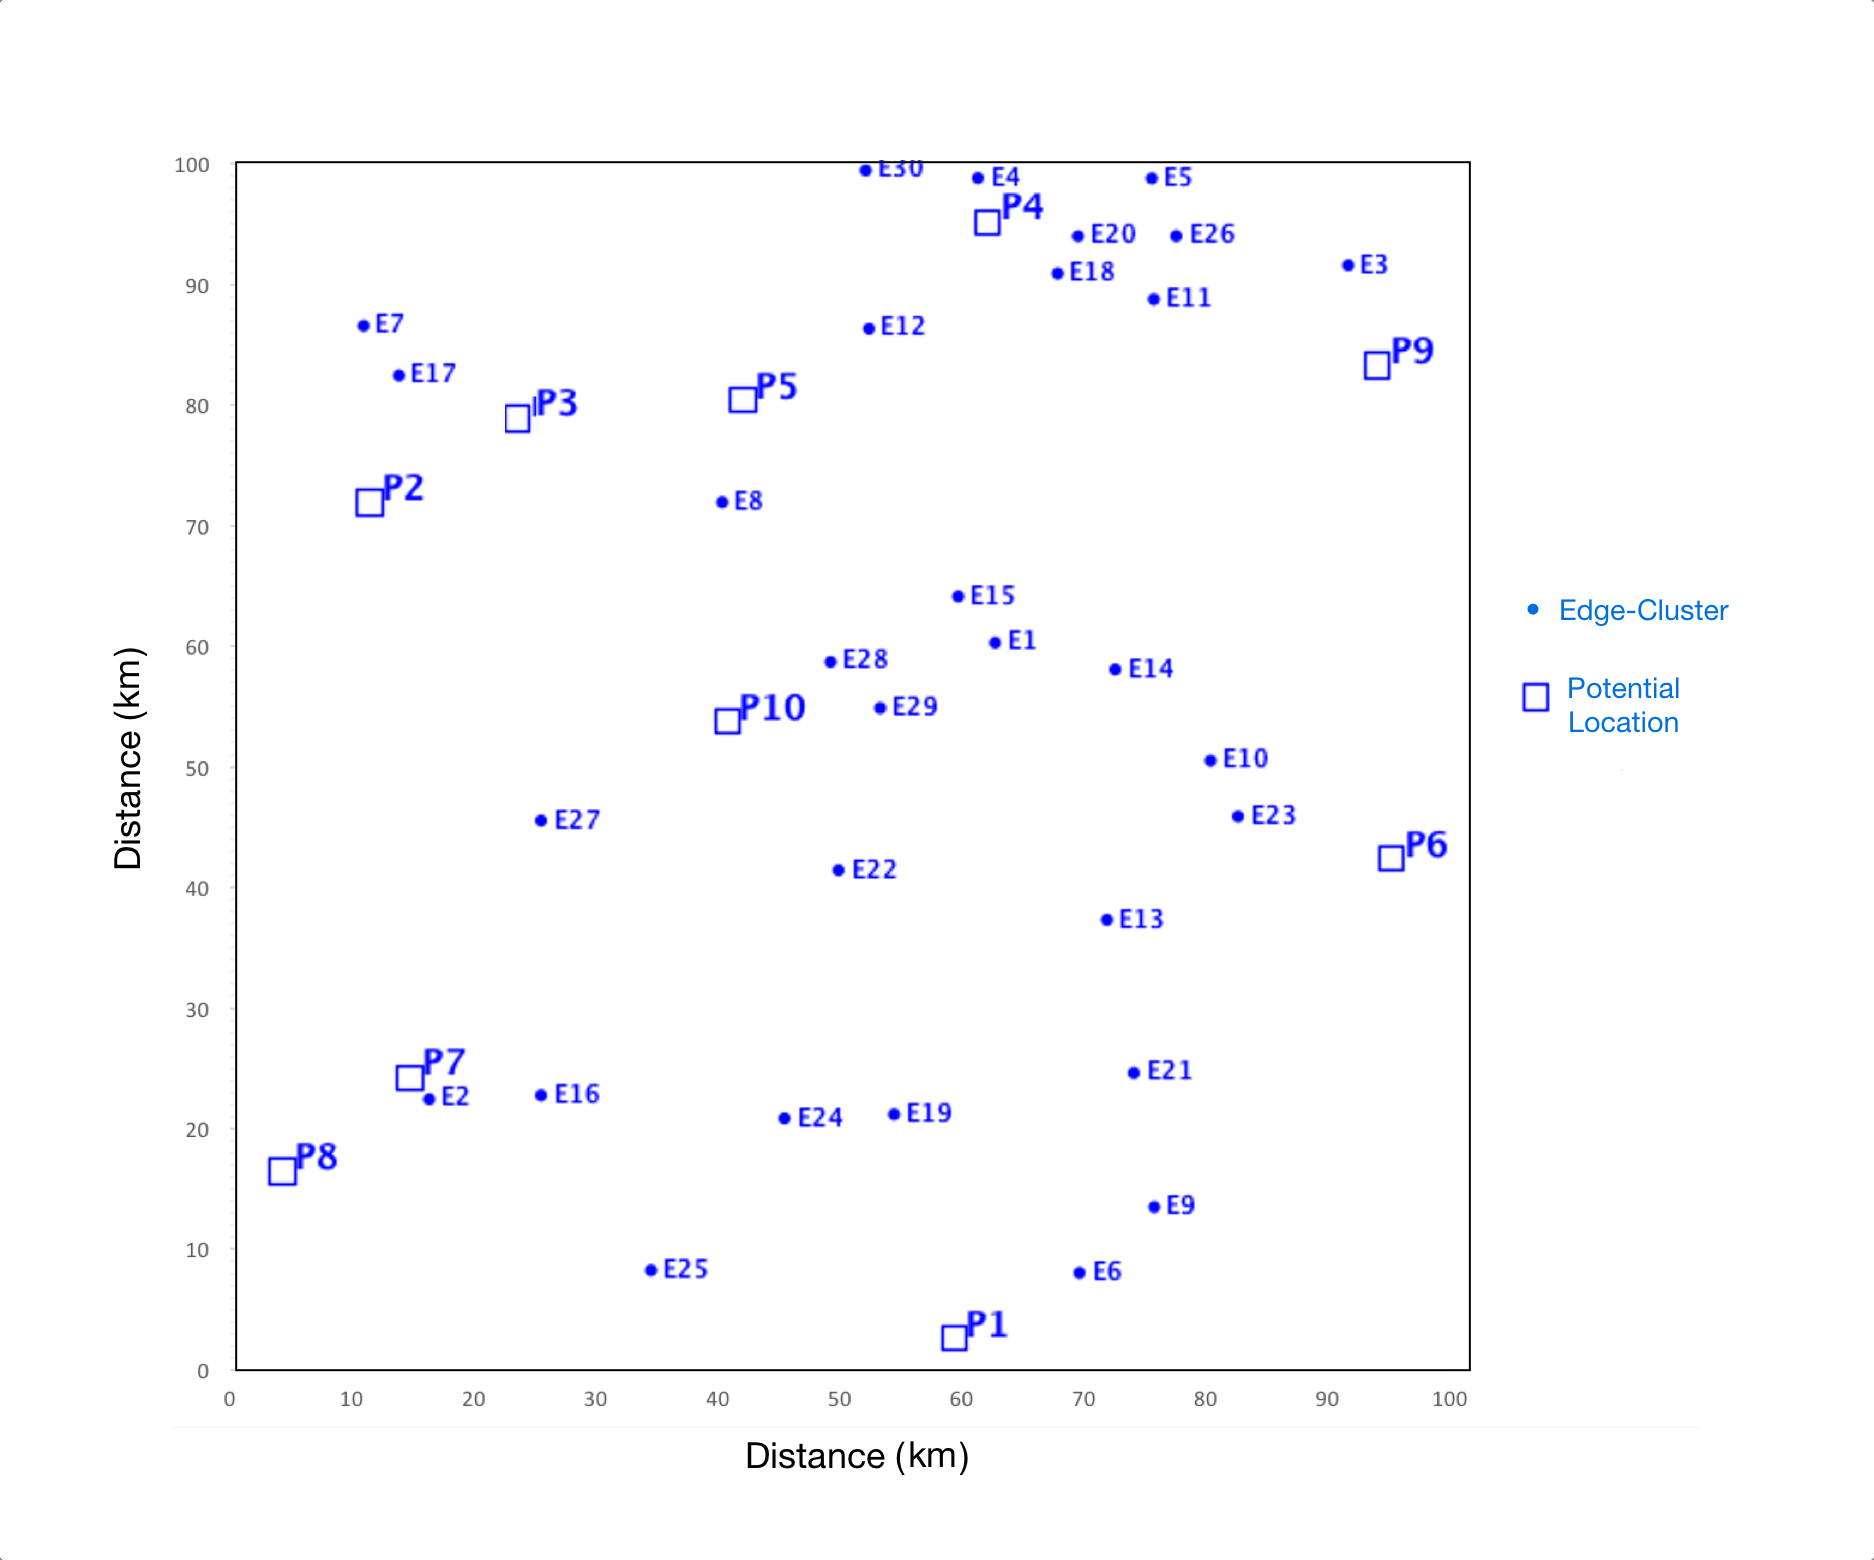
\includegraphics[trim=0 50 0 50,clip,width=3.8in]{100x100problem.png}}
\caption{Edge-cluster locations and potential locations of fog for FPP3010 (instance-1)} 
\label{nettopology}
\end{figure}
\subsubsection{Results from the Weighted Sum Method}
The results for problem FPP3010 (instance-1) by using the weighted sum method are shown in Table \ref{CPLEXresultssample}. The first column shows the solution index which makes reference to the 11 different weight combinations. The following two columns contain the decision output for the link type and the fog type at each location. Columns 4 and 5 provide the results of the two objective functions (cost and delay respectively) obtained with the weighted sum method. Finally, column 6 shows the relative Mixed-Integer Programming (MIP) gap. The MIP gap represents the percentage gap between the solution value found by CPLEX and the value of the optimal. For example, a 0.05 relative MIP gap means that CPLEX has found a solution that is five percent from the optimal. Using CPLEX to solve the FPP3010 (instance-1), we can find 7 solution frontiers (as shown by the 7 different solutions from Table \ref{CPLEXresultssample}, the duplicated results are grey colored) . 


\begin{table}
\centering
\caption{CPLEX's result for problem FPP3010}
\label{CPLEXresultssample}

\resizebox{\columnwidth}{!}{
\begin{tabular}{|c|c|c|c|c|c|}
\hline
\textbf{Solution} &\textbf{Link output}&\textbf{Fog output}&\textbf{Cost }&\textbf{Delay}  &\textbf{Gap}\\
\textbf{number} &&&\textbf{(\$)}&\textbf{(ms)}& \textbf{(\%)}\\

\hline
\hline
1&1 1 1 1 1 1 1 1 1 1	&4 1 4 3 4 4 4 4 4 4	&2586500.0&283&0.0\\
2&1 1 1 1 1 1 1 0 1 1	&4 1 4 4 4 4 4 0 4 4	& \cellcolor{gray25}2078225.0& \cellcolor{gray25}283&9.94e-5\\
3&1 1 1 1 1 1 1 0 1 1	&4 1 4 4 4 4 4 0 4 4	& \cellcolor{gray25}2078225.0& \cellcolor{gray25}283&9.98e-5\\
4 &1 1 1 1 1 1 1 0 1 1	&4 1 4 4 4 4 4 0 4 4	&\cellcolor{gray25}2078225.0& \cellcolor{gray25}283&9.99e-5\\
5&0 0 1 1 1 0 1 0 1 1	&0 0 4 4 4 0 4 0 4 4	&1507350.0&300&0.0047\\
6&0 0 1 1 1 0 0 0 0 1	&0 0 4 4 4 0 0 0 0 4	&1004900.0&322&9.80e-5\\
7&0 0 1 0 0 0 0 0 0 1	&0 0 4 0 0 0 0 0 0 4	&502450.0&356&7.69e-5\\
8& 0 0 1 0 0 0 0 0 0 0	&0 0 4 0 0 0 0 0 0 0	&\cellcolor{gray25}251225.0& \cellcolor{gray25}384&0.0\\
9& 0 0 1 0 0 0 0 0 0 0	&0 0 4 0 0 0 0 0 0 0	&\cellcolor{gray25}251225.0& \cellcolor{gray25}384&0.0\\
10&0 0 0 0 0 0 0 0 0 0	&0 0 0 0 0 0 0 0 0 0	& \cellcolor{gray25}0.0& \cellcolor{gray25}449&0.0\\
11&0 0 0 0 0 0 0 0 0 0	&0 0 0 0 0 0 0 0 0 0	& \cellcolor{gray25}0.0& \cellcolor{gray25}449&0.0\\
\hline
\end{tabular}}
\end{table}
%\Fig{espf} shows the Pareto front in Table \ref{CPLEXresultssample}. 
\iffalse
\begin{figure}[H]
\centerline{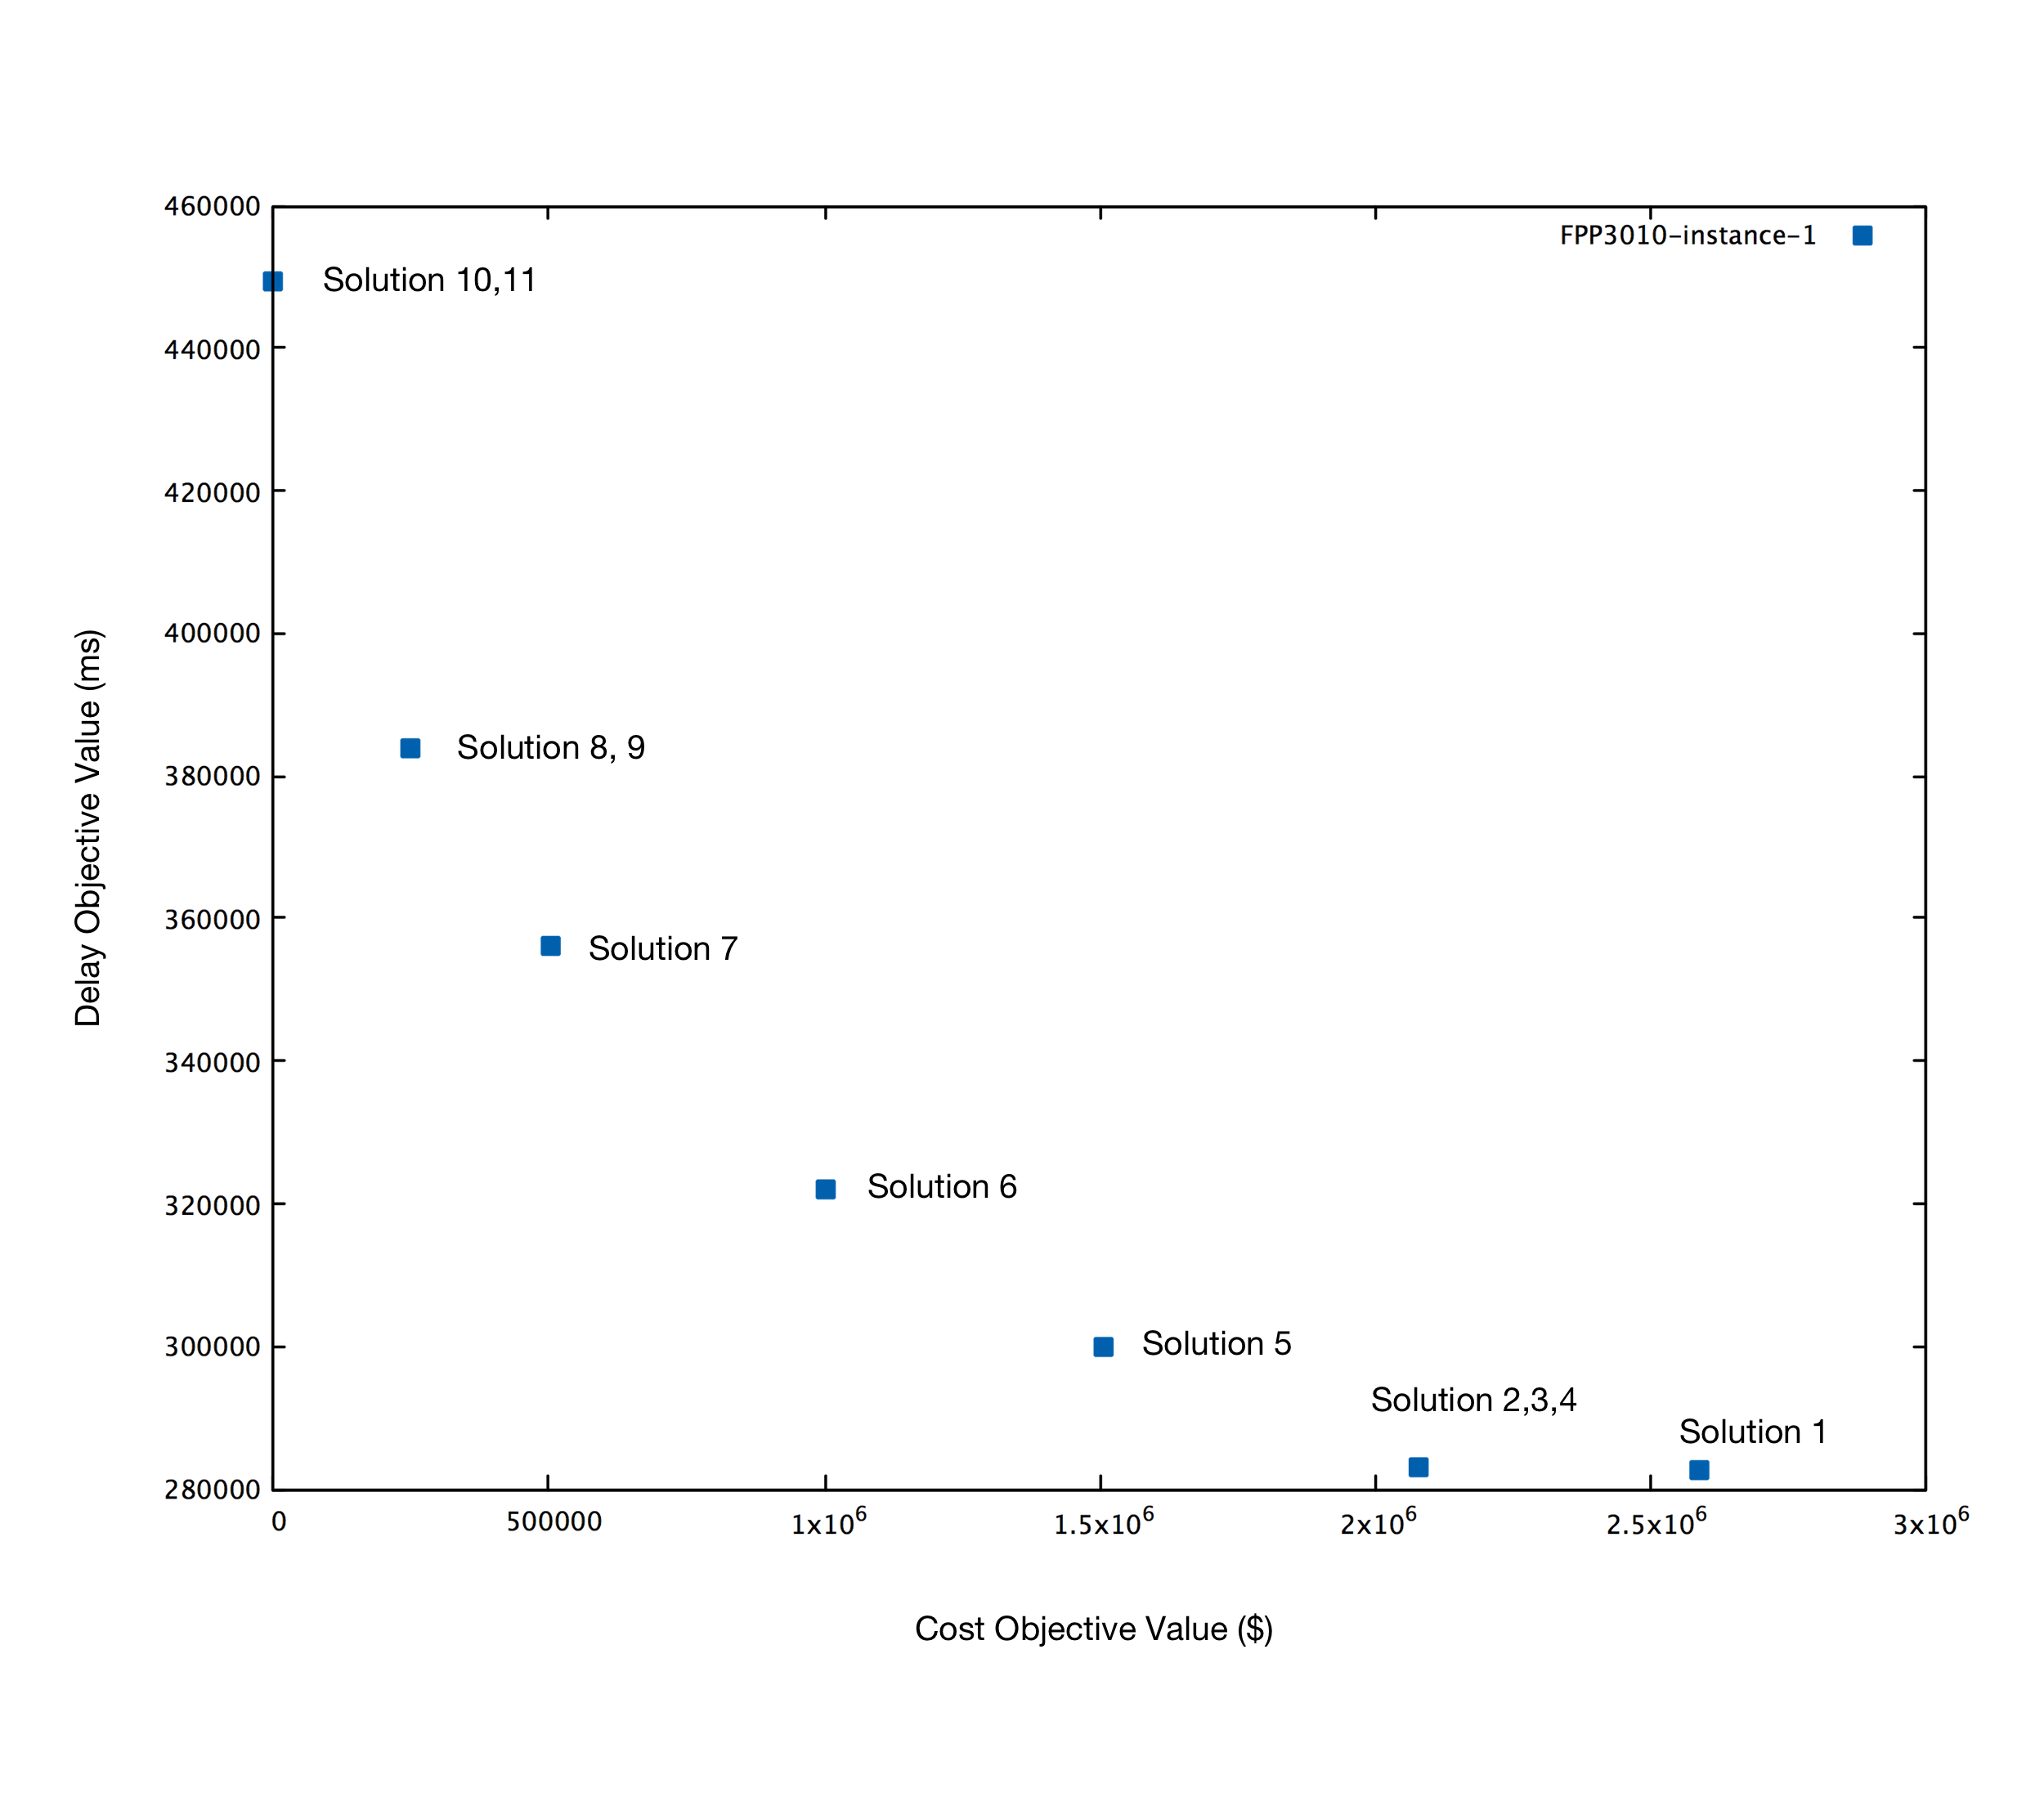
\includegraphics[width=5.5in]{FPP3010-instance1png.png}}
\caption{An example of exact solution Pareto front} 
\label{espf}
\end{figure}
\fi

Noticeably, %even if we run 11 single-objective optimizations. We cannot expect to get 11 point solutions (11 different non-dominated solutions). Because,
different weight settings may converge to the same objective function values (for example, see solutions 2, 3, 4 from Table \ref{CPLEXresultssample}). \Fig{CPLEXfro} plots the solution frontier obtained from the weighted sum method. 
\subsubsection{Results from Evolutionary Algorithms }
One fundamental difference between single and multiple objective optimization is the number of the solutions. Since several solutions can be optimal, each of these solutions represent a planning and routing scheme which considers a different cost/performance balance. An example of the 49 planning results (Pareto front) obtained with NSGA-II is presented in Table~\ref{table:solution.obj.nsgaii}. 
 %And we can not know they will give same result before CPLEX execution finished. Also, 
%To produce a Pareto front with higher granularity, we can increase the number of weight settings. For small-scale problems, this may be a valid approach. Whereas, for large-scale problems, CPLEX's CPU time is increasing exponentially with respect to the problem size. 
%Using CPLEX to solve the large-scale problems will be time-consuming. %The average computing time with 95\% confidence interval for different size of FPP is plotted in \Fig{CPLEX-compu}. As can be seen in \Fig{CPLEX-compu}, the computation time increases exponentially as the problem size increases.  For a 90-10 problem (90 users, 10 potential location), it takes approximately 7.061 hours (25421955 ms) to return a solution set. The relative MIP gaps also increases as the problem size scale up. It means that CPLEX cannot find the optimal solution within 1 hour for each weight setting, therefore, CPLEX returns the best solution found so far. Also, since the problem is NP-hard, even the memory of the computer may be insufficient. In this case, CPLEX returns the best solution found before it runs out of memory.
%As a result, the proposed evolutionary algorithm are more appropriate in this situation.

\begin{figure*}[!t]
 	\subfloat[Solution frontier of weighted sum (CPLEX)]
       {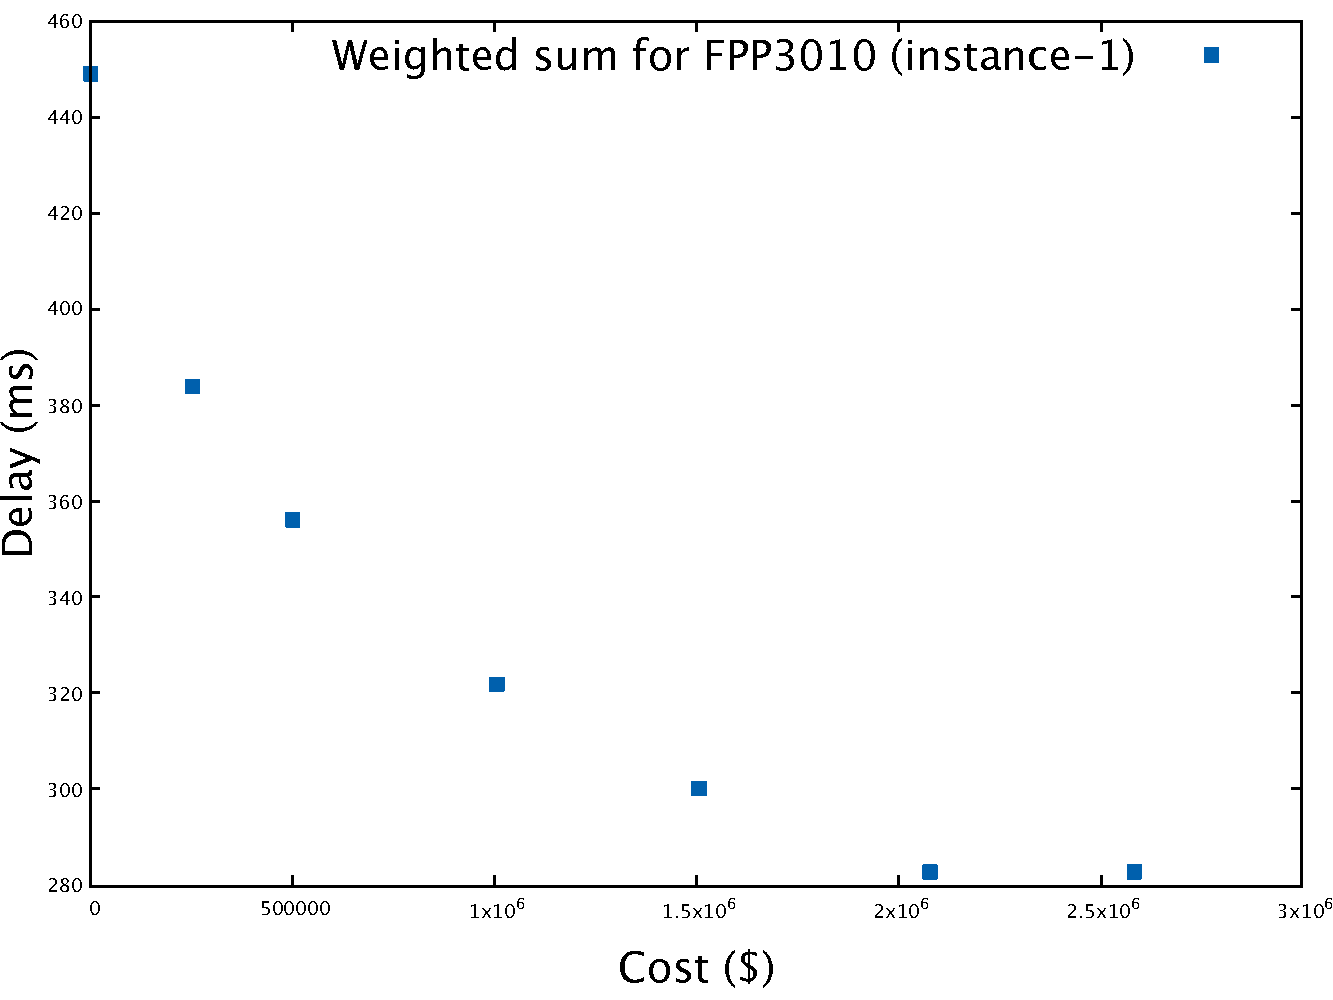
\includegraphics[trim=0 0 0 0,clip,width=0.5\linewidth]{ws_frontier.pdf}\label{CPLEXfro}} % first figure itself
       \hfil
        \subfloat[Solution frontier of NSGA-II]
        {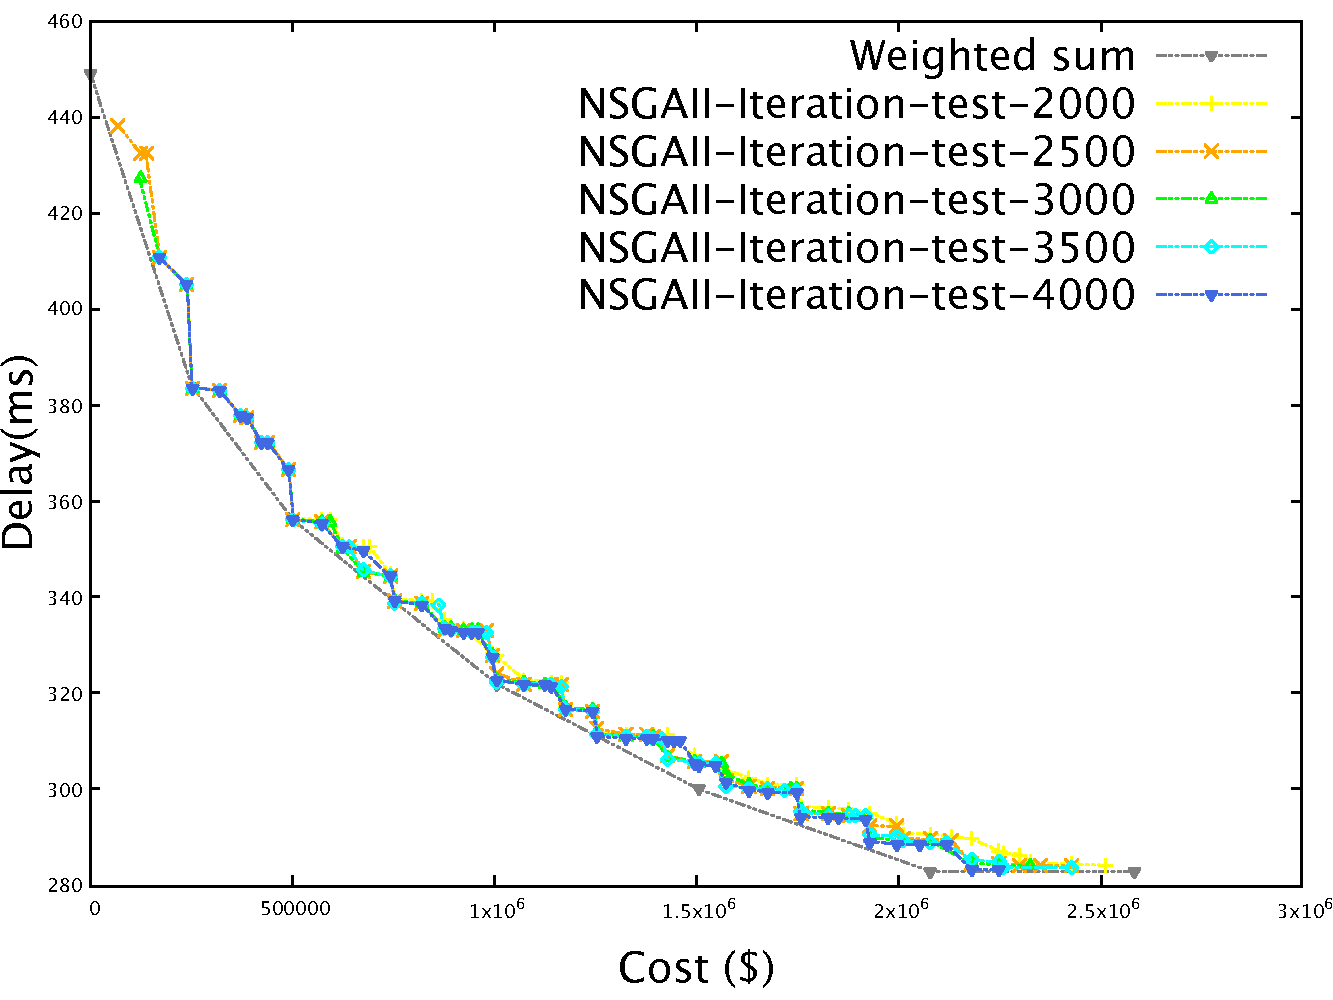
\includegraphics[trim =0 0 0 0,clip,width=0.5\linewidth]{nsga_frontier.pdf}\label{nsgafro}}% second figure itself
         %\captionsetup{font={scriptsize,}}
        
     % \vspace{10ex}

         
        % first figure itself
        % \captionsetup{font={scriptsize,}}
        \subfloat[Solution frontier of SMPSO]
        {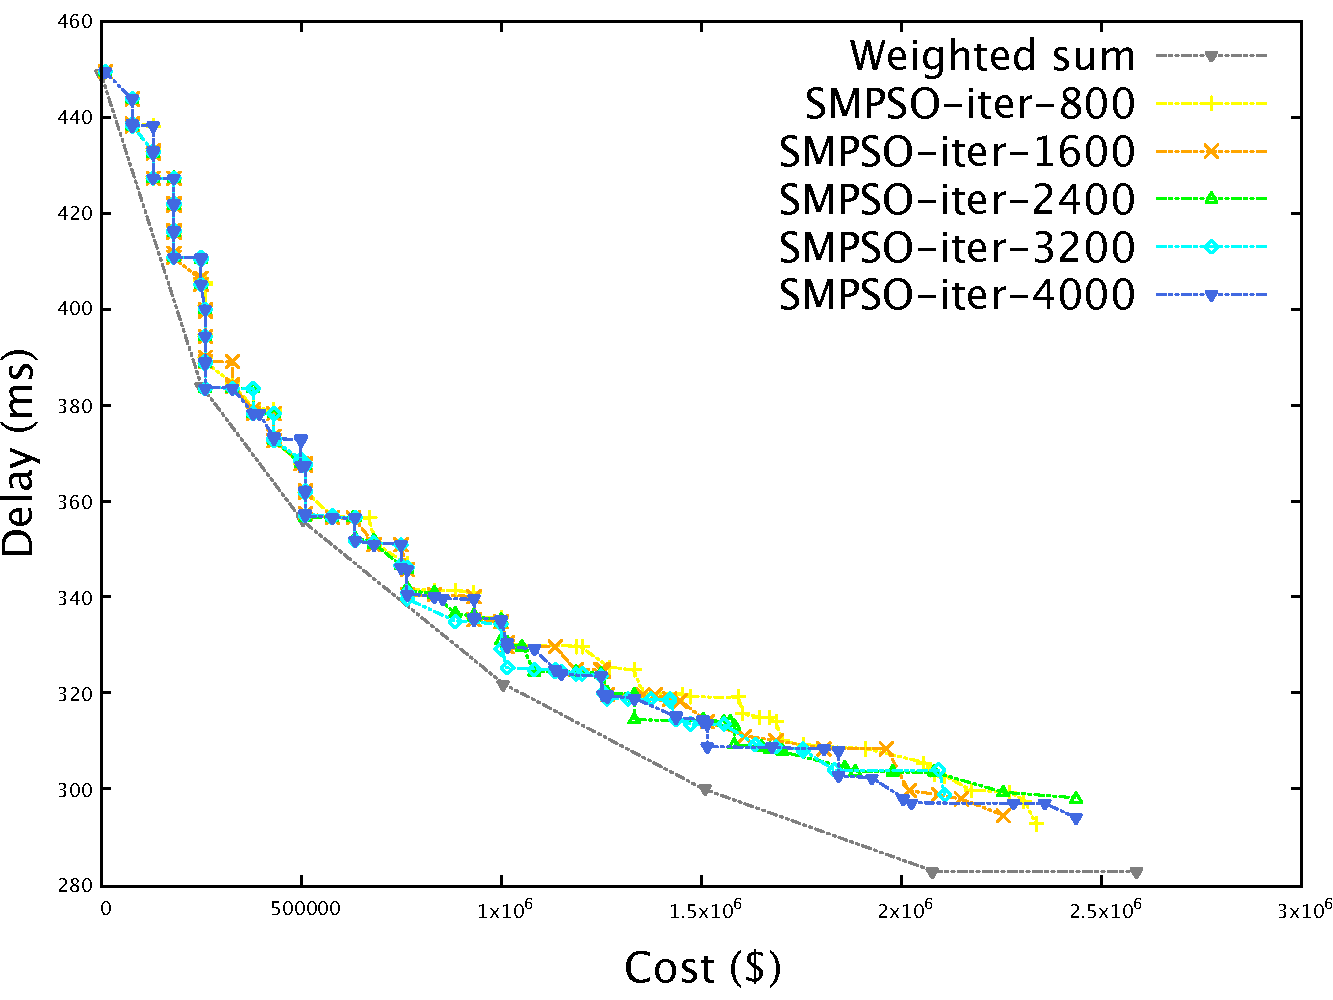
\includegraphics[trim=0 0 0 0,clip,width=0.5\linewidth]{smpso_frontier.pdf} \label{smpsofro}}
   \hfil
         % second figure itself
       % \captionsetup{font={scriptsize,}}
        \subfloat[Solution frontier of PSONSGA] 
        {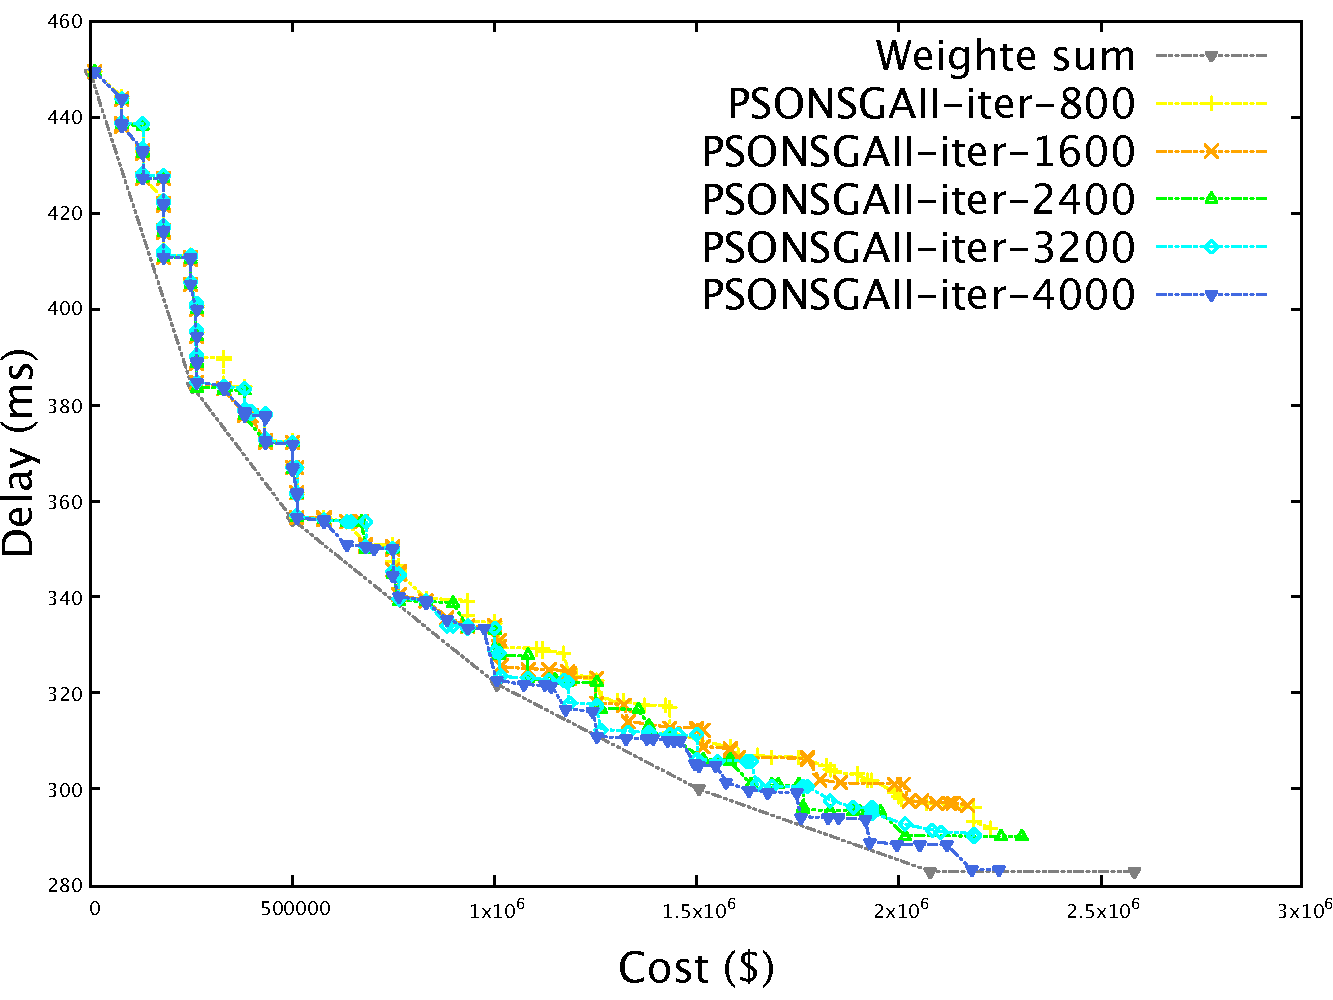
\includegraphics[trim=0 0 0 0,clip,width=0.5\linewidth]{psonsga_frontier.pdf}\label{psonsgafro}}
\caption{Solution frontier comparison}
\end{figure*}

\begin{figure*}[!t]
    
        % first figure itself
     %   \captionsetup{font={scriptsize,}}
        \subfloat[Planning result of weighted sum (CPLEX), cost: \$1,004,900 delay: 322.1ms]
        {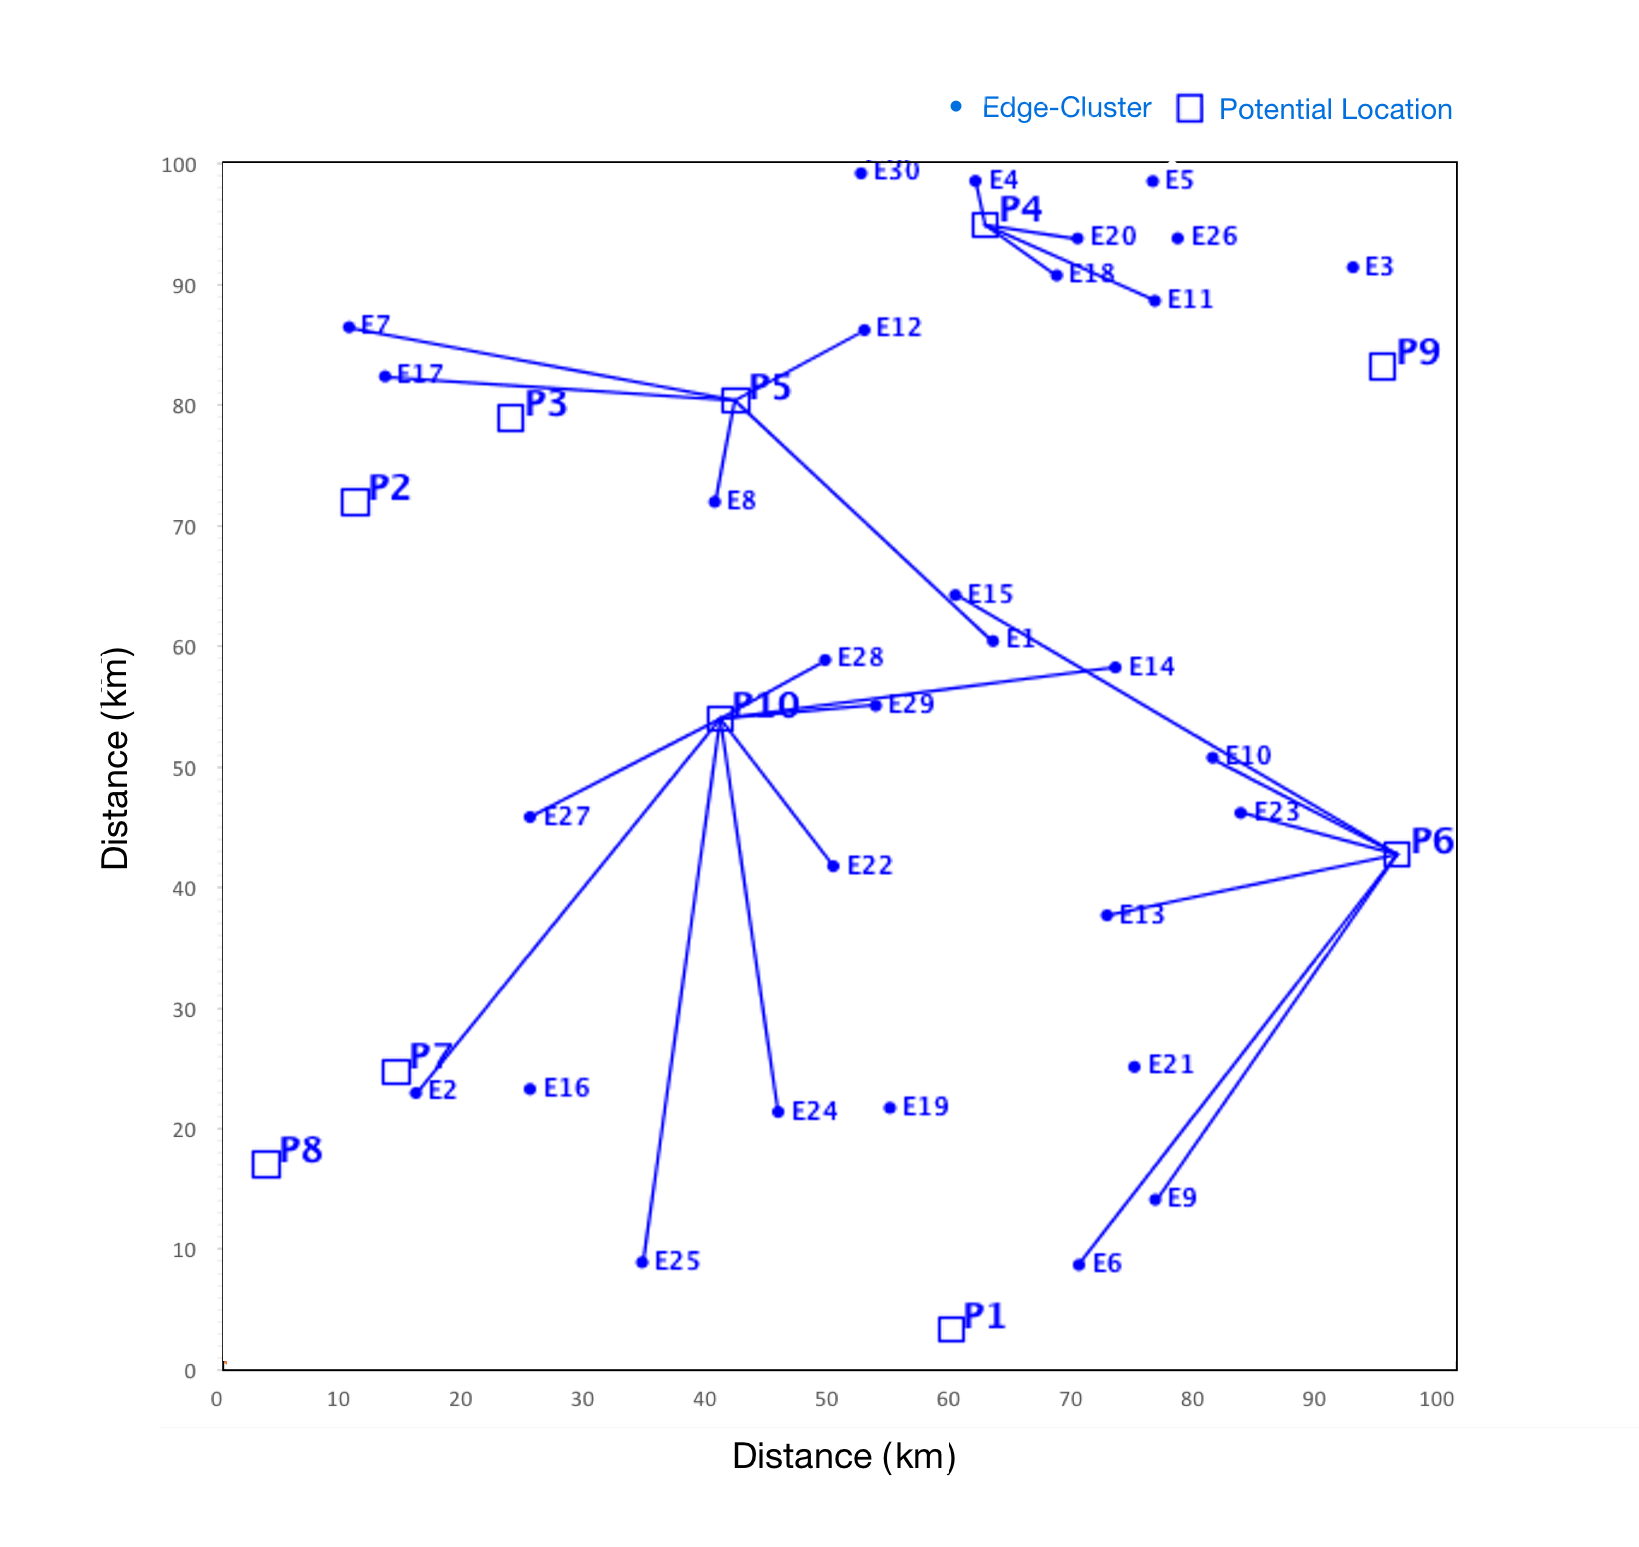
\includegraphics[trim=40 20 20 30,clip,width=.5\linewidth]{100x100problem_cplex2.png}\label{CPLEXrouting}}
    \hfil
        % second figure itself
       %  \captionsetup{font={scriptsize,}}
        \subfloat[Planning result of NSGA-II, cost: \$1,004,900 delay: 322.6ms]
        {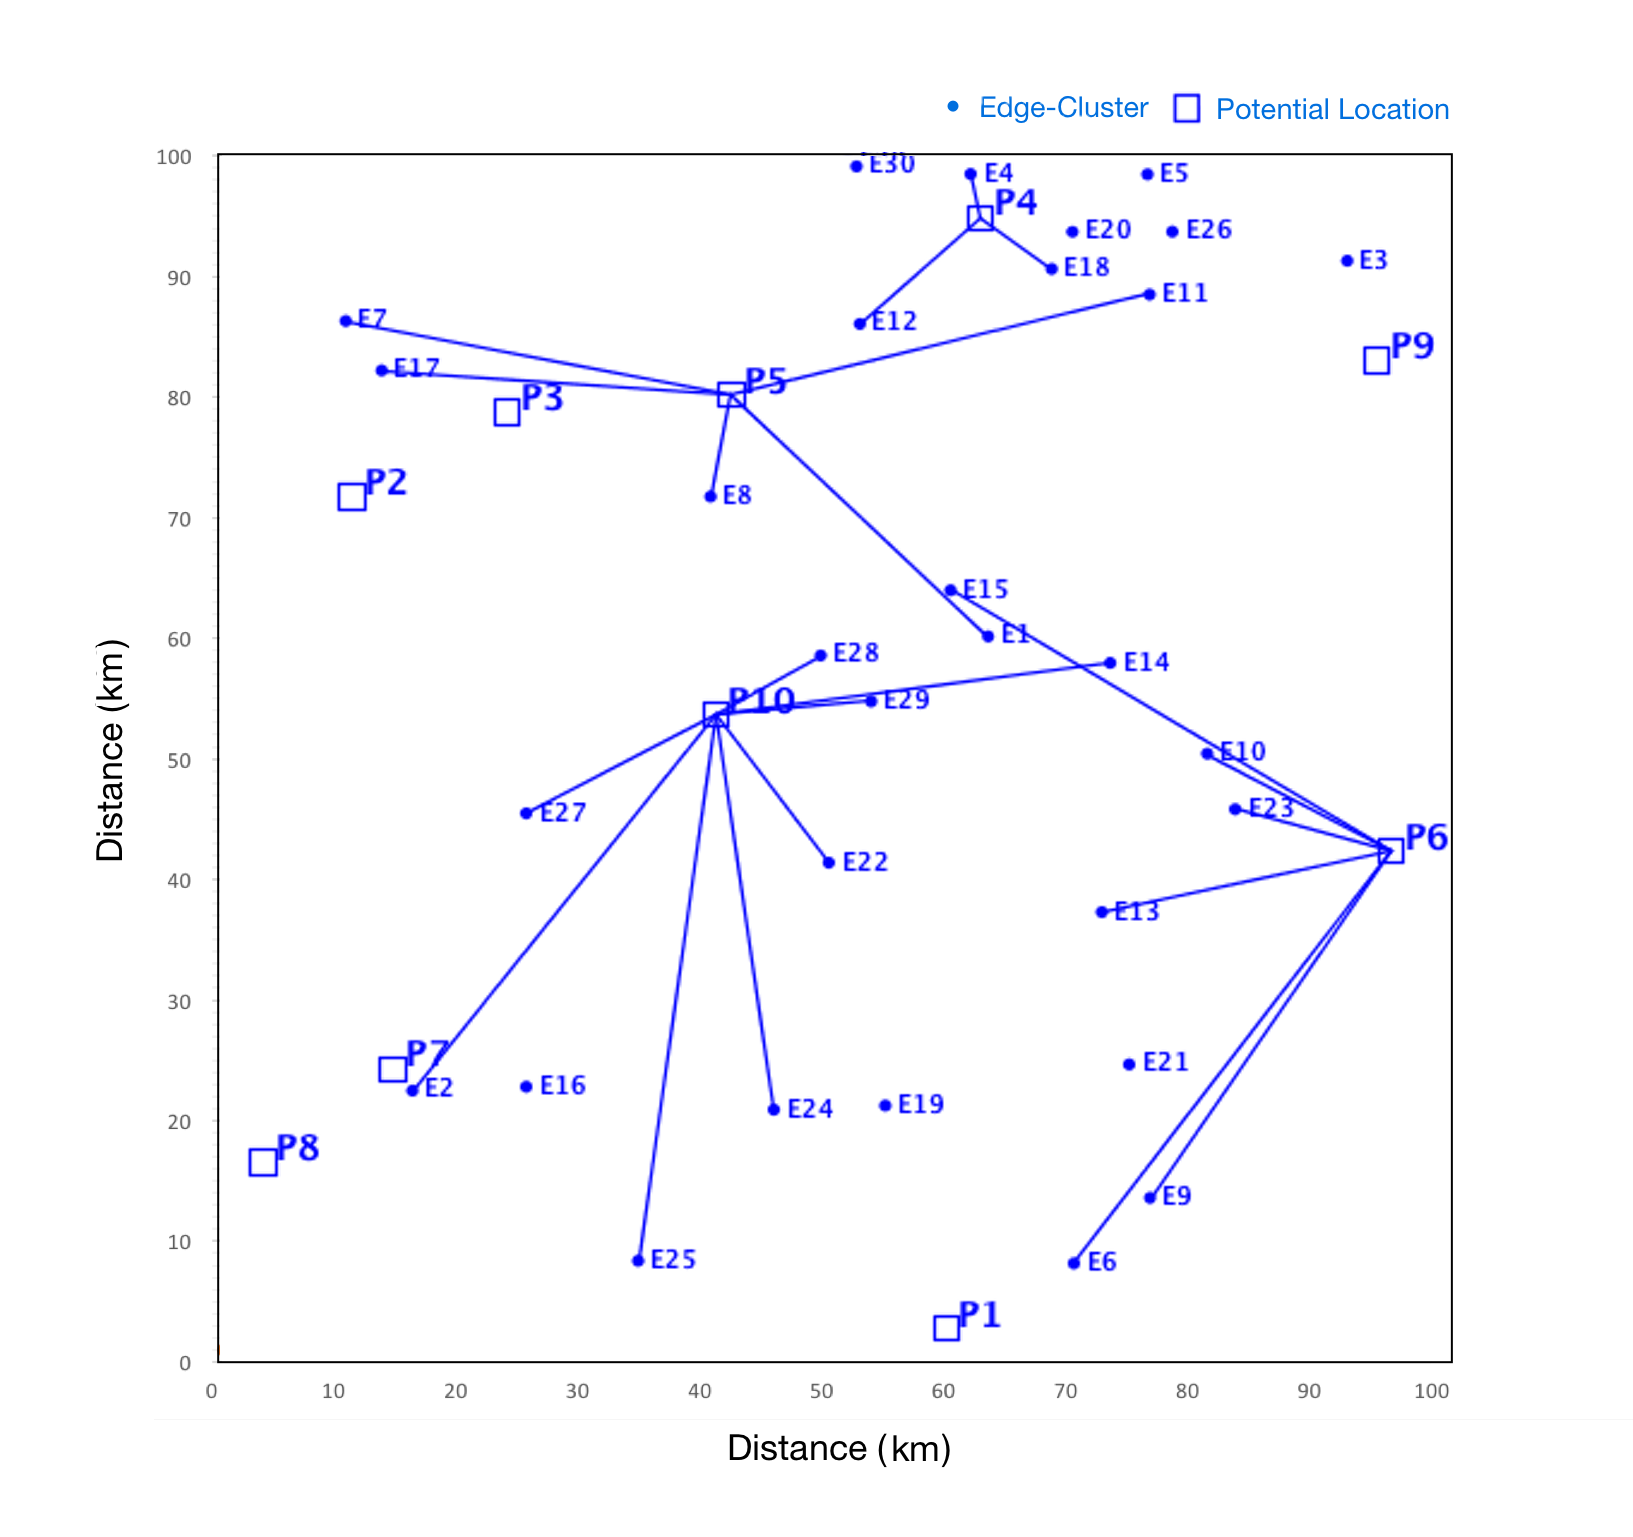
\includegraphics[trim =40 20 20 40,clip,width=0.5\linewidth]{100x100problem_nsga2.png}\label{nsgarouting}}
  
   \end{figure*}
   \begin{figure*}[!t]   % first figure itself
         %\captionsetup{font={scriptsize,}}
        \subfloat[Planning result of SMPSO, cost: \$1,004,900 delay: 323.8ms]
        { 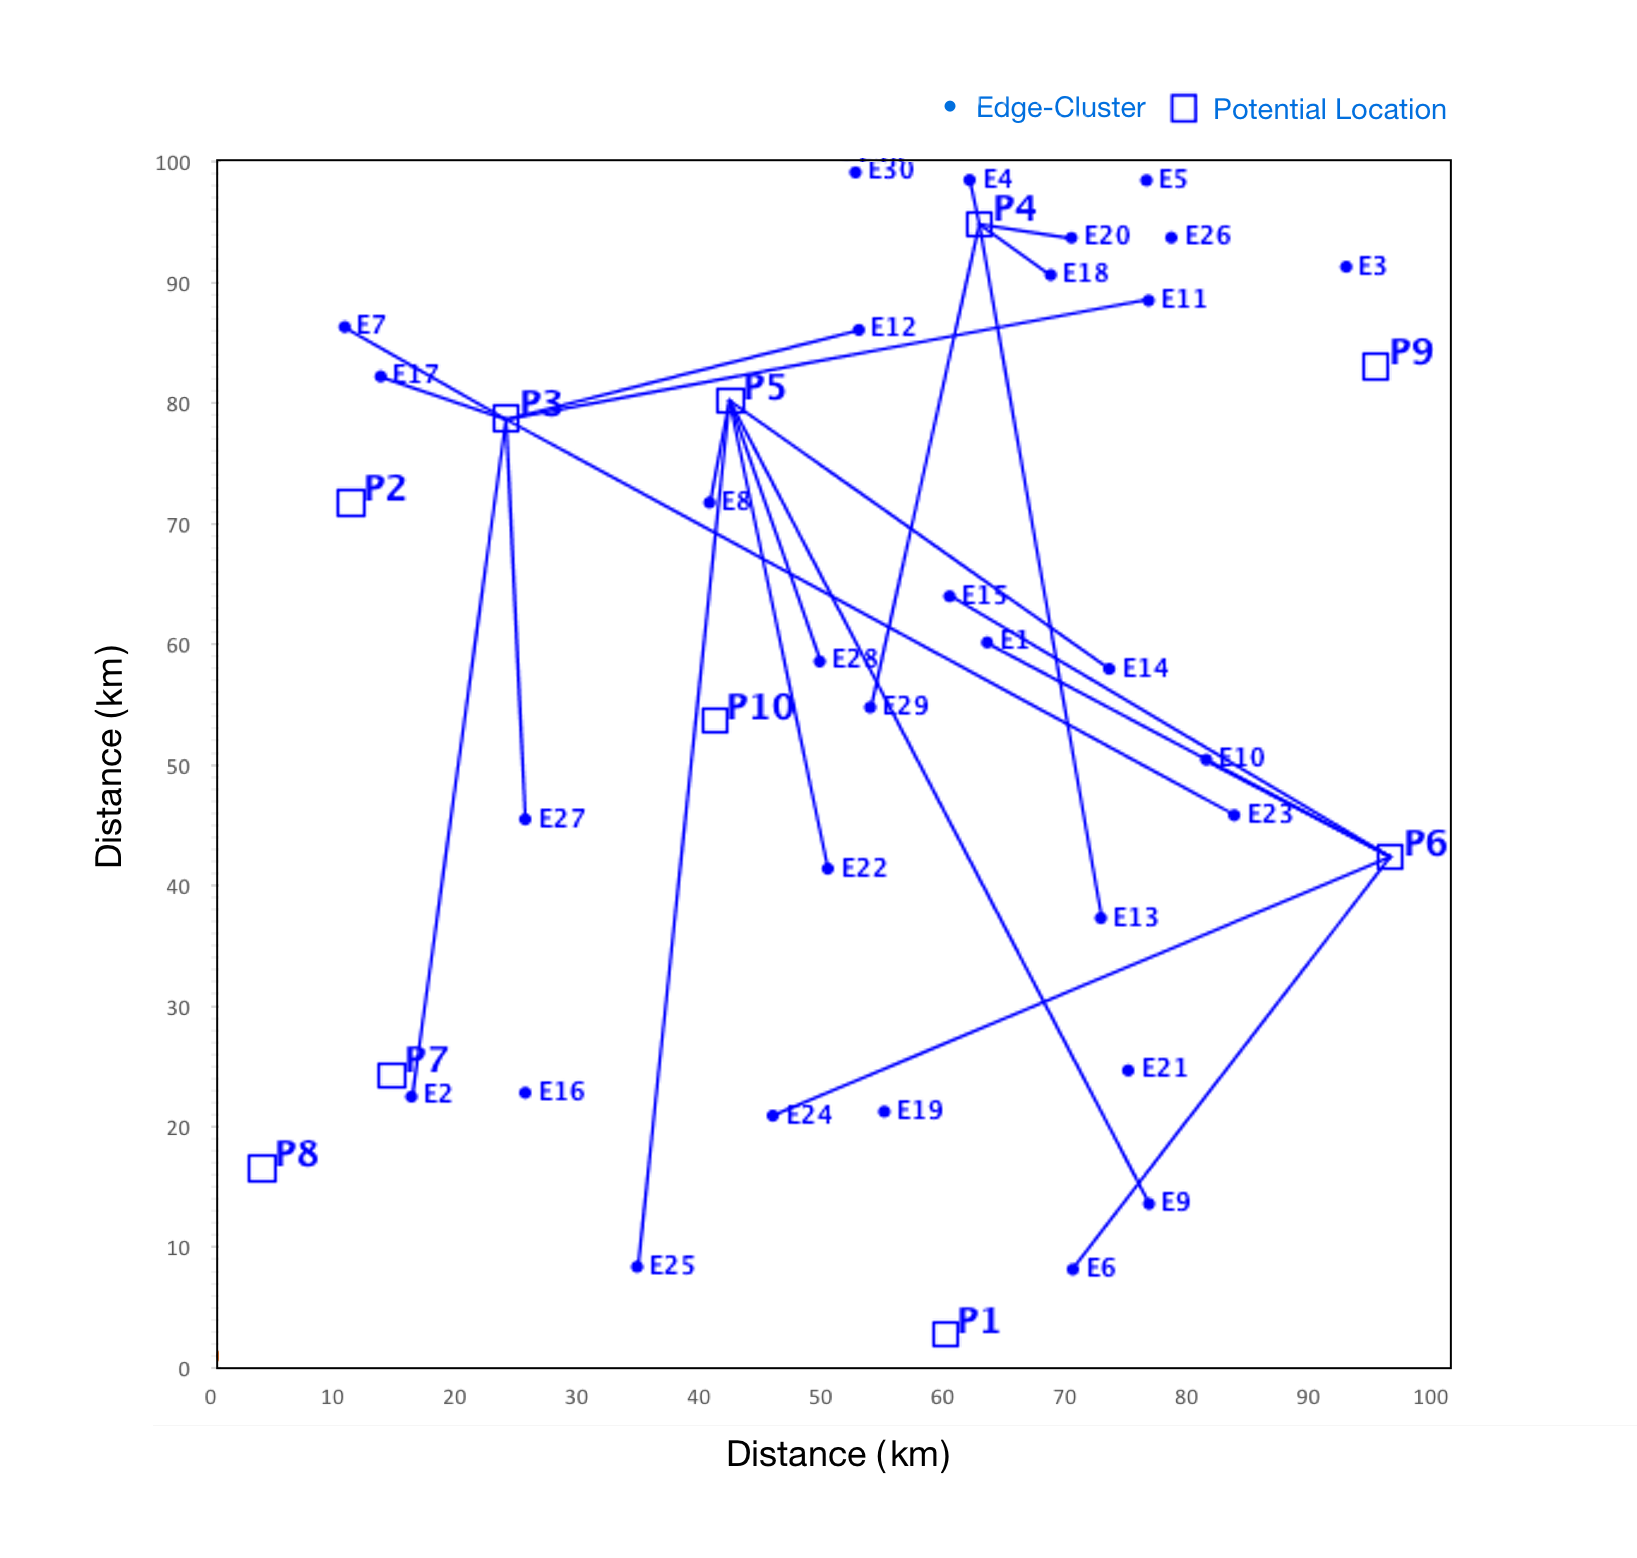
\includegraphics[trim=40 26 20 40,clip,width=.5\linewidth]{100x100problem_smpso2.png} \label{smpsorouting}}
\hfil
       % second figure itself
     %   \captionsetup{font={scriptsize,}}
        \subfloat[Planning result of PSONSGA, cost: \$1,004,900 delay: 322.7ms]
        {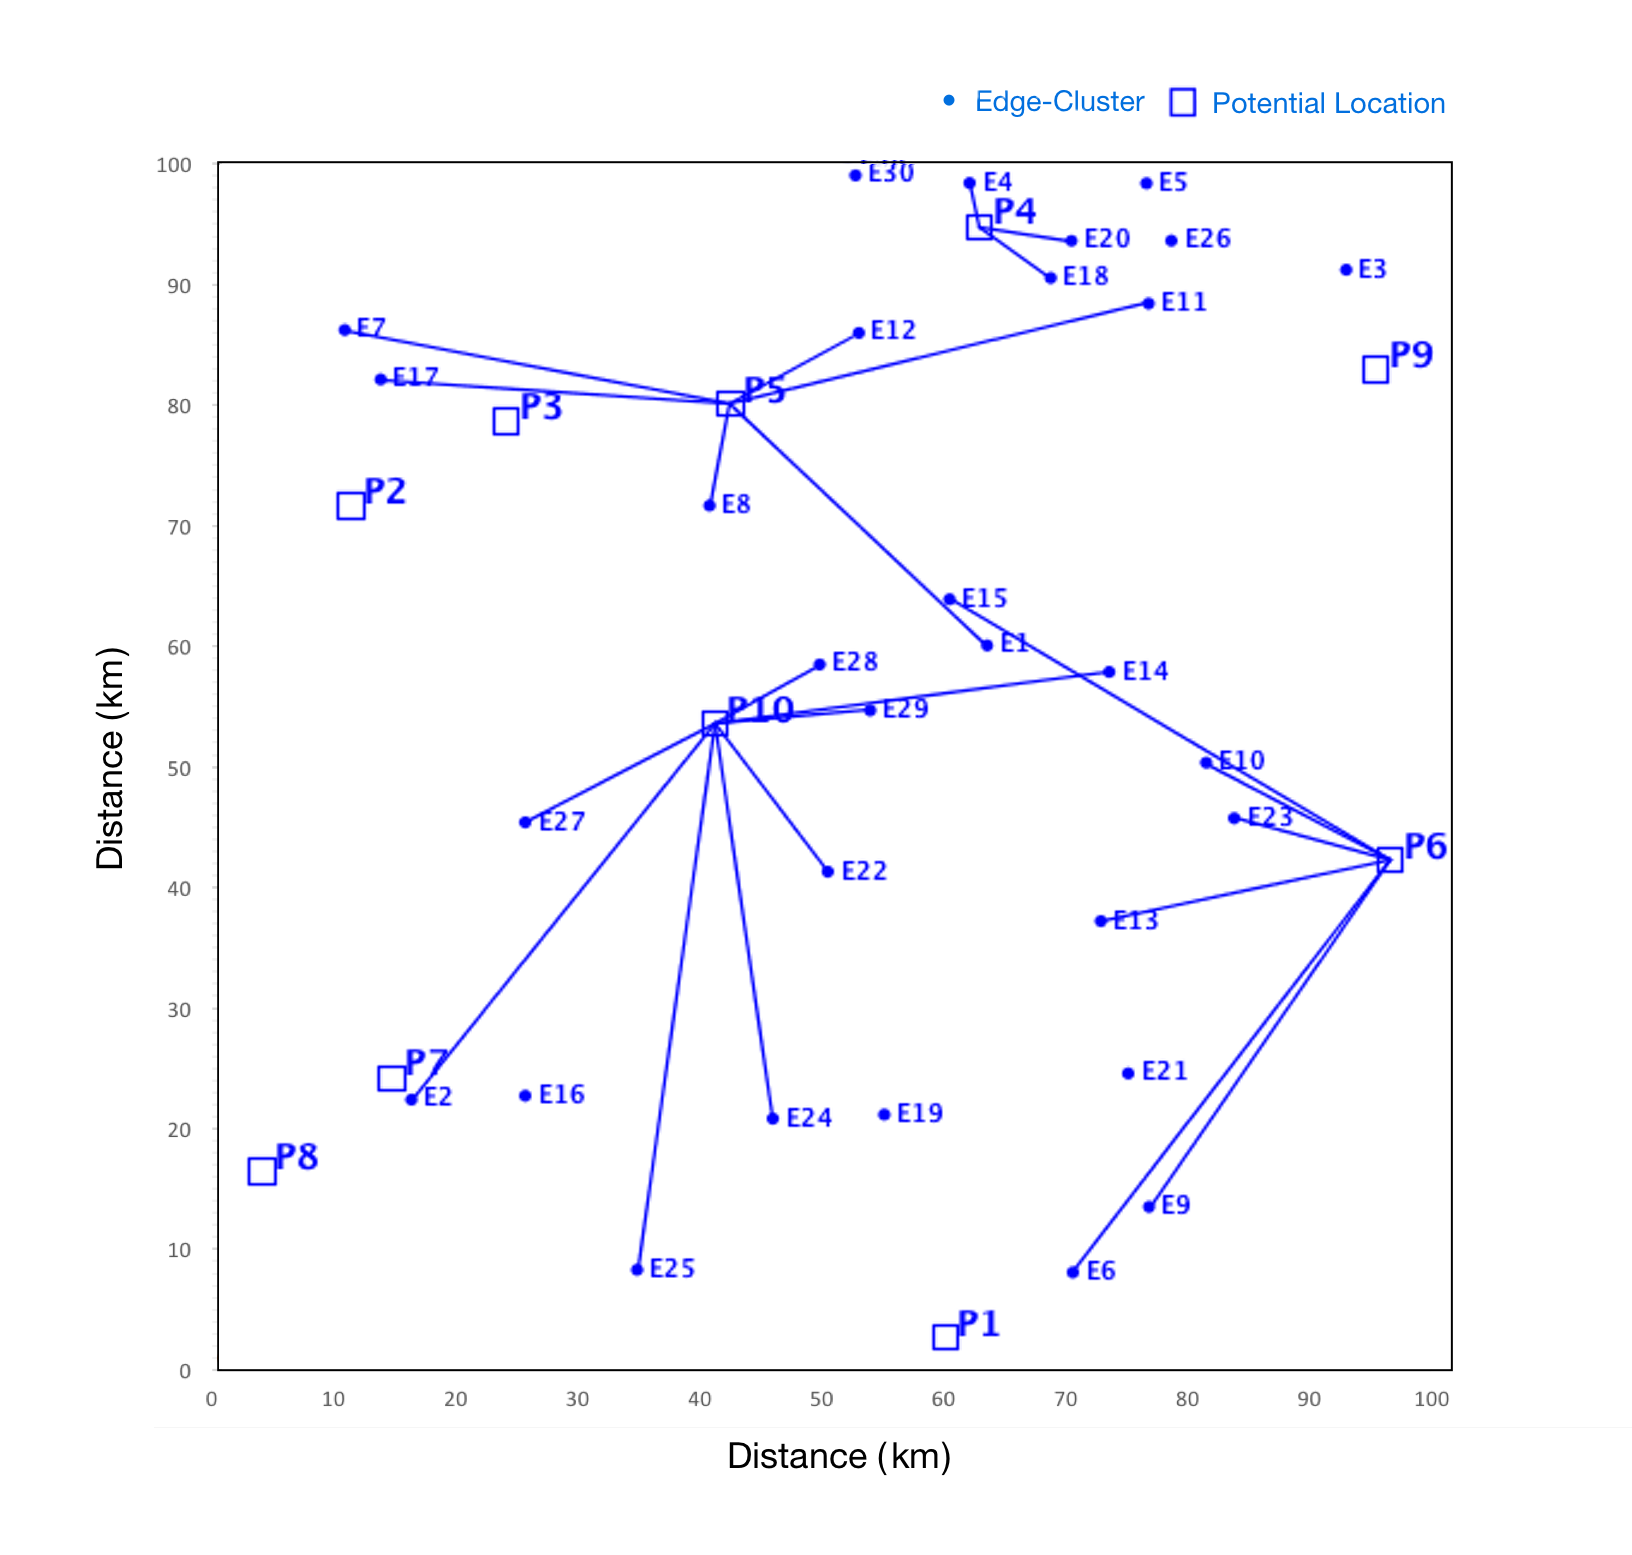
\includegraphics[trim=40 26 20 30,clip,width=.5\linewidth]{100x100problem_psonsga2.png}\label{psonsgarouting}}
    \caption{Planning result comparison}
\end{figure*}


The first column shows the solution number. The following two columns contain the cost and delay results obtained by the NSGA-II algorithm. Columns 4 and 5 provide, respectively, the decision variables for the link and fog type at each location, where ``0" indicates that no facility is installed, and subsequent numbers correspond to different facility types (fog or link). The following two columns show the CPLEX's results (cost and delay values). Since CPLEX only produces 7 solution frontiers, the non-existing solution rows are labelled as ``NA". Finally, the cost gaps and delay gaps between solutions from the NSGA-II and corresponding solution from the weighted sum is provided in the last two columns. 
The solution frontiers, for FPP3010 by applying NSGA-II, SMPSO, PSONSGA, are plotted in Figures \ref{nsgafro}, \ref{smpsofro} and \ref{psonsgafro}.



\begin{table}[h]
 % tabular material here
\caption{NSGA-II's solution set for FPP3010 (instance-1)}\label{table:solution.obj.nsgaii}
\centering
\resizebox{\columnwidth}{!}{
\tiny
\begin{tabular}{|*{9}{r|}}
\hline
 &\multicolumn{4}{|c|}{\textbf{NSGA-II}} &\multicolumn{2}{c|}{\textbf{Weighted Sum}} &&\\
 \hline
\textbf{Solution }&	\textbf{Cost }	&\textbf{Delay 	}	&\textbf{Variables-link}&\textbf{Variables-fog}&\textbf{Cost }	&\textbf{Delay }	&\textbf{Cost diff}	&\textbf{Delay diff}\\
\textbf{num}&	\textbf{ (\$)}	&\textbf{(ms)	}	&&&\textbf{(\$)}	&\textbf{ (ms)}	&\textbf{(\%) }	&\textbf{(\%)}\\

\hline

1	&121225	&   427.2	&0 0 0 0 0 0 0 0 0 1	&0 0 0 0 0 0 0 0 0 2	&			NA	&NA&&\\
2	&171225	&   410.8	&0 0 1 0 0 0 0 0 0 0	&0 0 3 0 0 0 0 0 0 0	&			NA	&NA&&\\
3	&239650	&   405.0	&1 0 1 0 0 0 0 0 0 0	&1 0 3 0 0 0 0 0 0 0	&			NA	&NA&&\\
4	&251225	&   383.7	&0 0 1 0 0 0 0 0 0 0	&0 0 4 0 0 0 0 0 0 0	&	      \cellcolor{blizzardblue} 251225&	\cellcolor{blizzardblue}383.7	&\cellcolor{blizzardblue}0	&\cellcolor{blizzardblue}0.00\%\\
5	&319650	&   383.1	&0 0 1 0 0 0 0 0 1 0	&0 0 4 0 0 0 0 0 1 0	&			NA	&NA&&\\
6	&372450	&   377.8	&0 0 1 0 0 0 0 0 1 0	&0 0 4 0 0 0 0 0 2 0	&			NA	&NA&&\\
7	&388075	&   377.6	&0 1 0 0 0 1 1 0 0 0	&0 1 0 0 0 1 4 0 0 0	&			NA	&NA&&\\
8	&422450	&   372.3	&0 0 1 0 0 0 0 0 0 1	&0 0 3 0 0 0 0 0 0 4	&			NA	&NA&&\\
9	&440875	&   372.2	&0 0 1 0 1 0 0 0 0 1	&0 0 1 0 2 0 0 0 0 4	&			NA	&NA&&\\
10	&490875	&   366.6	&1 0 1 0 0 0 0 0 0 1	&1 0 4 0 0 0 0 0 0 3	&			NA	&NA&&\\
11	&502450	&   356.2	&0 0 1 0 0 0 0 0 0 1	&0 0 4 0 0 0 0 0 0 4	&	      \cellcolor{blizzardblue} 502450	&\cellcolor{blizzardblue}356.1	&\cellcolor{blizzardblue}0	&\cellcolor{blizzardblue}0.03\%\\
12	&570875	&   355.5	&1 0 1 0 0 0 0 0 0 1	&1 0 4 0 0 0 0 0 0 4	&			NA	&NA&&\\
13	&623675	&   350.4	&1 0 1 1 0 0 0 0 0 0	&2 0 4 4 0 0 0 0 0 0	&			NA	&NA&&\\
14	&673675	&   350.0	&0 0 1 1 0 0 0 0 0 1	&0 0 3 4 0 0 0 0 0 4	&			NA	&NA&&\\
15	&692100	&   350.0	&0 1 0 0 0 0 1 0 1 1	&0 1 0 0 0 0 4 0 2 4	&			NA	&NA&&\\
16	&742100	&   344.5	&1 0 1 1 0 0 0 0 0 1	&1 0 4 3 0 0 0 0 0 4	&			NA	&NA&&\\
17	&753675	&   339.3	&0 0 1 1 0 0 0 0 0 1	&0 0 4 4 0 0 0 0 0 4	&			NA	&NA&&\\
18	&822100	&   338.8	&1 0 1 1 0 0 0 0 0 1	&1 0 4 4 0 0 0 0 0 4	&			NA	&NA&&\\
19	&874900	&   333.6	&1 0 1 1 0 0 0 0 0 1	&2 0 4 4 0 0 0 0 0 4	&			NA	&NA&&\\
20	&890525	&   333.4	&1 0 1 1 0 0 1 0 0 1	&1 0 4 4 0 0 1 0 0 4	&			NA	&NA&&\\
21	&924900	&   333.2	&0 0 1 1 1 0 0 0 0 1	&0 0 4 4 3 0 0 0 0 4	&			NA	&NA&&\\
22	&993325	&   327.6	&0 0 1 1 1 0 1 0 1 0	&0 0 3 4 4 0 4 0 1 0	&			NA	&NA&&\\
23	&1004900&   322.6	&0 0 1 1 1 0 0 0 0 1	&0 0 4 4 4 0 0 0 0 4	&	\cellcolor{blizzardblue}       1004900	&\cellcolor{blizzardblue}322.1&\cellcolor{blizzardblue}	0	&\cellcolor{blizzardblue}0.17\%\\
24	&1073325&   322.0	&0 0 1 1 1 0 1 0 1 0	&0 0 4 4 4 0 4 0 1 0	&			NA	&NA&&\\
25	&1141750&   321.8	&1 1 0 1 0 1 1 0 0 1	&1 1 0 4 0 4 4 0 0 4	&			NA	&NA&&\\
26	&1176125&   317.1	&0 0 1 1 1 0 1 0 1 0	&0 0 4 4 4 0 4 0 3 0	&			NA	&NA&&\\
27	&1244550&   316.4	&1 0 1 1 1 0 1 0 1 0	&3 0 1 4 4 0 4 0 4 0	&			NA	&NA&&\\
28	&1256125&   311.5	&0 0 1 1 0 0 1 0 1 1	&0 0 4 4 0 0 4 0 4 4	&			NA	&NA&&\\
29	&1324550&   311.3	&1 1 0 1 0 1 1 0 0 1	&1 4 0 4 0 4 4 0 0 4	&			NA	&NA&&\\
30	&1377350&   311.2	&1 0 0 1 1 1 1 0 1 0	&2 0 0 4 4 4 4 0 4 0	&			NA	&NA&&\\
31	&1392975&   311.0	&1 1 0 1 1 1 1 0 0 1	&1 4 0 4 1 4 4 0 0 4	&			NA	&NA&&\\
32	&1415775&   311.0	&0 1 0 1 1 1 1 1 0 1	&0 4 0 4 3 4 3 1 0 4	&			NA	&NA&&\\
33	&1445775&   310.9	&1 0 1 1 1 1 1 0 1 0	&2 0 1 4 4 4 4 0 4 0	&			NA	&NA&&\\
34	&1495775&   306.1	&1 0 1 1 1 1 1 0 1 0	&3 0 1 4 4 4 4 0 4 0	&			NA	&NA&&\\
35	&1507350&   305.6	&0 0 1 1 1 0 1 0 1 1	&0 0 4 4 4 0 4 0 4 4	&	  \cellcolor{blizzardblue}     1507350	&\cellcolor{blizzardblue}299.9	&\cellcolor{blizzardblue}0	&\cellcolor{blizzardblue}1.87\%\\
36	&1575775&   301.3	&1 0 1 1 1 0 1 0 1 1	&1 0 4 4 4 0 4 0 4 4	&			NA	&NA&&\\
37	&1628575&   300.6	&1 0 1 1 0 1 1 0 1 1	&4 0 4 4 0 2 4 0 4 4	&			NA	&NA&&\\
38	&1678575&   300.2	&1 0 1 1 1 0 1 0 1 1	&3 0 4 4 4 0 4 0 4 4	&			NA	&NA&&\\
39	&1697000&   300.1	&1 1 0 1 1 1 1 0 1 1	&4 4 0 4 4 4 1 0 4 2	&			NA	&NA&&\\
40	&1747000&   299.9	&1 1 0 1 1 1 1 0 1 1	&4 4 0 4 4 4 1 0 4 3	&			NA	&NA&&\\
41	&1758575&   295.1	&1 0 1 1 1 0 1 0 1 1	&4 0 4 4 4 0 4 0 4 4	&			NA	&NA&&\\
42	&1827000&   294.6	&1 0 1 1 1 1 1 0 1 1	&4 0 4 4 4 1 4 0 4 4	&			NA	&NA&&\\
43	&1929800&   292.0	&1 0 1 1 1 1 1 0 1 1	&4 0 4 4 3 4 4 0 4 4	&			NA	&NA&&\\
44	&1998225&   289.8	&1 1 1 1 1 1 1 0 1 1	&4 1 4 4 4 4 4 0 4 3	&			NA	&NA&&\\
45	&2009800&   289.2	&1 0 1 1 1 1 1 0 1 1	&4 0 4 4 4 4 4 0 4 4	&			NA	&NA&&\\
46	&2078225&   289.0	&1 1 1 1 1 1 1 0 1 1	&4 1 4 4 4 4 4 0 4 4	&	     \cellcolor{blizzardblue}  2078225	&\cellcolor{blizzardblue}283.2	&\cellcolor{blizzardblue}0&\cellcolor{blizzardblue}	2.03\%\\
47	&2181025&   284.5	&1 0 1 1 1 1 1 1 1 1	&4 0 4 3 4 4 4 4 4 4	&	      \cellcolor{blizzardblue} 2148225.151&	\cellcolor{blizzardblue}282.8	&\cellcolor{blizzardblue}-0.015038731	&\cellcolor{blizzardblue}0.60\%\\
48	&2249450&   284.4	&1 1 1 1 1 1 1 1 1 1	&4 1 4 3 4 4 4 4 4 4	&	      \cellcolor{blizzardblue} 2586500	&\cellcolor{blizzardblue}282.7	&\cellcolor{blizzardblue}0.149836627	&\cellcolor{blizzardblue}0.61\%\\
49	&2261025&   284.1	&1 0 1 1 1 1 1 1 1 1	&4 0 4 4 4 4 4 4 4 4	&			NA&	NA&&\\
\hline
\end{tabular}}
\end{table}

\iffalse
\begin{table}[H]
 % tabular material here
%\caption{NSGA-II's solution set for FPP3010 (instance-1)}\label{table:solution.obj.nsgaii}
\centering
\resizebox{\textwidth}{!}{
\footnotesize
\begin{tabular}{|*{9}{r|}}
\hline
 &\multicolumn{4}{|c|}{\textbf{NSGA-II}} &\multicolumn{2}{c|}{\textbf{Weighted Sum}} &&\\
 \hline
\textbf{Solution }&	\textbf{Cost }	&\textbf{Delay 	}	&\textbf{Variables-link}&\textbf{Variables-fog}&\textbf{Cost }	&\textbf{Delay }	&\textbf{Cost diff}	&\textbf{Delay diff}\\
\textbf{num}&	\textbf{ (\$)}	&\textbf{(ms)	}	&&&\textbf{(\$)}	&\textbf{ (ms)}	&\textbf{(\%) }	&\textbf{(\%)}\\

\hline


29	&1324550&   311.3	&1 1 0 1 0 1 1 0 0 1	&1 4 0 4 0 4 4 0 0 4	&			NA	&NA&&\\
30	&1377350&   311.2	&1 0 0 1 1 1 1 0 1 0	&2 0 0 4 4 4 4 0 4 0	&			NA	&NA&&\\
31	&1392975&   311.0	&1 1 0 1 1 1 1 0 0 1	&1 4 0 4 1 4 4 0 0 4	&			NA	&NA&&\\
32	&1415775&   311.0	&0 1 0 1 1 1 1 1 0 1	&0 4 0 4 3 4 3 1 0 4	&			NA	&NA&&\\
33	&1445775&   310.9	&1 0 1 1 1 1 1 0 1 0	&2 0 1 4 4 4 4 0 4 0	&			NA	&NA&&\\
34	&1495775&   306.1	&1 0 1 1 1 1 1 0 1 0	&3 0 1 4 4 4 4 0 4 0	&			NA	&NA&&\\
35	&1507350&   305.6	&0 0 1 1 1 0 1 0 1 1	&0 0 4 4 4 0 4 0 4 4	&	       1507350	&299.9	&0	&1.87\%\\
36	&1575775&   301.3	&1 0 1 1 1 0 1 0 1 1	&1 0 4 4 4 0 4 0 4 4	&			NA	&NA&&\\
37	&1628575&   300.6	&1 0 1 1 0 1 1 0 1 1	&4 0 4 4 0 2 4 0 4 4	&			NA	&NA&&\\
38	&1678575&   300.2	&1 0 1 1 1 0 1 0 1 1	&3 0 4 4 4 0 4 0 4 4	&			NA	&NA&&\\
39	&1697000&   300.1	&1 1 0 1 1 1 1 0 1 1	&4 4 0 4 4 4 1 0 4 2	&			NA	&NA&&\\
40	&1747000&   299.9	&1 1 0 1 1 1 1 0 1 1	&4 4 0 4 4 4 1 0 4 3	&			NA	&NA&&\\
41	&1758575&   295.1	&1 0 1 1 1 0 1 0 1 1	&4 0 4 4 4 0 4 0 4 4	&			NA	&NA&&\\
42	&1827000&   294.6	&1 0 1 1 1 1 1 0 1 1	&4 0 4 4 4 1 4 0 4 4	&			NA	&NA&&\\
43	&1929800&   292.0	&1 0 1 1 1 1 1 0 1 1	&4 0 4 4 3 4 4 0 4 4	&			NA	&NA&&\\
44	&1998225&   289.8	&1 1 1 1 1 1 1 0 1 1	&4 1 4 4 4 4 4 0 4 3	&			NA	&NA&&\\
45	&2009800&   289.2	&1 0 1 1 1 1 1 0 1 1	&4 0 4 4 4 4 4 0 4 4	&			NA	&NA&&\\
46	&2078225&   289.0	&1 1 1 1 1 1 1 0 1 1	&4 1 4 4 4 4 4 0 4 4	&	       2078225	&283.2	&0&	2.03\%\\
47	&2181025&   284.5	&1 0 1 1 1 1 1 1 1 1	&4 0 4 3 4 4 4 4 4 4	&	       2148225.151&	282.8	&-0.015038731	&0.60\%\\
48	&2249450&   284.4	&1 1 1 1 1 1 1 1 1 1	&4 1 4 3 4 4 4 4 4 4	&	       2586500	&282.7	&0.149836627	&0.61\%\\
49	&2261025&   284.1	&1 0 1 1 1 1 1 1 1 1	&4 0 4 4 4 4 4 4 4 4	&			NA&	NA&&\\
\hline
\end{tabular}}
\end{table}
\fi
%As written in Chapter 4, evolutionary algorithms first initializes a population of solution points, then it iteratively updating the population by crossover, mutation or velocity updating operations, and finally evaluates and selects the fittest solutions as the output solution sets.

 
To better understand the results, we select the solution number 23 from Table \ref{table:solution.obj.nsgaii} (cost: \$1,004,900, delay: 322.1ms) and plot the corresponding topology for this result in \Fig{nsgarouting}. The result for the same expense (i.e. \$1,004,900) from Weighted sum, SMPSO and PSONSGA are also plotted respectively, in Figures \ref{CPLEXrouting}, \ref{smpsorouting} and \ref{psonsgarouting}. The detailed examination shows that both NSGA and PSONSGA generate the same fog network setup (fog node placement, fog node selection, and link selection) as the exact algorithm (weighted sum). For the same capital expenditure, the results from Weighted sum, NSGA-II, SMPSO and PSONSGA give 322.1ms, 322.6ms, 323.8ms and 322.7ms delay respectively. The minor delay differences are due to the misplacement of a small number of edge-clusters (see E11 and E12 for example). These differences can be compensated through user-relocation and load-balancing schemes. This topic has been thoroughly researched in cloud computing, and mature research results can be applied on this relocation subproblem.




\iffalse
Before we apply evolutionary heuristic algorithm: NSGAII \cite{Deb:2002:FEM:2221359.2221582} and SMPSO\cite{smpso} on FPP problem. 
we need to determine the best parameter setting for our specific MOCO problem. We use three quality indicators to evaluate the performance between different settings. 
These three quality indicators are Epsilon\cite{Zitzler:2003:PAM:2221365.2221632}, Spread\cite{Deb:2002:FEM:2221359.2221582} and Hyper-volume\cite{Auger:2009:THI:1527125.1527138}. 
Epsilon Indicator \cite{Zitzler:2003:PAM:2221365.2221632} evaluates the smallest amount $\epsilon$ that it needs to translate the set A (solution set we computed) so that every point in B (reference front, can be true Pareto front) is covered.
Spread Indicator evaluates the euclidean distance between consecutive solutions within solution front.
Hyper-volume\cite{Auger:2009:THI:1527125.1527138}indicator gives the volume covered by members of a non-dominated set of solutions in the objective space.
For same problem instance: \textit{30-10}, we run 10 independent tests for each setting in NSGAII and SMPSO. After analyzing the variance on the Epsilon, Spread and Hyper-volume, we choose best performance setting which shows in table \ref{nsgaparatable}


\begin{figure*}[!t]
\centering
\subfloat[NSGAII Quality Indicator for Different Mutation Index Configuration]{\includegraphics[page=1,width=7.5in]{Sep_9_NSGAII_Mutation_Index_3010.png}\label{nsgaidx}}
\caption{NSGAII Quality Indicator} 
\end{figure*}
\begin{figure*}[!t]
\centering{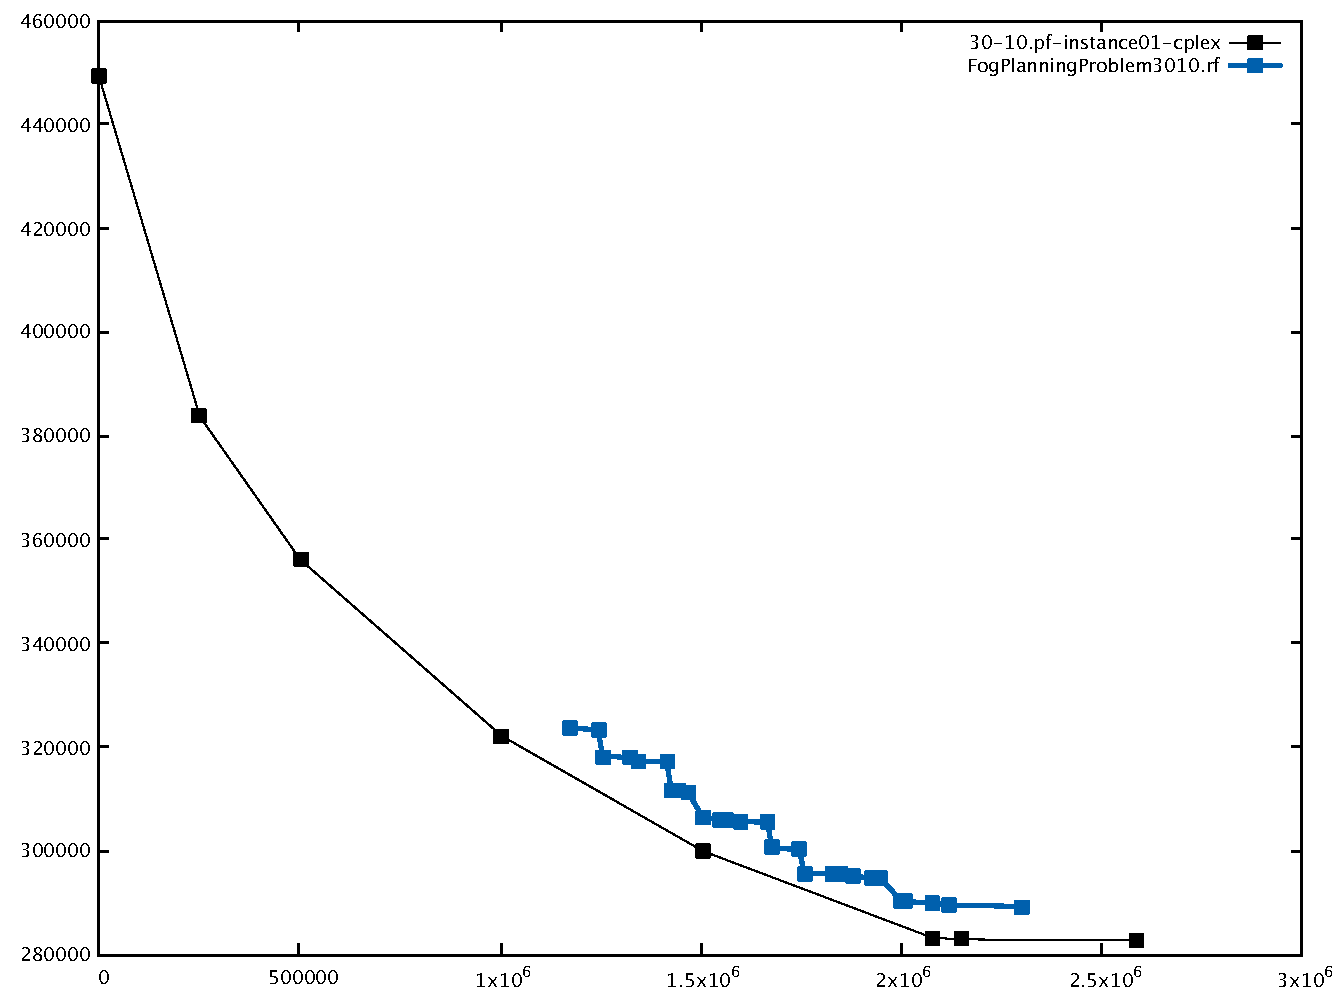
\includegraphics[page=1,width=3.5in]{nsgamuidx_3010.pdf}
\label{nsgaidx}}
\caption{Best NSGAII Setting's Pareto Front Result} 
\end{figure*}

\begin{figure*}[!t]
\centering
\subfloat[NSGAII Quality Indicator for Different Population Configuration]{\includegraphics[page=1,width=7.5in]{Sep_9_NSGAII_Popu_3010.png}
\label{nsgaidx}}
\caption{NSGAII Quality Indicator} 
\end{figure*}
\begin{figure*}[!t]
\centering{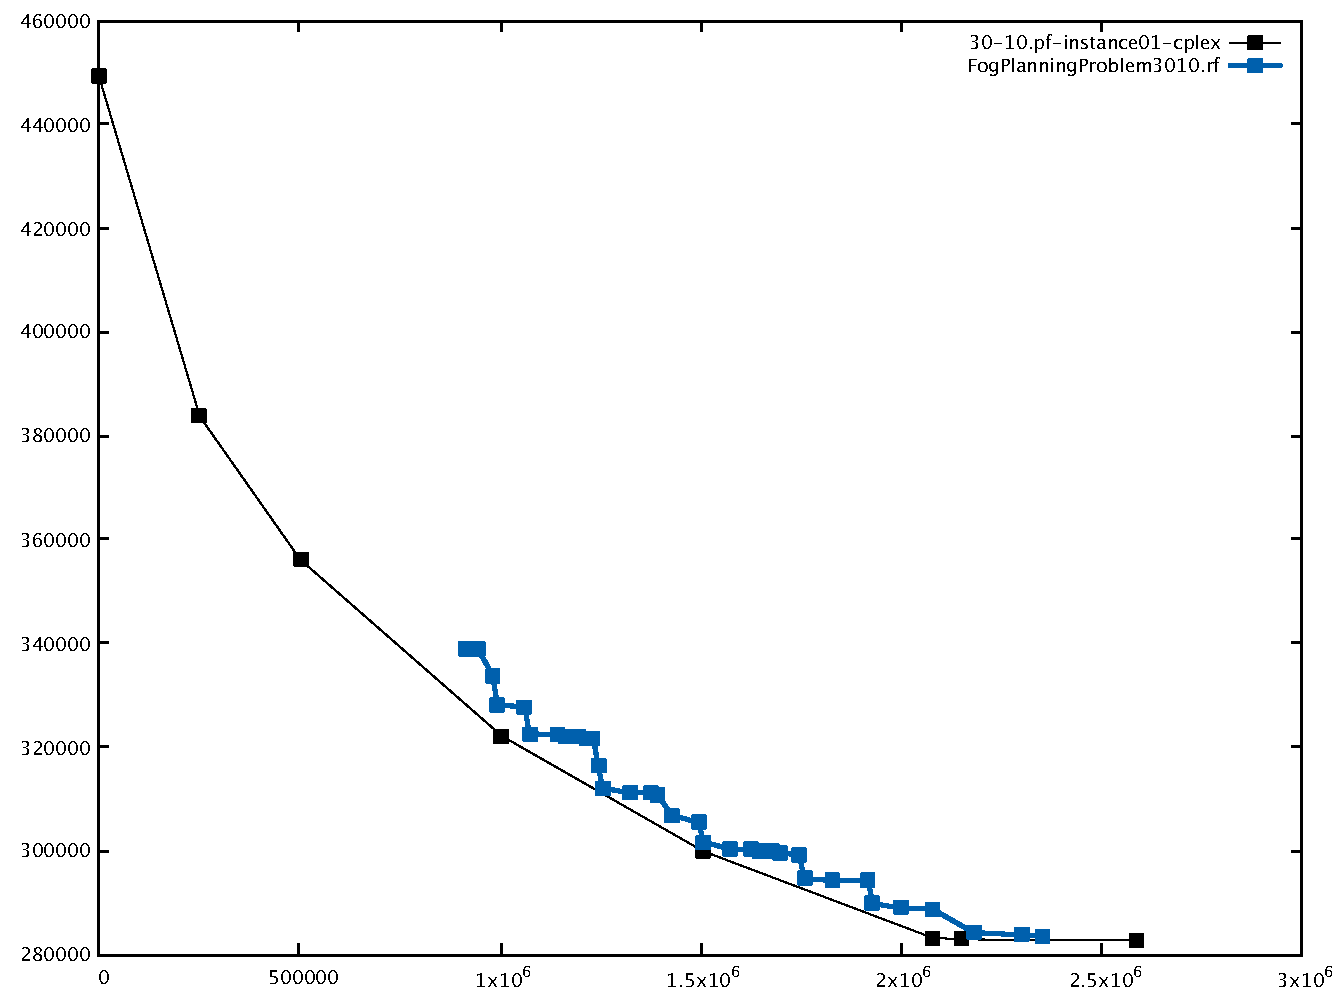
\includegraphics[page=1,width=3.5in]{nsga_pop_3010.pdf}
\label{nsgaidx}}
\caption{Best NSGAII Setting's Pareto Front Result} 
\end{figure*}

\begin{table}[H]
\caption{NSGAII Parameter Selection}
\label{nsgaparatable}
\centering
\resizebox{\linewidth}{!}{%
\begin{tabular}{ l r r r }
  \toprule
  NSGAII parameter choice & Experiment group & &Final choice \\
  \midrule
  Mutation Distribution Index & 2,4,6,...,18,20 && 20 \\
  Mutation Probability & && $ 1 / \textit{number of variable}$\\
  Crossover Distribution Index & 2,4,6,...,18,20 && 20\\
  Crossover Probability & 0.5,0.6,...,0.9&& 0.9\\
  Population & 100,200,...,1000 && 1000 \\
  \bottomrule
\end{tabular}}
\end{table}

As we can see, the results NSGAII produced, show good convergence to true Pareto Front and gives far more solutions than simple weighted-sum algorithm produced. However, its Pareto front can only cover part of the total Pareto front. Even if we increase the max iteration as shown in \Fig{nsgaitertest}, there still no improvement in view of coverage. 

The \Fig{nsgaitertest} shows the result of running NSGAII on (30-10) FPP problem, with best parameter settings from previous experiment (Table \ref{nsgaparatable}) undergoing \{1000, 1500, 2000, ..., 5500\} iterations. No obvious coverage improvement perceived.
The reason behind this is, NSGAII's solutions is highly dependent on the initial solutions. As can be seen in \Fig{nsgaini}. NSGAII algorithm starts its iteration from a set of random generated initial solutions. Without prior knowledge of searching domain. NSGAII algorithm and its non-dominated sorting mechanism will restrict the solution from exploring uncharted territory. New territory solution tends to fall behind in dominating ranking, and more likely to be discarded. We will give solution to deal with this drawback in PSONSGAII section. 
\begin{figure}[H]
\centerline{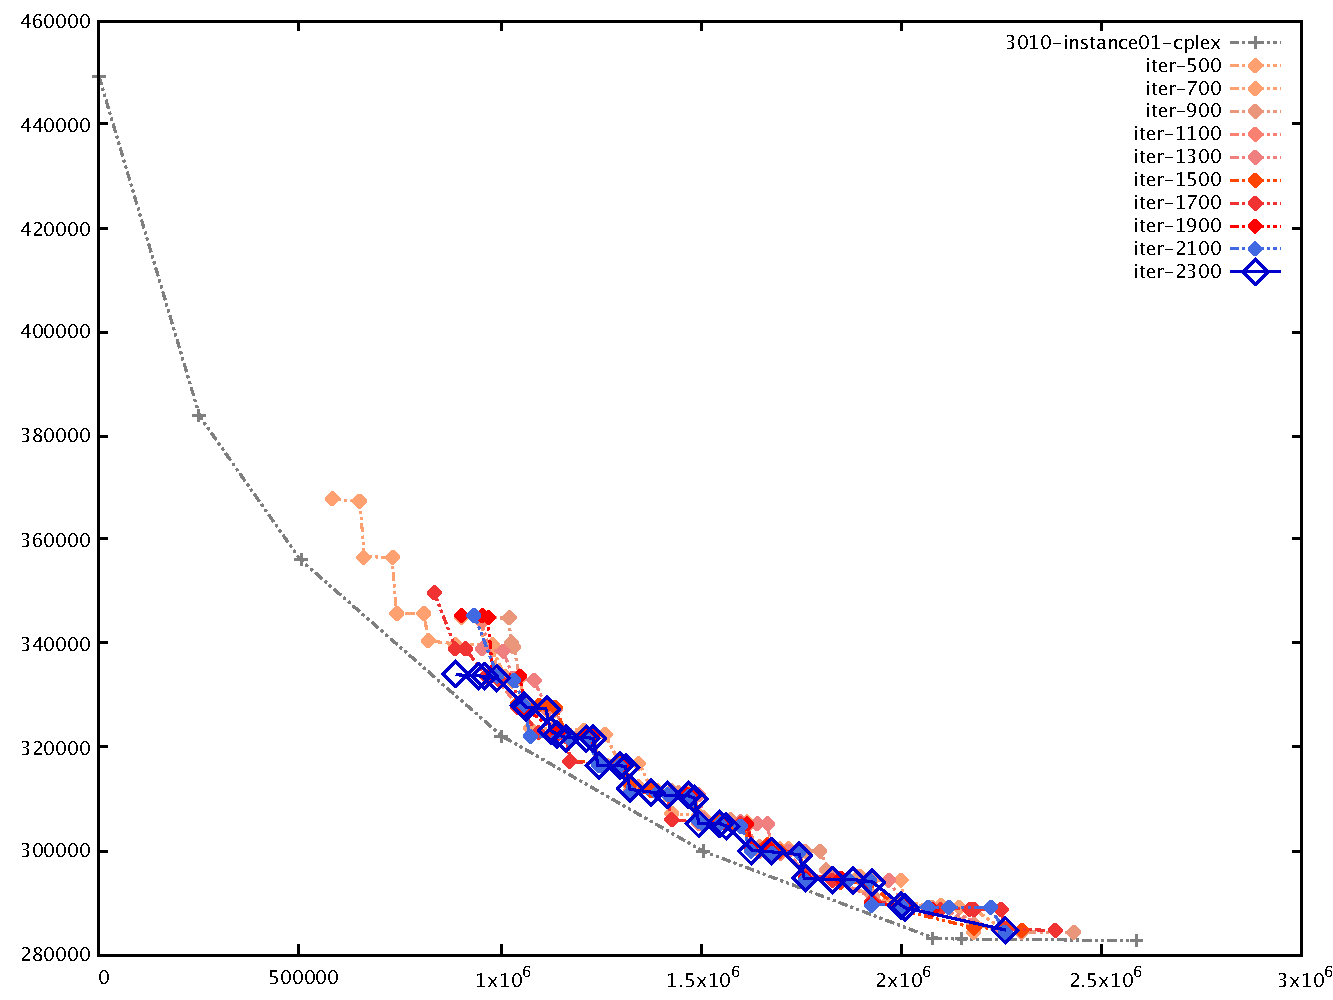
\includegraphics[page=1,width=3.5in]{nsgaitertest.pdf}}
\caption{NSGAII Iteration Test} 
\label{nsgaitertest}
\end{figure}
\begin{figure}[H]
\centerline{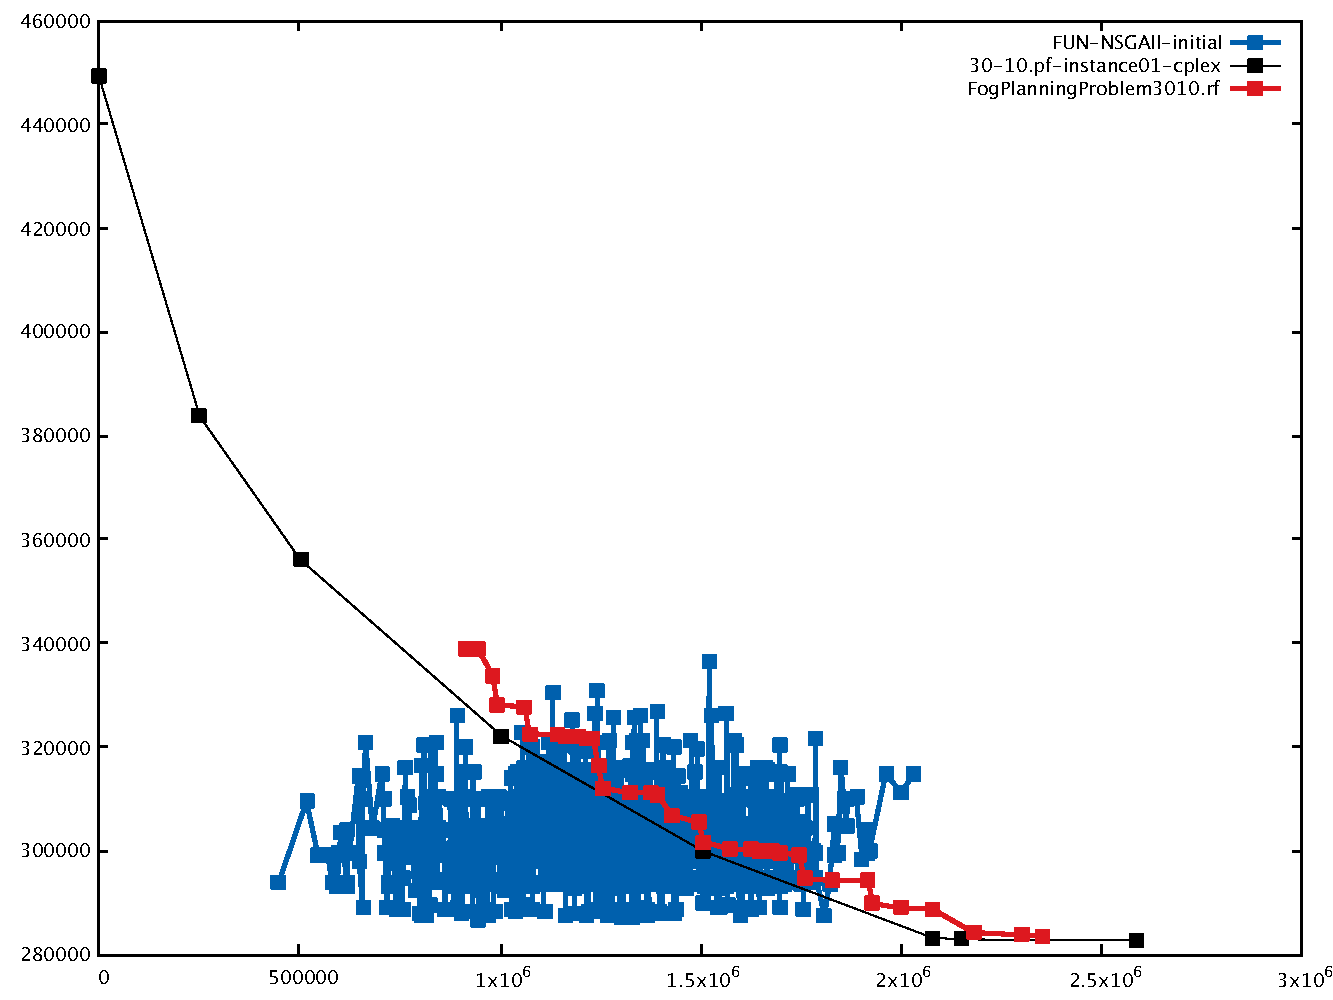
\includegraphics[page=1,width=3.5in]{nsga-initial.pdf}}
\caption{NSGAII Initial vs Output Front} 
\label{nsgaini}
\end{figure}

\subsection{Speed-constrained Multi-objective Particle Swarm Algorithm}\label{smpso}




%\begin{figure*}[!t]
%\centering
%\subfloat[Case I]{\includegraphics[width=2.5in]{box}%
%\label{fig_first_case}}
%\hfil
%\subfloat[Case II]{\includegraphics[width=2.5in]{box}%
%\label{fig_second_case}}
%\caption{Simulation results for the network.}
%\label{fig_sim}
%\end{figure*}

\begin{figure*}[!t]
\centering
\subfloat[SMPSO with Different Mutation Distribution Index]{\includegraphics[page=1,width=7.5in]{Sep_10_SMPSOMutationIndex_3010.png}%
\label{psomtidx}}
\caption{SMPSO Quality Indicator} 
\end{figure*}
\begin{figure*}[!t]
\centering{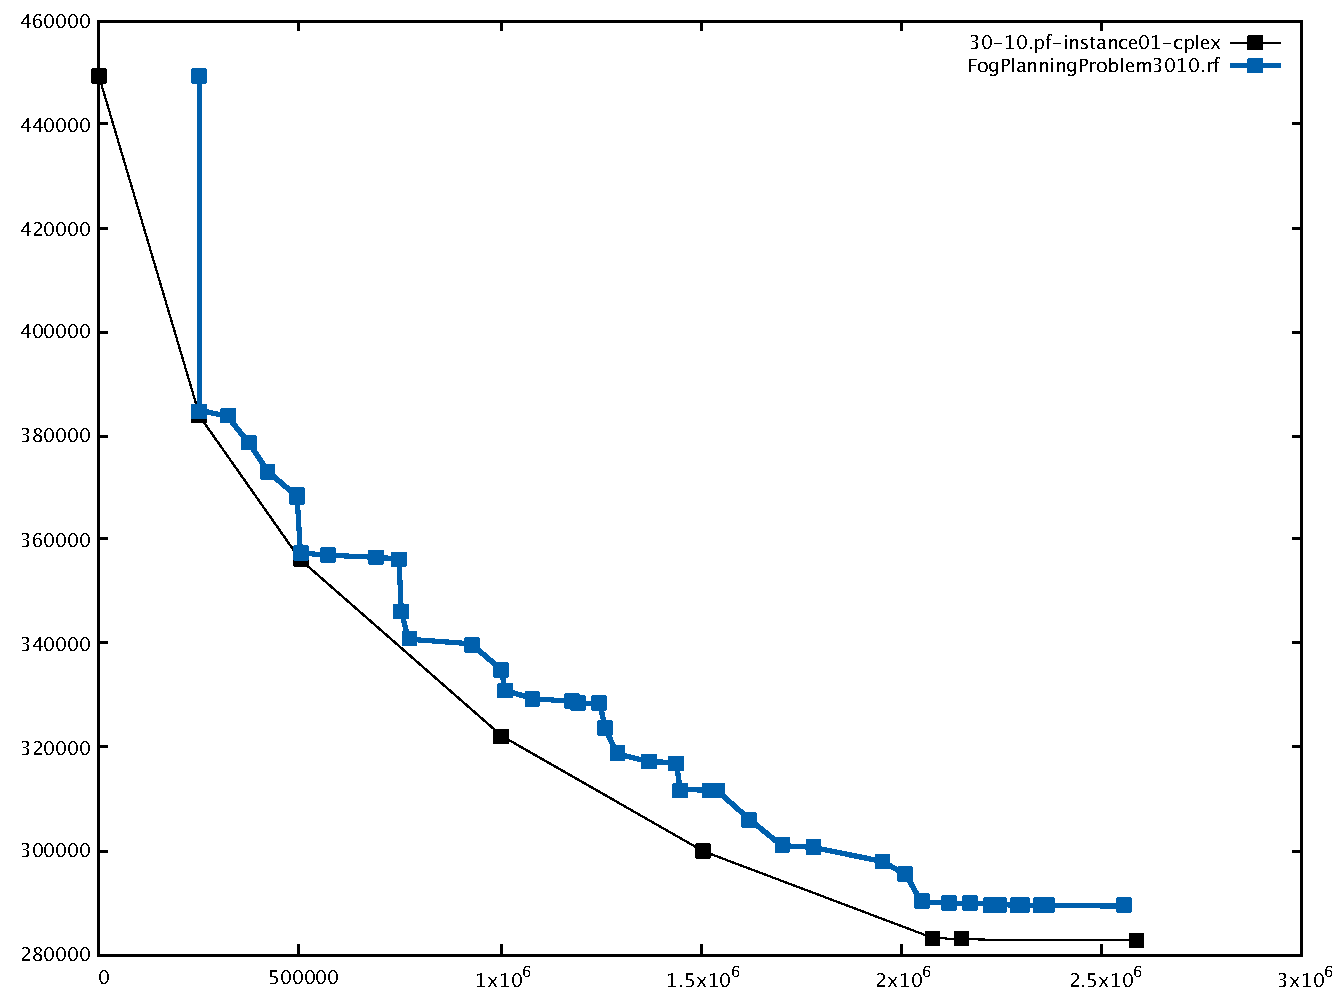
\includegraphics[page=1,width=3.5in]{smpso-mutidx-3010.pdf}
\label{psobest}}
\caption{Best SMPSO Setting's Pareto Front Result} 
\end{figure*}

\begin{figure*}[!t]
\centering
\subfloat[SMPSO with Different Swarm Size]{\includegraphics[page=1,width=7.5in]{Sep_10_SMPSOSwarmsize_3010}
\label{psoss}}
\caption{SMPSO Quality Indicator} 
\end{figure*}
\begin{figure*}[!t]
\centering
\subfloat[]{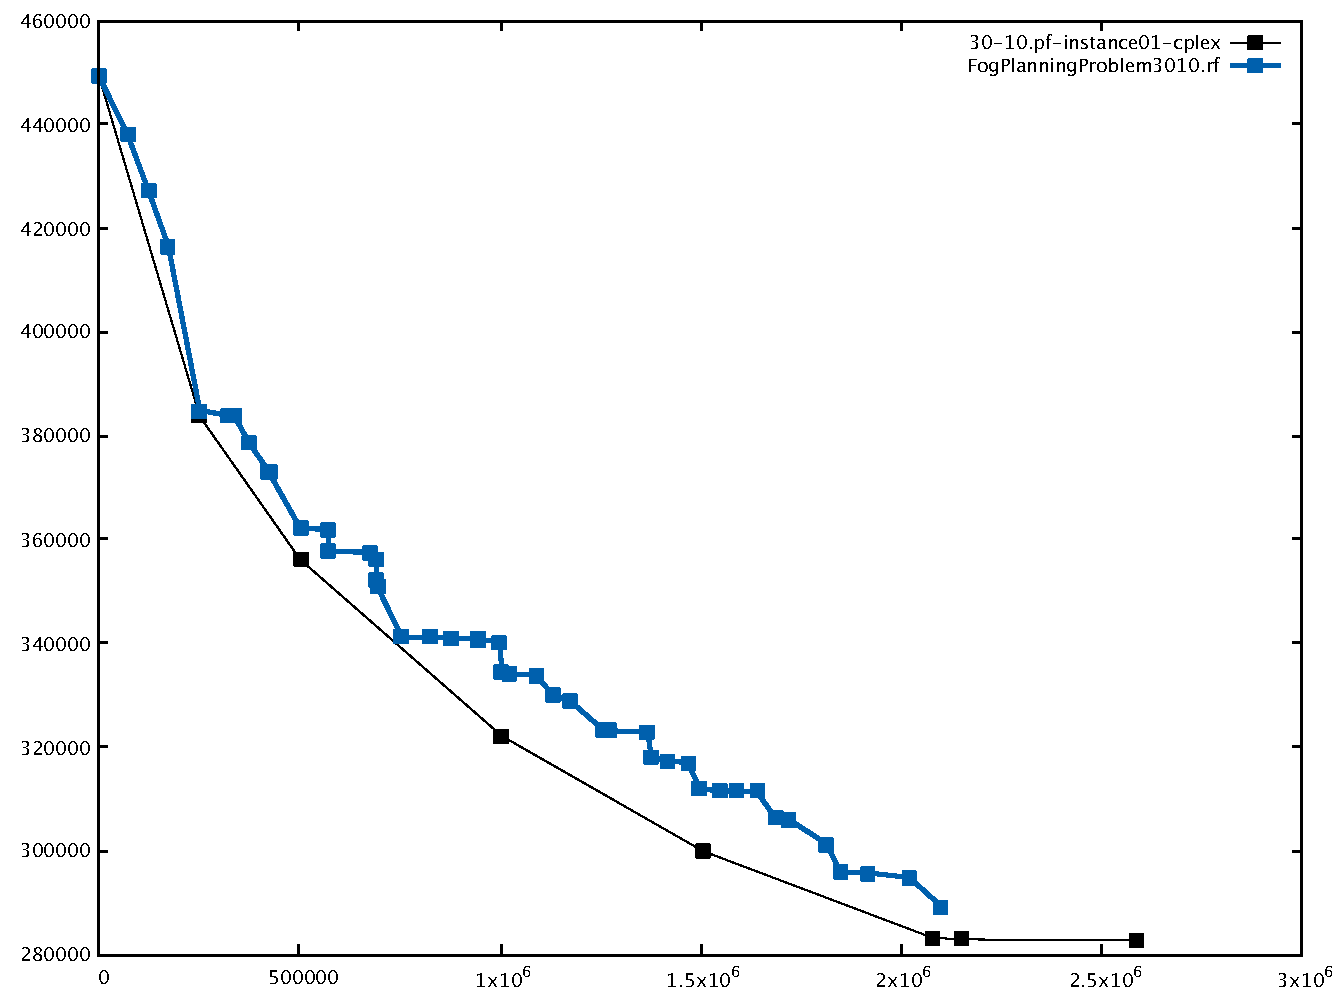
\includegraphics[page=1,width=3.5in]{SMPSO-swarmsize-3010.pdf}
\label{psobest2}}
\caption{Best SMPSO Setting (Swarm Size)'s Pareto Front Result} 
\end{figure*}

\begin{table}[H]
\caption{SMPSO Parameter Selection}
\label{smpsoparatable}
\centering
\resizebox{\linewidth}{!}{%
\begin{tabular}{ l r r r }
  \toprule
  SMPSO parameter choice & Experiment group & &Final choice \\
  \midrule
  Mutation Distribution Index & 2,4,6,...,18,20 && 18 \\
  Mutation Probability & && $ 1 / \textit{number of variable}$\\
  Crossover Distribution Index & 2,4,6,...,18,20 && 20\\
  Crossover Probability & 0.5,0.6,...,0.9 && 0.9\\
  Swarm Size & 100,200,...,1000 && 1000 \\
  \bottomrule
\end{tabular}}
\end{table}

As we can see, the results that SMPSO produced, show good coverage of whole Pareto Front. However, its Pareto front struggle to converge to the true Pareto front. Even if we increase the max iteration as shown in \Fig{smpsoitertest}, there still a gap between SMPSO solutions to true Pareto front. 

The \Fig{smpsoitertest} shows the result of running SMPSO on (30-10) FPP problem, with best parameter settings from previous experiment (Table \ref{smpsoparatable}) undergoing \{1000, 1500, 2000, ..., 5500\} iterations. Although there is convergence improvement giving more iteration running. The 5500 iteration running result is still inferior than counterpart result from NSGAII algorithm convergence-wise.


\begin{figure}[H]
\centerline{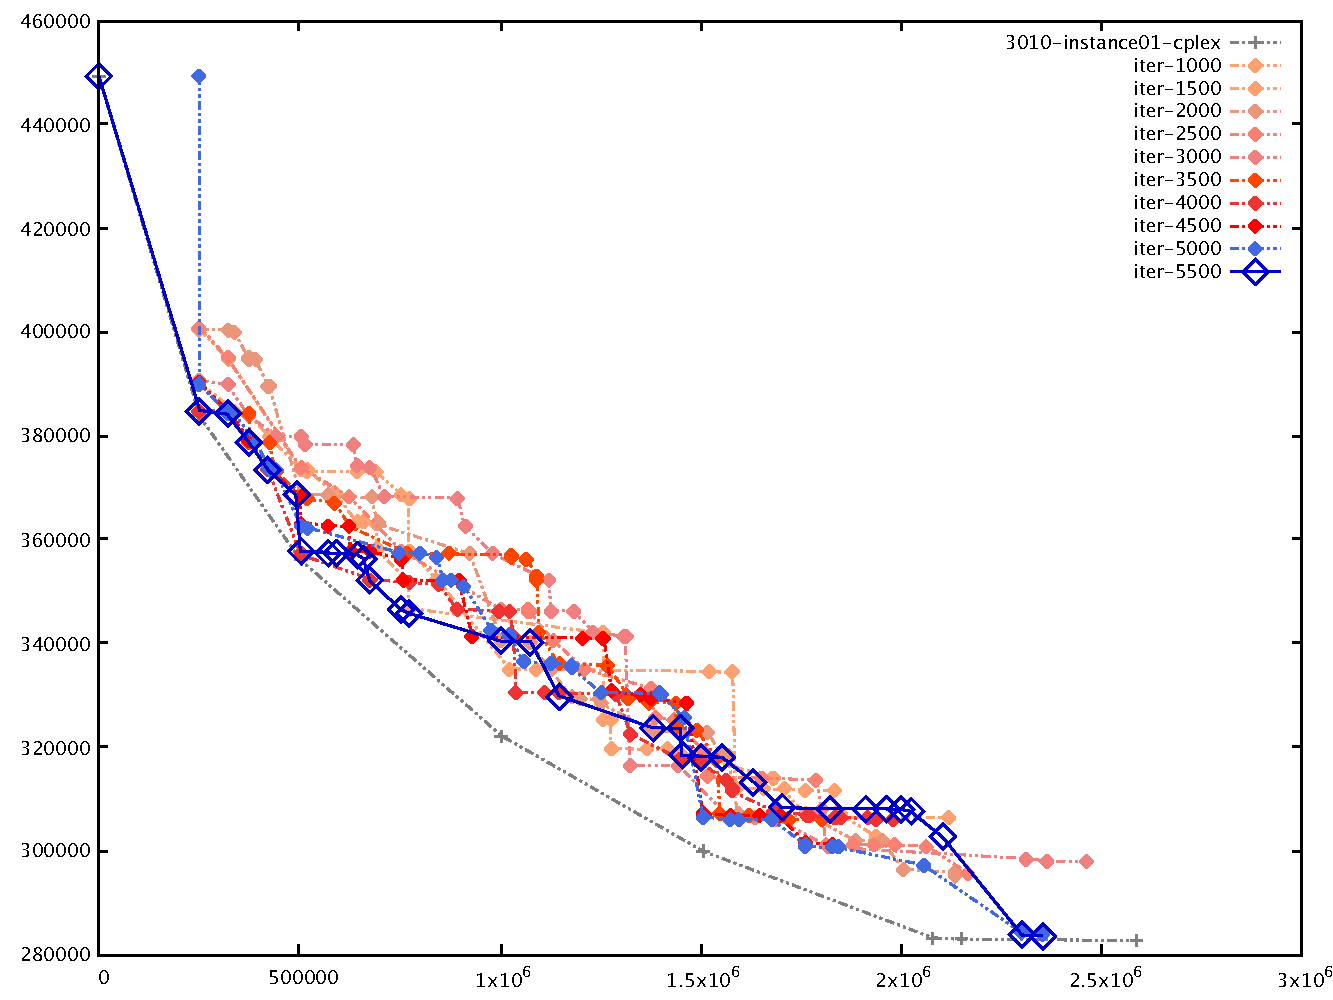
\includegraphics[page=1,width=3.5in]{SMPSO_iterationtest.pdf}}
\caption{SMPSO Iteration Test} 
\label{smpsoitertest}
\end{figure}

\subsection{Particle Swarm Optimized Non-dominated Sorting Genetic Algorithm}\label{psonsga}
As we discussed before, Although NSGAII has better convergence efficiency compared to Particle Swarm Algorithm. NSGAII algorithm suffers from restriction of initial solution set. Without good initial solution, NSGAII has difficulty to reach the whole Pareto front. In contrast, SMPSO algorithm displays better coverage of the whole Pareto front due to the particle relocation mechanism behind PSO. Given enough iteration, SMPSO can always reach extreme point successfully. Which is an important criteria for Pareto front quality. However, PSO algorithm display hardness to push the convergence toward true Pareto front even with extended iterating, as can be seen in \Fig{smpsoitertest}.
The algorithm PSONSGA we proposed here, combines both NSGAII's convergence advantage and SMPSO's coverage advantage. 
For parameter setting of NSGAII and SMPSO subroutine, we use the best parameter setting found in subsection \ref{nsga}, subsection \ref{smpso}.
\begin{table}[H]
\caption{PSONSGA Parameter Selection}
\label{psonsgaparatable}
\centering
\resizebox{\linewidth}{!}{%
\begin{tabular}{ l r r r }
  \toprule
  PSONSGA parameter choice & Experiment group & &Final choice \\
  \midrule
  pso Mutation Distribution Index &  && 18 \\
  pso Mutation Probability & && $ 1 / \textit{number of variable}$\\
  pso Crossover Distribution Index &  && 20\\
  pso Crossover Probability &  && 0.9\\
  pso Swarm Size &  && 1000 \\
  \midrule
  nsga Mutation Distribution Index &  && 20 \\
  nsga Mutation Probability & && $ 1 / \textit{number of variable}$\\
  nsga Crossover Distribution Index &  && 20\\
  nsga Crossover Probability & && 0.9\\
  nsga Population &  && 1000 \\
  \bottomrule
\end{tabular}}
\end{table}
Another question needs to be answered here is how much iteration PSO subroutine needs to explore and how much iteration NSGA needs to push to true front. 
To answer that, we run ten of PSONSGA experiments, using the same parameter setting as Table\ref{psonsgaparatable}, both with 2500 total iterations but different iteration combination for PSO, NSGAII. The results in \Fig{psonsgaitertest} show that, 2250 SMPSO running and 250 NSGAII running is the best. Also, the PSO runs solely ("dark-blue") can achieve good coverage, however, fail to reach good convergence to true front. 
\begin{figure}[H]
\centerline{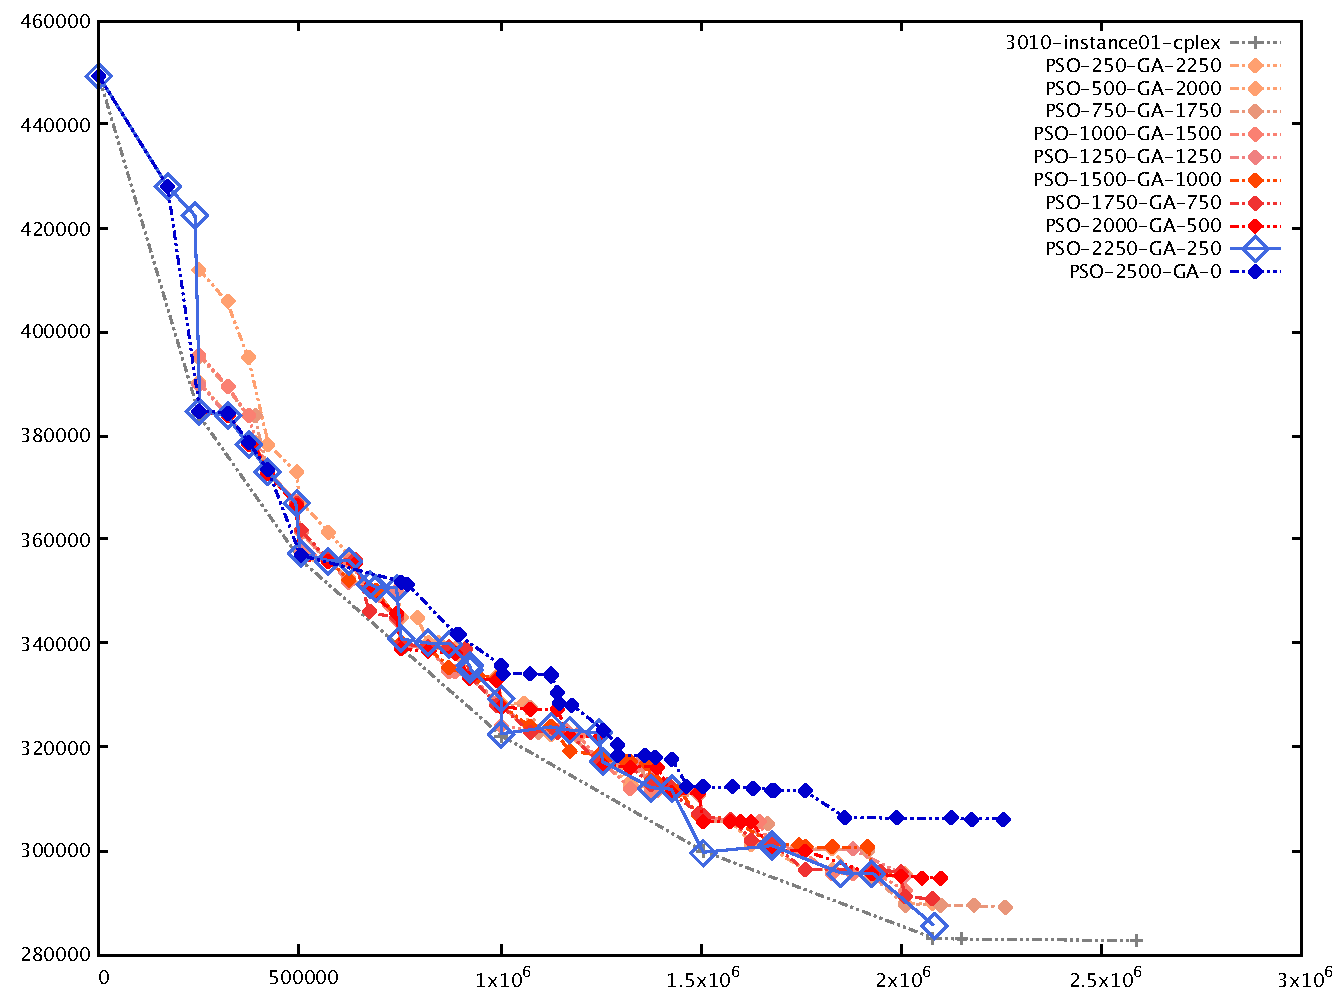
\includegraphics[page=1,width=3.5in]{PSONSGAII_SettingTest.pdf}}
\caption{PSONSGA Iteration Test} 
\label{psonsgaitertest}
\end{figure}

The comparison result of three heuristic algorithm on different size of FPP (30-10, 60-10, 90-10) (Table \ref{table:median.HV}) proves that PSONSGAII performs better in terms of convergence and diversity.
\begin{table}[h]
\caption{Hyper-Volume Indicator on Three Heuristic Algorithms}
\label{table:median.HV}
\resizebox{\linewidth}{!}{%
\begin{tabular}{llll}
\hline & NSGAII & SMPSO &  PSONSGAII\\
\hline
FogPlanningProblem3010 & $  4.95e-01_{ 1.9e-02}$ & \cellcolor{gray25}$  5.52e-01_{ 8.8e-02}$ & \cellcolor{gray95}$  6.15e-01_{ 7.5e-02}$ \\
\hline
FogPlanningProblem6010 & $  2.41e-01_{ 3.6e-02}$ & \cellcolor{gray25}$  3.21e-01_{ 7.3e-02}$ & \cellcolor{gray95}$  3.69e-01_{ 1.4e-01}$ \\
\hline
FogPlanningProblem9010 & $  3.41e-01_{ 2.3e-02}$ & \cellcolor{gray25}$  3.74e-01_{ 5.6e-02}$ & \cellcolor{gray95}$  4.21e-01_{ 2.7e-01}$ \\
\hline
\end{tabular}}
\end{table}

Also, the execution time (Fig \ref{eta}) shows that PSONSGA is highly promising in multi-objective FPP optimization. In particular, when problem size scales up, FPP can be expected to produce near optimal result under reasonable execution time. This property is even prominent if we consider the dynamic extension of current generalized FPP model. 
\begin{figure}[H]
\centerline{\includegraphics[page=1,width=3.5in]{executiontimechart}}
\caption{Execution Time of NSGAII SMPSO PSONSGA and CPLEX} 
\label{eta}
\end{figure}
\fi





% needed in second column of first page if using \IEEEpubid
%\IEEEpubidadjcol


% An example of a floating figure using the graphicx package.
% Note that \label must occur AFTER (or within) \caption.
% For figures, \caption should occur after the \includegraphics.
% Note that IEEEtran v1.7 and later has special internal code that
% is designed to preserve the operation of \label within \caption
% even when the captionsoff option is in effect. However, because
% of issues like this, it may be the safest practice to put all your
% \label just after \caption rather than within \caption{}.
%
% Reminder: the "draftcls" or "draftclsnofoot", not "draft", class
% option should be used if it is desired that the figures are to be
% displayed while in draft mode.
%
%\begin{figure}[!t]
%\centering
%\includegraphics[width=2.5in]{myfigure}
% where an .eps filename suffix will be assumed under latex, 
% and a .pdf suffix will be assumed for pdflatex; or what has been declared
% via \DeclareGraphicsExtensions.
%\caption{Simulation results for the network.}
%\label{fig_sim}
%\end{figure}

% Note that the IEEE typically puts floats only at the top, even when this
% results in a large percentage of a column being occupied by floats.
% However, the Computer Society has been known to put floats at the bottom.


% An example of a double column floating figure using two subfigures.
% (The subfig.sty package must be loaded for this to work.)
% The subfigure \label commands are set within each subfloat command,
% and the \label for the overall figure must come after \caption.
% \hfil is used as a separator to get equal spacing.
% Watch out that the combined width of all the subfigures on a 
% line do not exceed the text width or a line break will occur.
%
%\begin{figure*}[!t]
%\centering
%\subfloat[Case I]{\includegraphics[width=2.5in]{box}%
%\label{fig_first_case}}
%\hfil
%\subfloat[Case II]{\includegraphics[width=2.5in]{box}%
%\label{fig_second_case}}
%\caption{Simulation results for the network.}
%\label{fig_sim}
%\end{figure*}
%
% Note that often IEEE papers with subfigures do not employ subfigure
% captions (using the optional argument to \subfloat[]), but instead will
% reference/describe all of them (a), (b), etc., within the main caption.
% Be aware that for subfig.sty to generate the (a), (b), etc., subfigure
% labels, the optional argument to \subfloat must be present. If a
% subcaption is not desired, just leave its contents blank,
% e.g., \subfloat[].


% An example of a floating table. Note that, for IEEE style tables, the
% \caption command should come BEFORE the table and, given that table
% captions serve much like titles, are usually capitalized except for words
% such as a, an, and, as, at, but, by, for, in, nor, of, on, or, the, to
% and up, which are usually not capitalized unless they are the first or
% last word of the caption. Table text will default to \footnotesize as
% the IEEE normally uses this smaller font for tables.
% The \label must come after \caption as always.
%
%\begin{table}[!t]
%% increase table row spacing, adjust to taste
%\renewcommand{\arraystretch}{1.3}
% if using array.sty, it might be a good idea to tweak the value of
% \extrarowheight as needed to properly center the text within the cells
%\caption{An Example of a Table}
%\label{table_example}
%\centering
%% Some packages, such as MDW tools, offer better commands for making tables
%% than the plain LaTeX2e tabular which is used here.
%\begin{tabular}{|c||c|}
%\hline
%One & Two\\
%\hline
%Three & Four\\
%\hline
%\end{tabular}
%\end{table}


% Note that the IEEE does not put floats in the very first column
% - or typically anywhere on the first page for that matter. Also,
% in-text middle ("here") positioning is typically not used, but it
% is allowed and encouraged for Computer Society conferences (but
% not Computer Society journals). Most IEEE journals/conferences use
% top floats exclusively. 
% Note that, LaTeX2e, unlike IEEE journals/conferences, places
% footnotes above bottom floats. This can be corrected via the
% \fnbelowfloat command of the stfloats package.

\subsection{Result Analysis}\label{resultanalyssi}
In this section, we present the experiment results to assess the performance of the algorithms.
Four instances of 26 different problem sizes are solved by the weighted sum, NSGA-II, SMPSO and PSONSGA algorithms.
A population size of 100 with a number of iterations of 10,000 is used for the three evolutionary algorithms. We use the same parameter settings as the ones described in the last section.
\subsubsection{HV Indicator Comparison}
Since the output of each MO algorithm is a non-dominated solution set, we employ the HV indicator \cite{Auger:2009:THI:1527125.1527138} to evaluate and compare the solution quality between the weighted sum algorithm and the three evolutionary algorithms. 
\iffalse
Table \ref{table:median.HV.nsgaii} shows the HV results for the first instance of the 26 problems. The first column shows the problem number which corresponds to the first column of Table \ref{problemsizes}. The following two columns contain the HV results and the CPU times obtained by solving FPP with the weighted sum method. Column 4 shows the gap (expressed as a percentage) between the solution HV value obtained with the weighted sum, and the best HV value among the four algorithms. The following three columns show the HV value, the corresponding CPU time as well as the gap for the NSGA-II algorithm. The next three columns are the results for the SMPSO algorithm. Finally, similar information for the PSONSGA algorithm is provided in the last three columns. The results for the other three instances are presented in Appendix B1, B2 and B3.

\begin{table}[H]
\caption{HV value and CPU time for instance-1}
\label{table:median.HV.nsgaii}
\centering
\resizebox{0.9\linewidth}{!}{
\footnotesize
\begin{tabular}{|*{13}{c|}}
\hline
\textbf{}&  \multicolumn{3}{c|}{\textbf{Weighted Sum}} & \multicolumn{3}{c|}{\textbf{NSGA-II}}&\multicolumn{3}{c|}{\textbf{SMPSO}}&\multicolumn{3}{c|}{\textbf{PSONSGA}}  \\
\hline
\hline
\textbf{Problem }&\textbf{HV }& \textbf{CPU }& \textbf{Gap} 
&\textbf{HV }& \textbf{CPU }& \textbf{Gap }
&\textbf{HV }& \textbf{CPU }& \textbf{Gap }
&\textbf{HV }& \textbf{CPU }& \textbf{Gap} \\
   \textbf{\#}&&\textbf{(s)}&\textbf{\%}
      &&\textbf{(s)}&\textbf{\%}   
      &&\textbf{(s)}&\textbf{\%}
         &&\textbf{(s)}&\textbf{\%}\\
   \hline
1&0.488&1&14.26&0.558&3&0.00&0.558&1&0.00&0.558&1&0.00\\
2&0.461&1&27.25&0.582&3&0.69&0.575&1&1.91&0.586&2&0.00\\
3&0.545&1&15.86&0.632&3&0.00&0.623&1&1.44&0.610&2&3.61\\
4&0.506&7&20.52&0.567&3&7.58&0.591&1&3.21&0.610&2&0.00\\
5&0.519&8&19.76&0.531&3&17.14&0.614&1&1.30&0.622&2&0.00\\
6&0.427&10&36.14&0.545&3&6.61&0.554&2&4.87&0.581&4&0.00\\
7&0.508&9&20.20&0.522&3&17.05&0.578&2&5.71&0.611&4&0.00\\
8&0.498&46&20.32&0.486&4&23.25&0.566&2&5.83&0.599&5&0.00\\
9&0.526&45&21.77&0.507&5&26.23&0.640&2&0.00&0.613&7&4.40\\
10&0.404&41&36.21&0.338&5&62.72&0.510&3&7.84&0.550&7&0.00\\
11&0.483&50&20.83&0.438&10&33.11&0.549&3&6.19&0.583&12&0.00\\
12&0.506&62&18.55&0.459&18&30.72&0.548&6&9.49&0.600&16&0.00\\
13&0.552&698&20.23&0.544&184&22.06&0.639&286&3.91&0.664&251&0.00\\
14&0.509&854&25.06&0.451&1747&41.02&0.598&301&6.35&0.636&343&0.00\\
15&0.548&2777&23.25&0.506&1729&33.60&0.676&315&0.00&0.653&339&3.52\\
16&0.484&7390&29.89&0.425&1757&48.00&0.592&320&6.25&0.629&1324&0.00\\
17&0.523&4478&22.72&0.467&1891&37.47&0.601&333&6.82&0.642&2538&0.00\\
18&0.548&8204&16.00&0.432&2055&47.22&0.595&341&6.89&0.636&2724&0.00\\
19&0.461&9392&28.27&0.340&2145&73.82&0.551&554&7.26&0.591&2833&0.00\\
20&0.547&20921&17.95&0.411&2175&56.93&0.611&659&5.56&0.645&4858&0.00\\
21&0.476&22022&27.36&0.362&2078&67.40&0.533&954&13.70&0.606&4962&0.00\\
22&0.470&11147&27.35&0.300&2126&99.67&0.561&1236&6.77&0.599&3805&0.00\\
23&0.321&19403&74.07&0.327&2952&70.95&0.559&1444&0.00&0.535&4424&4.49\\
24&0.356&19476&61.55&0.271&3621&112.18&0.515&1314&11.65&0.575&4172&0.00\\
25&0.487&25422&18.29&0.295&3323&95.25&0.542&1489&6.27&0.576&4847&0.00\\
26&0.452&19510&27.86&0.249&5353&132.13&0.518&1639&11.58&0.578&5464&0.00\\

\hline

\hline
\end{tabular}}
\end{table}
\fi
HV indicator examines both the convergence and diversity properties of a solution set. In these perspectives, PSONSGA algorithm displays its superiority in finding a good quality solution within reasonable computation time. In fact, for all four problem instances (a total of 104 different problems), PSONSGA provides the best HV value for 95 problems (91.3\%). The NSGA-II and SMPSO each provides the highest HV value for 19 different problems (18.2\%). The weighted sum approach only provides the best HV value for 2 problems (1.92\%).

\Fig{hvaverage} provides a complete comparison of the HV values amongst the weighted sum, NSGA-II, SMPSO and PSONSGA algorithms over the four instance sets with a 95\% confidence interval.
\begin{figure}[h]
\centerline{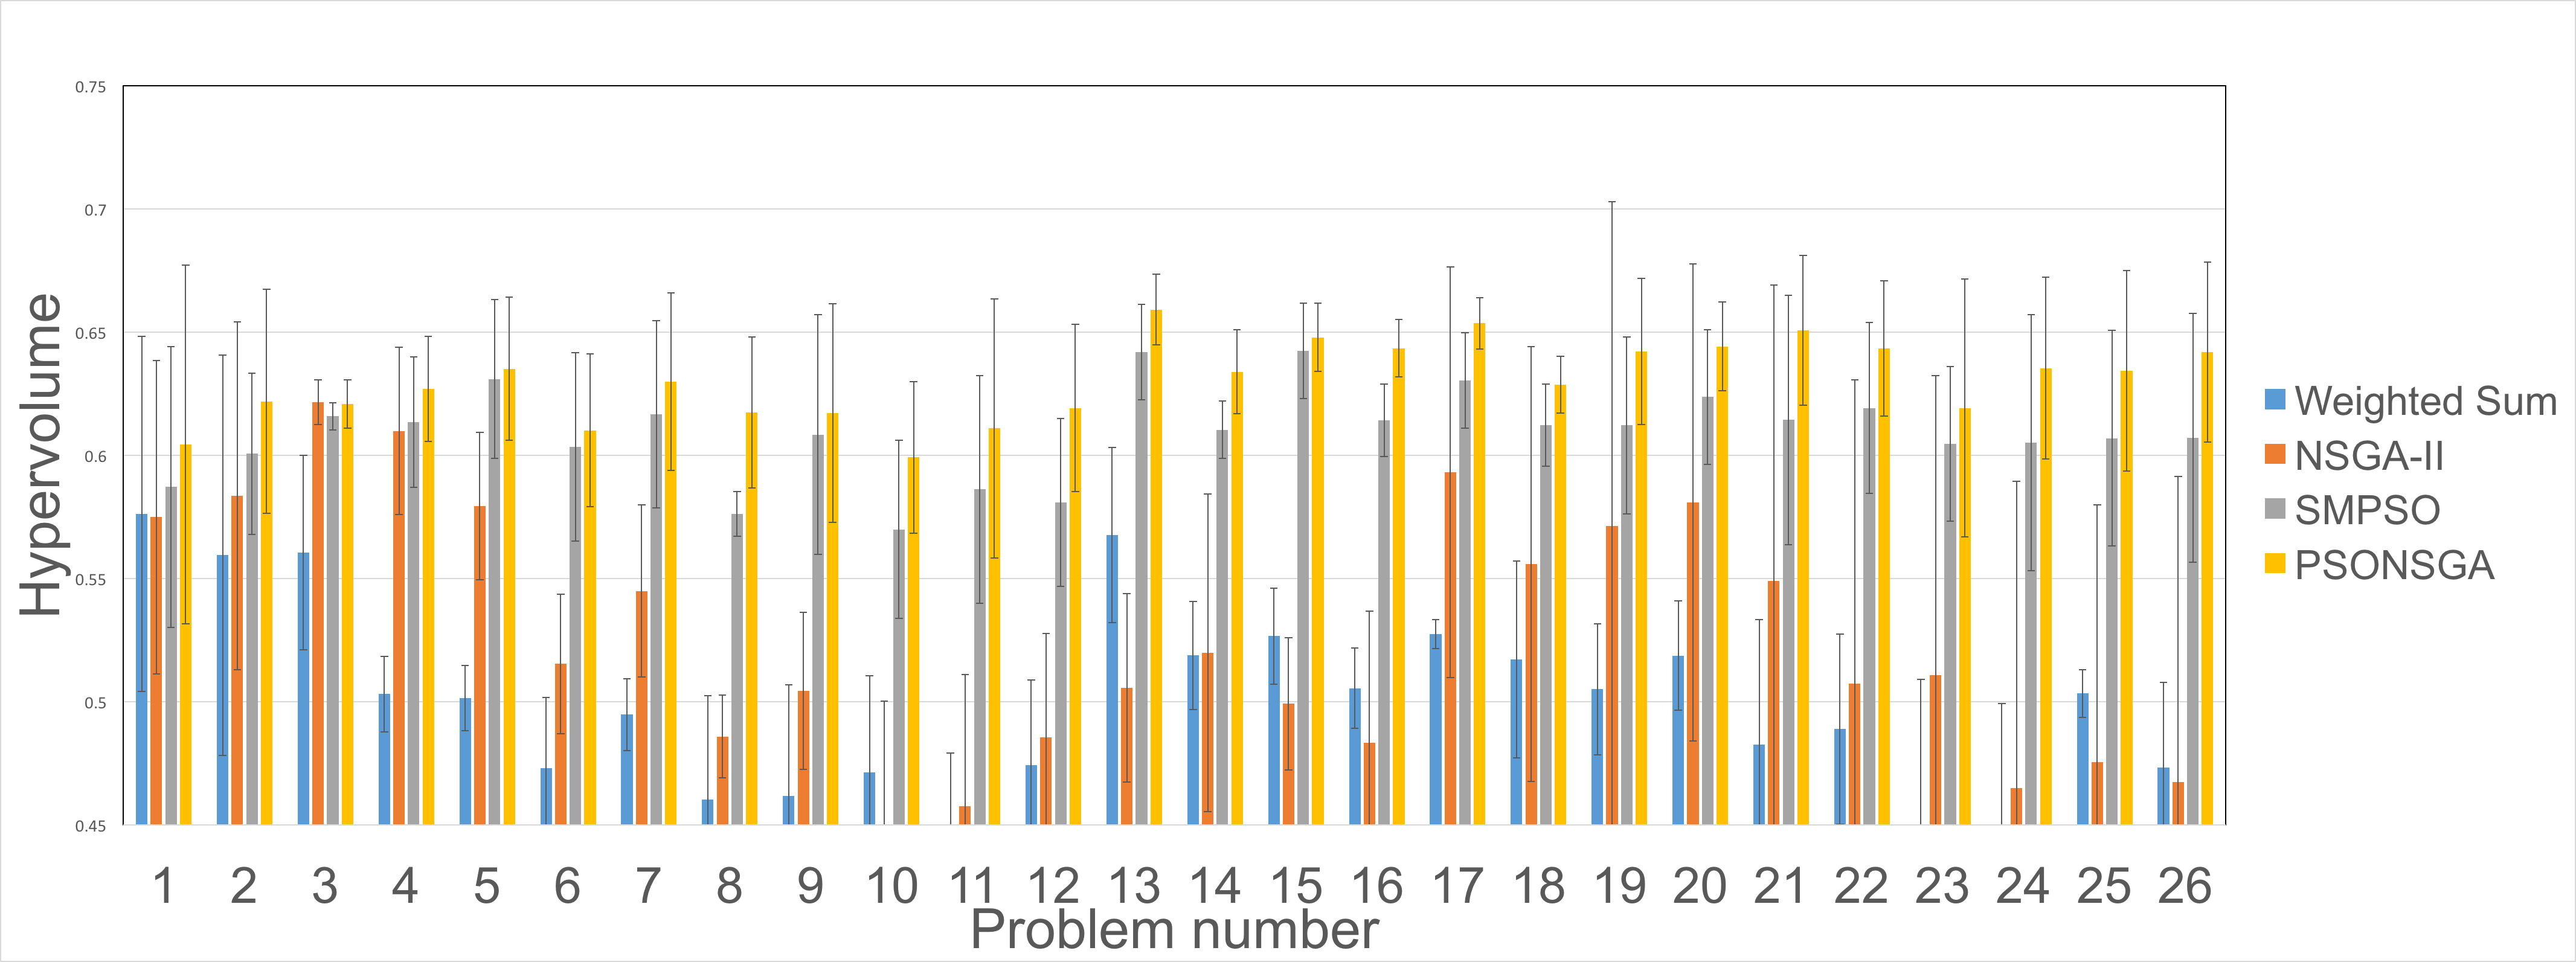
\includegraphics[page=1,width=3.5in]{hvaverageoverfour.png}}
\caption{HV indicator comparison (over four instance sets)} 
\label{hvaverage}
\end{figure}
As shown in \Fig{hvaverage}, the PSONSGA algorithm achieves the best balance between convergence and diversity amongst the three evolutionary algorithms. The weighted sum approach produces worse HV values, because each individual branch and bound search can only produce one single solution. We can also notice that for large-scale problems, NSGA-II's HV values are worse than all three other algorithms. This is due to the larger search space in large-scale problems and the concentrated effect of the non-dominated sorting in the NSGA-II algorithm.
\subsubsection{IGD Indicator Comparison}

\iffalse
\Fig{} further presents a  HV comparison  As shown in \Fig{hvaverage}, we can reach the same conclusion that PSONSGA outperforms the weighted sum method and the two existing EMO algorithms in HV tests.
\fi


In this section, we examine the solution quality of the weighted sum, NSGA-II, SMPSO and PSONSGA algorithms by using the IGD quality indicator. As discussed in Chapter 2, the IGD indicator evaluates the quality of a solution set using a reference set. It generates the IGD value through calculating the average euclidean distance between the solution sets and the reference sets. In our evaluation, we use the best non-dominated solutions returned by all three methods as the reference set. The IGD values for the four algorithms are presented in Table \ref{table:igd}. The first column shows the problem number. Columns 2, 3, 4 and 5 display respectively, the average IGD value for the weighted sum, NSGA-II, SMPSO and PSONSGA. 
As shown in Table \ref{table:igd}, PSONSGA displays its superiority over the weighted sum method and the two existing evolutionary algorithms in this evaluation. The average IGD values for PSONSGA's solution achieves the best IGD in 25 of the 26 problems. This improvement over NSGA-II and SMPSO can be explained by the information exchange between the PSO and GA phases in the PSONSGA procedure. %The result from the PSO provides the GA a good search basis. Then, the genetic search keeps track of this information to do an intensive search through non-dominated sorting and aggressive selection.
This two-phase procedure has been proven to reach better Pareto front results as shown by the IGD indicator comparison.


\begin{table}[h]
\caption{IGD indicator comparison (average over four instances)}\label{table:igd}
\centering
\begin{scriptsize}
\resizebox{\columnwidth}{!}{
\begin{tabular}{|*{5}{c|}}
\hline \textbf{Problem \#}&\textbf{Weighted sum}& \textbf{NSGA-II }& \textbf{SMPSO} &  \textbf{PSONSGA}\\
\hline
\hline
1 &$2.16E-01$&$1.01E-02$&$2.01E-03 $&\cellcolor{gray95}$1.43E-03$\\
2 &$1.31E-01$&$9.22E-03$&$2.09E-03 $&\cellcolor{gray95}$1.24E-03$\\
3 &$9.81E-02$&$4.95E-03$&$1.96E-03 $&\cellcolor{gray95}$1.11E-03$\\
4 &$4.11E-02$&$1.24E-02$&$2.46E-03 $&\cellcolor{gray95}$1.97E-03$\\
5 &$3.57E-02$&$1.30E-02$&$3.16E-03 $&\cellcolor{gray95}$3.02E-03$\\
6 &$3.57E-02$&$1.32E-02$&$3.55E-03 $&\cellcolor{gray95}$2.49E-03$\\
7 &$6.12E-02$&$1.17E-02$&$3.73E-03 $&\cellcolor{gray95}$2.81E-03$\\
8 &$9.72E-02$&$1.99E-02$&$3.68E-03 $&\cellcolor{gray95}$2.44E-03$\\
9 &$9.83E-02$&$1.79E-02$&$4.44E-03 $&\cellcolor{gray95}$3.28E-03$\\
10&$1.13E-01$&$1.73E-02$&$5.32E-03$&\cellcolor{gray95}$3.83E-03$\\
11&$1.34E-01$&$2.06E-02$&$4.98E-03$&\cellcolor{gray95}$3.52E-03$\\
12&$1.40E-01$&$2.08E-02$&$5.54E-03$&\cellcolor{gray95}$4.33E-03$\\
13&$4.47E-02$&$1.57E-02$&$2.37E-03$&\cellcolor{gray95}$1.48E-03$\\
14&$5.21E-02$&$1.78E-02$&$2.59E-03$&\cellcolor{gray95}$1.69E-03$\\
15&$7.05E-02$&$1.68E-02$&$2.40E-03$&\cellcolor{gray95}$1.69E-03$\\
16&$1.24E-01$&$1.70E-02$&$3.11E-03$&\cellcolor{gray95}$2.05E-03$\\
17&$1.18E-01$&$1.51E-02$&$3.53E-03$&\cellcolor{gray95}$2.53E-03$\\
18&$1.82E-01$&$1.70E-02$&$3.50E-03$&\cellcolor{gray95}$2.33E-03$\\
19&$1.70E-01$&$1.52E-02$&$3.32E-03$&\cellcolor{gray95}$2.59E-03$\\
20&$3.03E-01$&$1.76E-02$&$3.43E-03$&\cellcolor{gray95}$2.25E-03$\\
21&$2.62E-01$&$1.64E-02$&$3.86E-03$&\cellcolor{gray95}$3.00E-03$\\
22&$3.03E-01$&$1.92E-02$&$3.61E-03$&\cellcolor{gray95}$2.03E-03$\\
23&$3.48E-01$&$1.53E-02$&$3.66E-03$&\cellcolor{gray95}$2.78E-03$\\
24&$4.03E-01$&$1.97E-02$&$3.34E-03$&\cellcolor{gray95}$2.17E-03$\\
25&$3.68E-01$&$1.65E-02$&\cellcolor{gray95}$3.66E-03$&$3.97E-03$\\
26&$5.32E-01$&$1.93E-02$&$4.43E-03$&\cellcolor{gray95}$4.27E-03$\\\hline
\end{tabular}}
\end{scriptsize}
\end{table}



\subsubsection{Delay Gap Comparison}
Since we solved the weighted sum formulation with CPLEX solver, each solution point from the CPLEX solver is an optimal solution. In other words, under the same expense condition, the traffic delay produced by the weighted sum and CPLEX can achieve the optimum. Using CPLEX solutions as the reference, we calculate the average delay gaps between CPLEX and the evolutionary algorithms. The average delay gaps were computed only if the same cost exists in the weighted sum solution sets and CPLEX has found the optimal solutions (the relative MIP equals to zero). 
\iffalse
\Fig{delaygapinstanc1} presents the comparison in terms of delay gaps between the three evolutionary algorithms for problems of first instance. As shown in \Fig{delaygapinstanc1},  NSGA-II comes in the first place in terms of the delay gaps over 26 problems with an average gap of 0.3\% . PSONSGA gives the second best performance with less than or equal to the delay in NSGA-II in 12 of 26 problems with an average gap of 0.4\%. An intensive statistical analysis for delay gaps is presented in Table \ref{delaygapss}
\begin{figure}[H]
\centerline{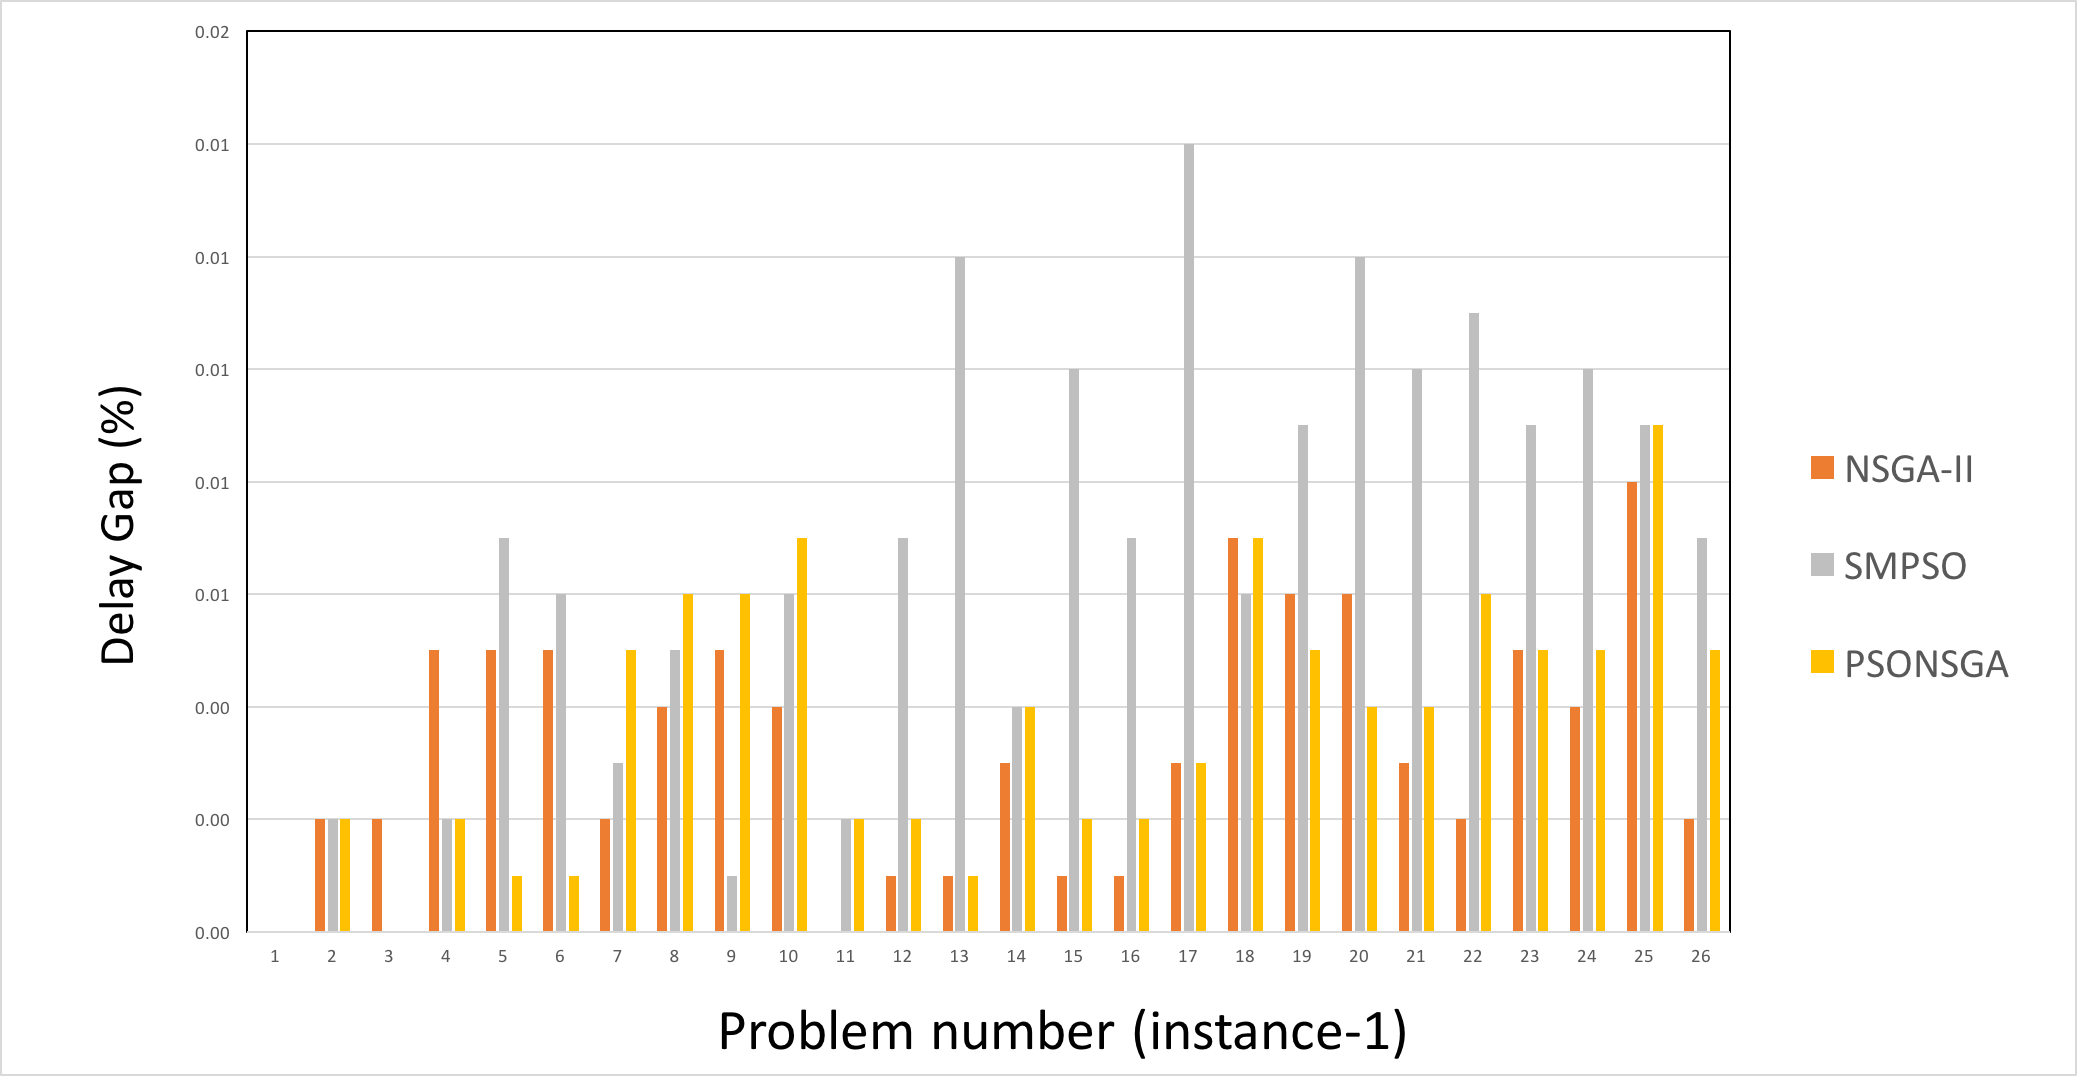
\includegraphics[page=1,width=5.5in]{delaygapfiture.png}}
\caption{Delay gaps (instance-1)} 
\label{delaygapinstanc1}
\end{figure}
\fi
Table \ref{delaygapss} shows the statistical analysis for delay gaps over the four instance sets. The first three columns represent the minimum, the maximum, and the average delay gaps. The following two columns are the standard deviation and the 95\% confidence interval for the average delay gaps. As shown in Table \ref{delaygapss}, without considering the diversity and distribution in solution sets, NSGA-II gives the best delay gaps to optimal solutions. The reason behind this is the non-dominated sorting in NSGA-II concentrates the solution sets towards the optimal front. However, this sorting process sacrifices the solution diversity for a better convergence quality. This is the same reason why the solutions produced by the NSGA-II algorithm provide worse HV values. PSONSGA achieves the second best among the three evolutionary algorithms.
\begin{table}[h]
\centering
\caption{Delay gap comparison (over four instance sets)}\label{delaygapss}
\resizebox{\columnwidth}{!}{
\begin{tabular}{|*{7}{c|}}
\hline
\textbf{Algorithms}& \textbf{Min.gap} & \textbf{Max.gap }&\textbf{Ave.gap} &\textbf{Std.dev}&\textbf{95\% C.I.}\\
&\textbf{(\%)} &\textbf{(\%)}&\textbf{(\%)}&\textbf{(\%)}&\textbf{(\%)}\\
\hline
 NSGA-II&0.00&7.80&0.30&0.81&0.30$\pm$0.15\\
SMPSO&0.00&8.50&0.60&1.19&0.60$\pm$0.22\\
PSONSGA&0.00&7.80&0.50&1.12&0.50$\pm$0.21\\
\hline
\end{tabular}}
\end{table}
\subsubsection{CPU Time Comparison}
\Fig{cputimeover4} provides the comparison in terms of the CPU time between the weighted sum method and the three evolutionary algorithms over the four instance sets with a 95\% confidence interval. 
\iffalse
\begin{figure}[H]
\centerline{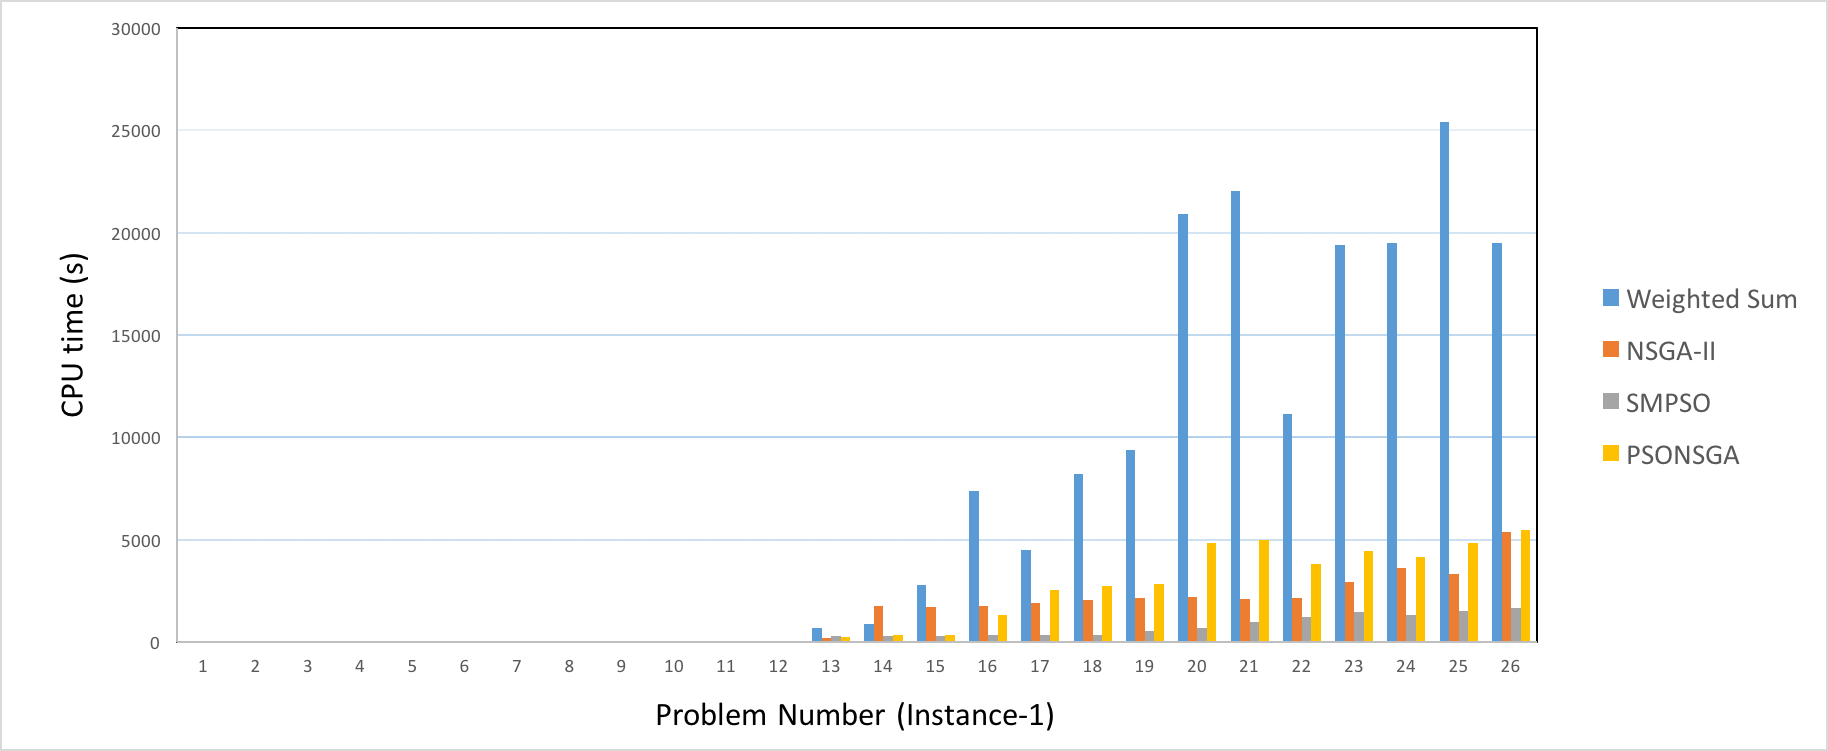
\includegraphics[page=1,width=5.5in]{nv26cputime.png}}
\caption{CPU time comparison (instance-1)} 
\label{cputimecomparison}
\end{figure}
\fi
As shown in \Fig{cputimeover4}, all three evolutionary algorithms can provide good quality Pareto frontier in a reasonable amount of time. For small-scale problems (problems 1 to 12), the three evolutionary algorithms can finish the optimization within 30 seconds. For large-scale problems, evolutionary algorithms' solution times are still within a reasonable range. For example, to solve problem 26 (instance-1), NSGA-II, SMPSO, PSONSGA, each respectively took 5,303 seconds, 1,639 seconds and 5,464 seconds. In comparison, the weighted sum method using the Cplex solver takes 19,510 seconds, which is approximately 3.5 times longer than PSONSGA. We also notice that, although fast for small size problems, CPLEX's CPU time is almost increasing exponentially with respect to the problem size. This corresponds with the fact that the fog planning problem is NP-hard as described before.
\iffalse
\Fig{cputimeover4} further presents a complete CPU time comparison  As shown in \Fig{cputimeover4}, we can reach the same conclusion that all three evolutionary algorithms can generate close-to-optimal solutions in a reasonable amount of time.
\fi
\begin{figure}[h]
\centerline{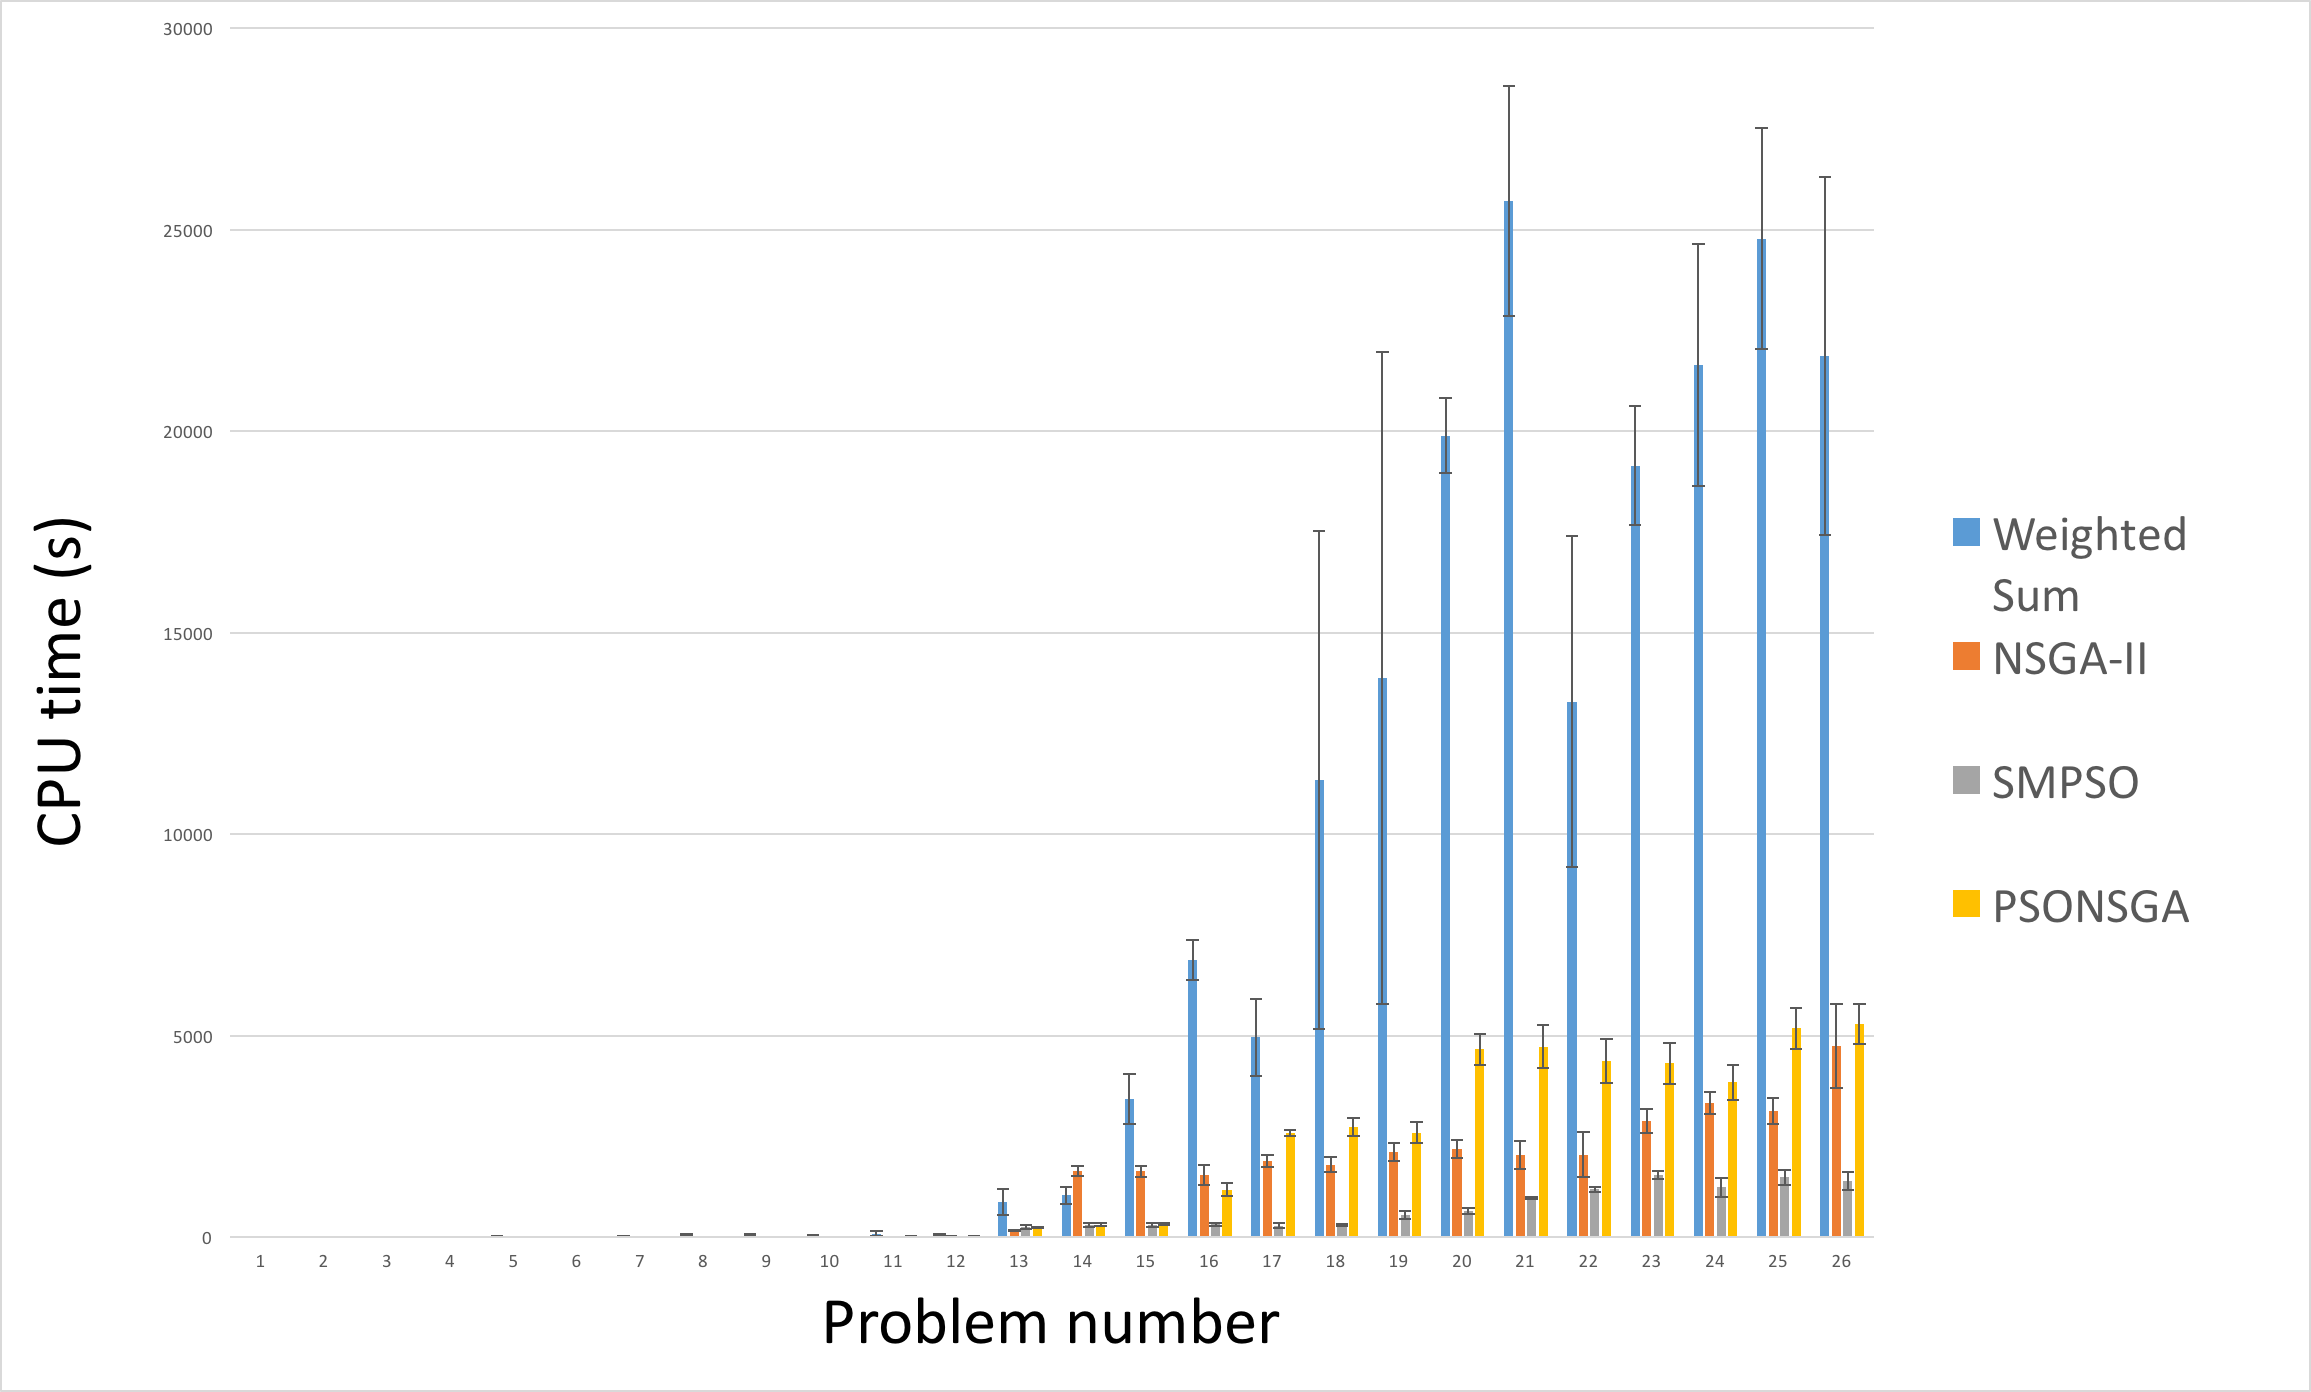
\includegraphics[page=1,width=3.5in]{cputimeover4}}
\caption{CPU time comparison (over four instance sets)} 
\label{cputimeover4}
\end{figure}


From the delay gap comparison shown in Table \ref{delaygapss} and the CPU time comparison in \Fig{cputimeover4}, we can conclude that the evolutionary algorithms are able to use less CPU time to generate close to optimal solutions. At the same time, PSONSGA attains a good balances between the solution convergence and diversity, compared to the two existing algorithms (NSGA-II and SMPSO).









\section{Related Works}\label{relwork}
Fog computing research has attracted lots of attention. Researchers have been working on studies of fog architecture \cite{fcsmartcity}, fog communication protocols \cite{Peng:2016:FRA:3029494.3029575} and application logic in fog networks \cite{SUN2017687}. Regarding workload allocation and resource management in fog computing networks, Dsouza et al.\cite{secme} proposed a policy-based resource management in fog computing, which expanded the current fog computing platform to support collaboration and interoperability between different resources. Deng et al., in \cite{fcworkload}, focused on investigating the tradeoff between power consumption and transmission delay in the fog-cloud computing system, and they formulated a work-load allocation problem that aims at minimal power consumption considering the constrained service delay. Sun and Zhang \cite{SUN2017687} proposed a fog computing structure to integrate spare resources in the network applying a crowd-funding algorithm.
Among all the work describe above that are directly focusing on the fog computing environment, none of them addresses the planning and design of fog networks as we are presenting it in this paper. 

Another closely related topic under the network planning context is the distributed-cloud planning. 
Hwang et al \cite{hwang2013distributed} illustrated the planning processes of creating high-performance, scalable, reliable distributed computing systems including the design principles, architectures, and innovative applications. 
Khosravi and Buyya \cite{enerfoot} presented a taxonomy and classification of the existing techniques for resource management in achieving a green cloud computing environment. 
Iturriaga et al. \cite{ITOR:ITOR12294} studied the application of multi-objective evolutionary algorithms for solving the energy-aware scheduling problem. The scheduling problem took account of the scheduling of large workflows in a federation of datacenters. In another study, Xu and Li, in \cite{6566873}, presented a joint request mapping and response routing policy for geo-distributed cloud services. The utility functions were used to capture the performance goals. However, their model focused on the resource mapping and traffic routing in distributed cloud networks without considering the placement and sizing of the geo-distributed cloud. 
Among all the work describe above that are directly related to the distributed-cloud planning, none of them addresses the facility planning and provisioning in distributed computing networks as we are presenting it in this paper.



\section{Conclusion}\label{conclu}
We proposed a multi-objective modular facility location model for planning Fog Network. The multi-objective combinatorial model enables us to fully explore the searching domain with different fog location selection, fog type selection and user allocation combinations. The model produces the Pareto front solution set over two objectives: the network delay and the building cost. Decision maker can use this Pareto front to make reliable decision on fog infrastructure building plan. 
And we propose to apply exact algorithm (weighted sum) and heuristic algorithm (NSGAII, SMPSO and PSONSGA) to solve the model. The results from the weighted sum, NSGA-II, SMPSO and PSONSGA are compared in terms of the HV indicator, IGD indicator and delay gaps. The experimental results confirm that evolutionary algorithms can be notably efficient in execution time compared to the weighted sum based approach. From the HV and IGD indicator perspectives, PSONSGA achieves the best HV and IGD values for most of the problem sizes. In contrast, NSGA-II was able to return good solutions in terms of the delay objective value without considering the diversity and coverage of solution frontiers.
In the real world of fog planning, the number of edge-clusters can be extremely large, and the network topology, conditions and restrictions will be more complicated. Therefore, using the weighed sum method and CPLEX can be time-consuming. In fact, the proposed algorithm can be more appropriate in this situation. PSONSGA is recommended for solving the fog planning problem as it achieves the best balance between the solution diversity, convergence and computation time.


% It means that to evaluate the performance of exact and approximation algorithms, 26 different problem sizes were solved. 
%The PSONSGA algorithm proposed in this paper improve the \\

%In this chapter, we applied weighted sum and three multi-objective heuristic algorithms to the FPP problems. The results of these experiments and comparisons in \Sec{resultanalyssi}, demonstrated that our optimization approaches, including the evolutionary algorithm we proposed in this work are capable of finding excellent Pareto frontier solutions within reasonable computation time. All these high-quality Pareto frontiers allow the decision maker to balance and evaluate for more informed FPP decision making.



In future, our model can be further extended to dynamic expansion model, in which existing fog facility can be partially closed and reopened later at any time period. The fog site can be relocated to accommodate seasonal traffic changes. The same heuristic algorithm such as PSONSGA can be apply on this extension. Considering its highly solution time efficiency, PSONSGA can be even promising on this problem, especially, because the dynamic model problem with time periods could easily scale up. In this context, exact algorithm such as Weighted Sum can be struggling to produce result.





% if have a single appendix:
%\appendix[Proof of the Zonklar Equations]
% or
%\appendix  % for no appendix heading
% do not use \section anymore after \appendix, only \section*
% is possibly needed

% use appendices with more than one appendix
% then use \section to start each appendix
% you must declare a \section before using any
% \subsection or using \label (\appendices by itself
% starts a section numbered zero.)
%

\iffalse
\appendices
\section{Proof of the First Zonklar Equation}
Appendix one text goes here.

% you can choose not to have a title for an appendix
% if you want by leaving the argument blank
\section{}
Appendix two text goes here.


% use section* for acknowledgment
\ifCLASSOPTIONcompsoc
  % The Computer Society usually uses the plural form
  \section*{Acknowledgments}
\else
  % regular IEEE prefers the singular form
  \section*{Acknowledgment}
\fi


The authors would like to thank...
\fi

% Can use something like this to put references on a page
% by themselves when using endfloat and the captionsoff option.
\ifCLASSOPTIONcaptionsoff
  \newpage
\fi



% trigger a \newpage just before the given reference
% number - used to balance the columns on the last page
% adjust value as needed - may need to be readjusted if
% the document is modified later
%\IEEEtriggeratref{8}
% The "triggered" command can be changed if desired:
%\IEEEtriggercmd{\enlargethispage{-5in}}

% references section

% can use a bibliography generated by BibTeX as a .bbl file
% BibTeX documentation can be easily obtained at:
% http://mirror.ctan.org/biblio/bibtex/contrib/doc/
% The IEEEtran BibTeX style support page is at:
% http://www.michaelshell.org/tex/ieeetran/bibtex/
\bibliographystyle{IEEEtran}
% argument is your BibTeX string definitions and bibliography database(s)
\bibliography{IEEEabrv,decheng}
%
% <OR> manually copy in the resultant .bbl file
% set second argument of \begin to the number of references
% (used to reserve space for the reference number labels box)
%\begin{thebibliography}{1}

%\bibitem{IEEEhowto:kopka}
%H.~Kopka and P.~W. Daly, \emph{A Guide to \LaTeX}, 3rd~ed.\hskip 1em plus
 % 0.5em minus 0.4em\relax Harlow, England: Addison-Wesley, 1999.

%\end{thebibliography}

% biography section
% 
% If you have an EPS/PDF photo (graphicx package needed) extra braces are
% needed around the contents of the optional argument to biography to prevent
% the LaTeX parser from getting confused when it sees the complicated
% \includegraphics command within an optional argument. (You could create
% your own custom macro containing the \includegraphics command to make things
% simpler here.)
%\begin{IEEEbiography}[{\includegraphics[width=1in,height=1.25in,clip,keepaspectratio]{mshell}}]{Michael Shell}
% or if you just want to reserve a space for a photo:

\begin{IEEEbiography}{Michael Shell}
Biography text here.
\end{IEEEbiography}

% if you will not have a photo at all:
\begin{IEEEbiographynophoto}{John Doe}
Biography text here.
\end{IEEEbiographynophoto}

% insert where needed to balance the two columns on the last page with
% biographies
%\newpage

\begin{IEEEbiographynophoto}{Jane Doe}
Biography text here.
\end{IEEEbiographynophoto}

% You can push biographies down or up by placing
% a \vfill before or after them. The appropriate
% use of \vfill depends on what kind of text is
% on the last page and whether or not the columns
% are being equalized.

%\vfill

% Can be used to pull up biographies so that the bottom of the last one
% is flush with the other column.
%\enlargethispage{-5in}



% that's all folks
\end{document}


